%                                     MMMMMMMMM        
%                                                                             
%  MMO    MM   MMMMMM  MMMMMMM   MM    MMMMMMMM   MMD   MM  MMMMMMM MMMMMMM   
%  MMM   MMM   MM        MM     ?MMM              MMM$  MM  MM         MM     
%  MMMM 7MMM   MM        MM     MM8M    MMMMMMM   MMMMD MM  MM         MM     
%  MM MMMMMM   MMMMMM    MM    MM  MM             MM MMDMM  MMMMMM     MM     
%  MM  MM MM   MM        MM    MMMMMM             MM  MMMM  MM         MM     
%  MM     MM   MMMMMM    MM   MM    MM            MM   MMM  MMMMMMM    MM
%
%
%            - META-NET Language White Paper | French content -
% 
% ----------------------------------------------------------------------------

\begin{document}

\maketitle

% --------------------------------------------------------------------------
\bsection*{Préface --- Preface}

\null
\pagestyle{empty} 

\pagenumbering{Roman} 
\setcounter{page}{3}
\pagestyle{scrheadings}

\begin{Parallel}[c]{78mm}{78mm}
\ParallelLText{\selectlanguage{french} 
Ce livre blanc fait partie d'une collection qui a pour
objectif de faire connaître le potentiel des technologies de la
langue. Il s'adresse en particulier aux journalistes,
politiciens, communautés linguistiques, enseignants mais aussi à
tous. La disponibilité et l'utilisation des technologies de la
langue variant grandement d'une langue à l'autre en
Europe, les actions nécessaires au soutien des activités de recherche
et développement peuvent être très différentes en fonction des langues
selon des facteurs multiples, comme leur complexité intrinsèque ou
leur nombre de locuteurs.

Le Réseau d'Excellence META-NET, financé par la Commission
Européenne, a analysé l'état des ressources et des
technologies de la langue dans cette collection de livres blancs
(p.~\pageref{whitepaperseries}). Cette étude, qui a concerné les 23
langues officielles de l’Union Européenne ainsi que des langues
nationales et régionales de l’Europe, montre qu’il y a des déficits
énormes en termes de soutien technologique et des lacunes
significatives en recherche selon les langues. L’analyse de la
situation actuelle permettra de maximiser l’impact des futures
recherches.

En mars 2012, META-NET regroupe 54 centres de recherche de 33 pays
européens (p.~\pageref{metanetmembers}) et travaille avec les acteurs
de l’économie (sociétés informatiques, fournisseurs de technologies,
utilisateurs), les agences gouvernementales et non gouvernementales,
les organismes de recherche, les communautés linguistiques et les
universités européennes, pour établir une vision commune des
technologies de la langue et un échéancier stratégique de recherche
dans la vision de l’Europe multilingue de 2020.}

\ParallelRText{\selectlanguage{english}
This white paper is part of a series that promotes knowledge about
language technology and its potential. It addresses journalists,
politicians, language communities, educators and others.  The
availability and use of language technology in Europe varies between
languages. Consequently, the actions that are required to further
support research and development of language technologies also
differs. The required actions depend on many factors, such as the
complexity of a given language and the size of its community.

META-NET, a Network of Excellence funded by the European Commission,
has conducted an analysis of current language resources and
technologies in this white paper series
(p.~\pageref{whitepaperseries}). The analysis focused on the 23
official European languages as well as other important national and
regional languages in Europe. The results of this analysis suggest
that there are tremendous deficits in technology support and
significant research gaps for each language. The given detailed expert
analysis and assessment of the current situation will help maximise
the impact of additional research.

As of March 2012, META-NET consists of 54 research centres from 33
European countries (p.~\pageref{metanetmembers}). META-NET is working
with stakeholders from economy (Software companies, technology
providers, users), government agencies, research organizations,
non-governmental organizations, language communities and European
universities. Together with these communities, META-NET is creating a
common technology vision and strategic research agenda for
multilingual Europe 2020.}  \ParallelPar
\end{Parallel}

\makefundingnotice


% --------------------------------------------------------------------------

\cleardoublepage

\bsection*{Table des matières --- Table of Contents}

\renewcommand\contentsname{}

\tableofcontents

\addtocontents{toc}{\protect\thispagestyle{empty}\protect}
\addtocontents{toc}{{\Large\textsf{\centerline{LA LANGUE FRANÇAISE À L'ÈRE DU NUMÉRIQUE}}\par}}

% --------------------------------------------------------------------------

\cleardoublepage

\setcounter{page}{1}
\pagenumbering{arabic} 
\pagestyle{scrheadings}

\selectlanguage{french}

\begin{french}

\ssection[Résumé exécutif]{Résumé exécutif}

\begin{multicols}{2}

Le multilinguisme est une donnée essentielle de la construction Européenne. Il est primordial d’assurer à chaque citoyen européen la possibilité d’utiliser sa langue maternelle et à chaque Etat européen la capacité de préserver sa culture, tout comme il est essentiel de permettre la communication entre les citoyens pour franchir la barrière des langues dans l’espace informationnel ou commercial communautaire. Ce même besoin existe de fait à l’échelle de la planète.

Peut-on accepter de voir disparaître des langues européennes, et les cultures dont elles font partie~? Du seul fait de la barrière des langues, peut-on accepter de se borner à constater la faiblesse de la croissance du marché européen~? De ne pas avoir accès à la richesse culturelle des autres pays~? De ne pas connaître à leur source les informations qui forgent l’Europe~?

Le multilinguisme a un coût, important, qui fait que progressivement les langues disparaissent au profit des langues majoritaires. Sur les quelques 6500 langues qui existent sur la planète, il est estimé que la moitié auront disparu à la fin de ce siècle. De nombreuses langues européennes ont déjà disparu, ou ont failli disparaître et n’ont été sauvées que grâce à une volonté politique.

Comment traiter les 48 heures de vidéos qui arrivent toutes les minutes sur YouTube, dans toutes les langues~? Comment faire en sorte que les brevets européens soient accessibles pour les entreprises européennes autres que celles qui parlent anglais, français ou allemand~? Comment permettre à un enseignant de faire un cours à des élèves qui ne parlent pas sa langue~? A un chercheur de ne pas avoir à rédiger ses articles dans une langue unique, en délaissant la sienne~? Comment faire en sorte qu’une langue continue de s’enrichir de termes nouveaux au rythme de l’accroissement des connaissances~? Comment éviter que sa langue maternelle soit juste bonne à commander un café, mais que l’on doive passer à une autre langue pour suivre un cours dans l’amphithéâtre d’une université~?

L’arrivée des technologies du numérique, et des technologies de la langue en particulier, change la donne. La toile électronique facilite la production et la consultation des contenus d’information et de connaissance pour tous. Wikipedia existe dans 300 langues environ. Les réseaux sociaux impliquent l’utilisation des langues de chacun. Facebook existe dans 80 langues, et Twitter dans une vingtaine. Les progrès scientifiques ont conduit à la réalisation et à la diffusion de technologies de la langue, moteurs de recherche, systèmes de reconnaissance et synthèse vocales, traduction automatique et traduction vocale,… pour un nombre croissant de langues. Ainsi Google Translate fonctionne pour une soixantaine de langues, dont une vingtaine sur support vocal, Apple Siri pour quatre langues, Jibbigo, système de traduction vocale embarqué, pour une dizaine. Cependant ces technologies ne sont disponibles, de plus à des degrés très variables de qualité et donc d’utilisabilité, que pour une soixantaine de langues, soit 1\% des langues parlées dans le monde. De nouveaux systèmes apportent des fonctionnalités plus avancées, comme le système IBM Watson de réponses aux questions qui a remporté le jeu télévisé Jeopardy aux Etats-Unis en 2011, mais qui ne fonctionne que pour la langue anglaise alors que la connaissance humaine ne saurait se réduire à celle qui a été codée dans une seule langue, et qui est le reflet d’une seule culture.

L’apport de ces technologies diminue le coût que représente le multilinguisme et, ainsi, le permet. C’est même la seule façon de le permettre. Et ce faisant, certaines d’entre elles, comme les systèmes de sous-titrage automatique avec traduction ou les correcteurs orthographiques, facilitent aussi l’apprentissage des langues.

Mais peut-on accepter que, dans le meilleur des cas, ces technologies nous soient fournies par des entreprises américaines au prix d’une gratuité qui pourrait un jour nous coûter très cher du fait de la perte de notre indépendance et de notre souveraineté~? Comment comprendre qu’une communauté d’Etats qui aimeraient pouvoir partager la richesse de leurs cultures et qui constatent que la barrière linguistique est un obstacle à leurs échanges, n’investissent pas, ne s’unissent pas, pour valoriser cette richesse et surmonter cet obstacle, sauf à penser qu’ils ne traitent pas les questions essentielles à leur union~?

Convaincre de la nécessité de développer ces technologies est cependant chose difficile. Aucun grand groupe industriel ne mettra le multilinguisme au premier rang de ses priorités, que ce soit dans les secteurs de l’automobile, de l’aéronautique, des télécommunications, de l’électronique grand public, de l’informatique, du médical ou de l’audiovisuel. Mais chacun de ces secteurs en a besoin à divers titres, et c’est la somme de ces petites priorités qui est, elle, très importante, et fait du multilinguisme une priorité majeure. Mais qui va la calculer~? Qui va l’expliquer~? Qui va réunir les acteurs pour la porter~? Seule une volonté politique communautaire peut le faire et montrer que les technologies de la langue ne sont pas qu’un thème de recherche et développement parmi d’autres, ne sont pas que des données noyées dans beaucoup d’autres, mais qu’elles sont un élément essentiel de la construction européenne, partagé par la plupart des secteurs de la Commission et par la totalité des Etats Membres.

META-NET, l’Alliance Technologique pour une Europe multilingue, est un réseau d’excellence soutenu par la Commission Européenne. Il comprend actuellement plus de 50 laboratoires de recherche parmi les meilleurs dans le domaine des sciences et technologies de la langue, dans une trentaine de pays. Il a pris l’initiative de rédiger un ensemble de Livres Blancs sur chacune des langues de ces pays, chacun rédigé dans la langue correspondante et en anglais.

La langue française est une grande langue internationale, avec une estimation de 220 millions de locuteurs de par le monde, auxquels il faut ajouter plus de 100 millions d’apprenants. Elle est une des langues officielles de l’Union Européenne et d’une trentaine de pays, ainsi que de grandes organizations internationales. Elle a longtemps figuré comme la langue préférée pour la diplomatie ou la culture, mais l’anglais l’a progressivement remplacée dans tous ces rôles. Elle est très présente sur l’internet, où elle figure au huitième rang des langues pratiquées par les internautes, devancée parmi les langues européennes par l’anglais, mais aussi par l’espagnol, le portugais et l’allemand. Langue du savoir, elle apparaît au troisième rang des langues de Wikipédia, derrière l’anglais et l’allemand. D’autres langues régionales, plus d’une soixantaine, sont également parlées en France métropolitaine comme dans les territoires d’outre-mer.

Il existe des technologies de la langue pour le traitement automatique du français, que cela concerne la langue écrite ou parlée, ou encore la langue des signes pour les malentendants. Elles regroupent les correcteurs de texte, les moteurs de recherche sur la toile, les systèmes de réponse aux questions, la reconnaissance et la synthèse automatique de la parole, le dialogue oral, la traduction automatique et la traduction vocale, mais aussi la reconnaissance du locuteur ou de la langue parlée, l’extraction d’information ou le résumé automatique. 

La recherche française a bénéficié de programmes dans ce domaine, comme le programme francophone des industries de la langue (FRANCIL) de l’Association des Universités Francophones (AUF), ou le programme TechnoLangue soutenu par plusieurs ministères. Aujourd’hui, le grand programme franco-allemand Quaero sur le traitement des documents multilingues et multimédias rassemble une trentaine de partenaires industriels et académiques autour de huit projets applicatifs et du développement d’une trentaine de technologies de traitement de la langue écrite et parlée, de l’image, de la vidéo et de la musique. Il est entièrement structuré autour de l’évaluation systématique des progrès des technologies, et de la production des données nécessaires au développement et au test de ces technologies.

Tous ces projets ont permis d’investir pour produire les données nécessaires au développement des technologies pour la langue française. Cela lui permet de se placer à une excellente place dans le concert des langues européennes disposant de technologies, au sein d’un peloton qui rassemble l’allemand, l’espagnol, l’italien et le néerlandais, mais qui se trouve loin derrière l’anglais, aucune langue ne disposant par ailleurs encore de l’éventail complet des technologies de la langue à un niveau de qualité suffisant, ni des données permettant de les développer.

Les campagnes d’évaluation internationales montrent de manière objective et quantitative que les laboratoires de recherche français et les technologies qu’ils développent se situent parmi les meilleurs au monde.

Les entreprises françaises tout comme les entreprises européennes sont cependant pour la quasi-totalité des PME qui ont bien du mal à rivaliser avec les géants américains que sont Google, Apple, IBM, Microsoft ou Nuance, qui ont investi massivement dans ces technologies. Et paradoxalement, beaucoup des chercheurs de ces sociétés américaines ont été formés dans les laboratoires de recherche européens.

La situation est semblable dans les autres grands pays industrialisés où la langue française est très pratiquée, Belgique, Suisse ou Canada.

Le financement de la recherche et de l’innovation sur les technologies de la langue manque de continuité, avec des programmes coordonnés de courte durée interrompus par des périodes de financement faible ou épars, et la coordination est manquante avec les programmes existant dans d'autres Etats de l'Union Européenne ou à la Commission Européenne, alors que ce thème de recherche semble idéalement placé pour faire l’objet d’un effort transnational partagé. La situation est similaire à la Commission où la priorité accordée à ce domaine fluctue au fil des ans, et où il bénéficie tour à tour d’une attention particulière, avec un Commissaire, une Unité et une ligne de programme attitrés, puis se trouve noyé dans des agglomérats de différentes natures alors que sa spécificité dans la construction européenne est pourtant clairement identifiée.

Une directive européenne comme il en existe pour l’accès des handicapés à l’information, exprimant l’importance de lever la barrière des langues et stipulant que tout citoyen européen, quelle que soit la langue qu’il parle, doit pouvoir avoir accès à toute information produite dans l’Union Européenne, livre, journal, émission de télévision ou de radio, film, etc. quelle que soit la langue dans laquelle elle a été produite, donnerait une impulsion déterminante à ce secteur.

Un grand programme coordonné sur les Technologies de la Langue dans le cadre du prochain programme européen pour la recherche et l’innovation permettrait le multilinguisme et aiderait à sauver la langue française, dans toutes ses dimensions, tout comme les autres langues, nationales et régionales, et à faciliter les échanges culturels et commerciaux, en Europe et ailleurs.
\end{multicols}

\clearpage

\ssection[Les langues en danger~: un défi pour les Technologies de la Langue]{Les langues en danger~: un défi pour les Technologies de la Langue}

\begin{multicols}{2}

Nous vivons une révolution numérique qui a un impact fort
sur la communication et la société. Les développements récents des
technologies de communication numérique et les réseaux sont parfois
comparés à l'invention par Gutenberg de l'imprimerie. Que peut nous
dire cette analogie de l'avenir de la société de l'information
européenne et de nos langues en particulier~?

\boxtext{Nous vivons actuellement une révolution numérique comparable à l'invention par Gutenberg de l'imprimerie.}

Après l'invention de Gutenberg, de réelles avancées dans la
communication ont été accomplies à travers des efforts comme la
traduction par Luther de la Bible dans une langue vernaculaire. Dans
les siècles suivants, des techniques culturelles ont été développées
pour mieux gérer le traitement des langues et l'échange des
connaissances:

\begin{itemize}

\item la normalisation orthographique et grammaticale des langues
  majeures a permis la diffusion rapide des nouvelles idées
  scientifiques et intellectuelles ;

\item le développement des langues officielles a permis aux citoyens
  de communiquer au sein de certaines frontières (souvent politiques);

\item l'enseignement et la traduction des langues ont permis des
  échanges entre communautés linguistiques;

\item la création de directives éditoriales et bibliographiques a
  assuré la qualité des matériels imprimés;

\item la création de différents médias tels que journaux, radios,
  télévisions, livres et autres formats satisfait les différents
  besoins de communication.

\end{itemize}

Au cours des vingt dernières années, les technologies de
l'information ont contribué à automatiser et faciliter de
nombreux processus:

\begin{itemize}

\item les logiciels de PAO (Publication Assistée par Ordinateur) ont
  remplacé la dactylographie et la composition;

\item les logiciels comme Microsoft PowerPoint remplacent les
  transparents de rétroprojection;

\item la fonction courrier électronique (mél) permet d'envoyer
  et de recevoir des documents plus rapidement qu'à l'aide d'un télécopieur;

\item Skype gère à faible coût les appels téléphoniques sur Internet
  et permet d'organiser des réunions virtuelles;

\item les formats de codage audio et vidéo facilitent l'échange des
  contenus multimédias;

\item les moteurs de recherche fournissent un accès par mots-clés aux
  pages Web;

\item les services en ligne comme Google Translate produisent rapidement des
  traductions approximatives;

\item Les plates-formes de médias sociaux telles que Facebook, Twitter
  et Google+, facilitent la communication, la collaboration et le
  partage d'informations.

\end{itemize}

Bien que ces outils et applications soient utiles, ils ne permettent
pas encore d'avoir une société de l'information européenne
vraiment multilingue, une société moderne et inclusive où la libre
circulation des individus, des marchandises et des informations n'est
plus freinée par les barrières linguistiques.

\subsection{Les frontières linguistiques entravent la société de l'information européenne}

Nous ne pouvons pas prédire précisément ce à quoi la société de
l'information à venir va ressembler. Il y a cependant de
fortes chances pour que la révolution dans les technologies de la
communication rassemble d'une nouvelle façon les personnes qui
parlent des langues différentes. Cela pousse à la fois les individus à
apprendre de nouvelles langues et les développeurs à créer de
nouvelles applications pour assurer une entente mutuelle et accéder à
des connaissances partagées.

Dans un espace économique et informationnel mondial, nous sommes
confrontés à un accroissement des contacts avec des langues, des
locuteurs et des contenus à travers les nouveaux types de médias. La
popularité actuelle des médias sociaux et collaboratifs (Wikipédia,
Facebook, Twitter, YouTube et Google+, par exemple) n'est que
la face émergée de l'iceberg.
\vspace{0.25in}
\boxtext{Dans un espace économique et informationnel global, nous
  sommes confrontés à des langues, des locuteurs et des contenus très
  nombreux.}

Aujourd'hui, nous pouvons transmettre des giga-octets de textes
autour du monde parfois en moins de temps qu'il ne faut pour se rendre
compte qu'ils sont écrits dans une langue que nous ne comprenons pas.
Selon un récent rapport commandité par la Commission Européenne, 57\%
des utilisateurs d'Internet en Europe achètent des biens et
des services dans des langues qui ne sont pas leur langue maternelle
(l'anglais est la langue étrangère la plus utilisée, suivie
par le français, l'allemand et l'espagnol). 55\% des
utilisateurs lisent des contenus dans une langue étrangère, tandis que
seulement 35\% utilisent une autre langue pour écrire des méls ou
poster des commentaires sur le Web~\cite{Eurobarometer313}. 
Il y a quelques années, la vaste majorité des contenus sur le Web étaient en
anglais. Cependant, la situation a maintenant changé radicalement. La
quantité de contenus en ligne dans d'autres langues (les
autres langues européennes, mais aussi les langues asiatiques et
l'arabe en particulier) a explosé.

\boxtext{Quelles sont les langues européennes qui vont prospérer ou
  survivre dans l'information en réseau et la société du
  savoir~?}

Le fossé numérique omniprésent causé par les frontières linguistiques
n'a étonnamment pas suscité beaucoup d'attention dans
le discours public, et pourtant, il soulève une question très
pressante: «Quelles langues européennes vont prospérer et persister
  dans la société de l'information et du savoir en réseau, et
  quelles sont celles qui sont susceptibles de disparaître~?»

\subsection{Nos langues en danger}

L'arrivée de l'imprimerie a contribué à un inestimable
échange d'information en Europe, mais elle a aussi conduit à
l'extinction de certaines langues européennes. Les langues
régionales et minoritaires ont été rarement imprimées. En conséquence,
des langues, comme la langue de Cornouailles ou la langue dalmate,
étaient limitées par leur forme orale de transmission, ce qui a
restreint leur adoption, leur diffusion et leur utilisation par
rapport aux langues imprimées. L'Internet aura-t-il le même
impact sur nos langues actuelles~?

\boxtext{La grande variété des langues en Europe est l'un de
  ses plus riches et plus importants atouts culturels}

Les quelques 80 langues de l'Europe sont une composante
essentielle de son modèle social unique~\cite{EC2}. Alors que les
langues largement répandues comme l'anglais ou l'espagnol vont certainement maintenir leur présence dans la société
numérique émergente et sur le marché international, beaucoup de
langues européennes pourraient être coupées de la communication
numérique et devenir sans importance dans une société en réseau. Cela
affaiblirait la réputation mondiale de l'Europe et serait en
contradiction avec l'objectif stratégique d'une
participation équitable pour tous les citoyens européens
indépendamment de leur langue. Selon un rapport de l'UNESCO
sur le multilinguisme, les langues sont un moyen essentiel pour
l'exercice des droits fondamentaux, tels que l'expression
politique, l'éducation et la participation dans la
société~\cite{UNESCO2007}.

\subsection{Les Technologies de la Langue sont des technologies-clés habilitantes}

Dans le passé, les investissements relatifs à la sauvegarde des
langues ont porté essentiellement sur l'enseignement des
langues et sur la traduction. Selon certaines estimations, le marché
européen pour la traduction, l'interprétation, la localisation
des logiciels et la globalisation des sites Web a été de 8,4 milliards
d'Euros en 2008 et on s'attend à une croissance de
10\% par an~\cite{EC3}. Pourtant, cela ne couvre qu'une petite
partie des besoins actuels et futurs permettant d'assurer une
communication entre les communautés linguistiques. La seule solution
pour promouvoir un usage large et entier des langues en Europe est
d'utiliser les technologies qui le permettent, tout comme on
utilise des technologies pour couvrir nos besoins dans les domaines de
l'énergie ou des transports, entre autres.

Des technologies de la langue traitant toutes les formes de textes
écrits et de discours parlés peuvent aider les individus à collaborer,
à entretenir des échanges commerciaux, à partager des connaissances et
à participer à des débats sociaux ou politiques indépendamment des
barrières linguistiques ou des compétences informatiques. Elles
opèrent souvent de façon cachée dans des logiciels complexes qui nous
aident déjà aujourd'hui lorsque nous:
\begin{itemize}
\item trouvons des informations avec un moteur de recherche sur
  Internet;
\item vérifions l'orthographe et la grammaire dans un
  traitement de texte;
\item obtenons des recommandations de produits dans un magasin en
  ligne;
\item entendons les instructions verbales d'un système de
  navigation routière;
\item traduisons des pages Web, des méls, des blogues, etc. avec un service de traduction en ligne.
\end{itemize}
Les technologies de la langue sont des technologies habilitantes dans
le cadre d'applications plus larges comme les systèmes de
navigation ou les moteurs de recherche. 


\boxtext{L'Europe a besoin de technologies de la langue
  robustes et abordables pour toutes les\\ langues européennes.}

La mission de cette collection
de livres blancs réalisés par META-NET sur les langues est de
déterminer les capacités de ces technologies de base pour chacune des
langues européennes.


Pour maintenir sa position à la pointe de l'innovation,
l'Europe aura besoin de technologies de la langue pour toutes
les langues européennes, qui soient robustes et abordables, et qui
puissent être étroitement intégrées au sein des environnements
logiciels clés. Sans les technologies de la langue, nous ne serons pas
en mesure de donner aux utilisateurs des moyens de communiquer
réellement interactifs, multimédias et multilingues dans un futur
proche.

\subsection{Des opportunités pour les Technologies de la Langue}

Dans le monde de l'imprimerie, l'avancée technologique
a été la possibilité de reproduire rapidement l'image d'un texte en utilisant une presse d'imprimerie suffisamment
puissante. Il revenait aux humains de faire le dur travail de
rassembler, d'évaluer, de traduire et de résumer la
connaissance. Il a fallu attendre Edison pour enregistrer la voix
humaine - et cette fois encore, la technologie n'était capable
que de produire des copies analogiques.

Les technologies de la langue peuvent à présent simplifier et
automatiser les processus de traduction, de production de contenus, de
traitement de l'information et de gestion des connaissances
pour toutes les langues européennes. Les technologies de la langue
peuvent également favoriser le développement d'interfaces
vocales pour les appareils électroniques domestiques, les machines,
les véhicules, les ordinateurs, les téléphones ou les robots. Les applications
commerciales et industrielles sont encore dans les premiers stades de
développement, même si les récentes réalisations en R\&D ont créé un
éventail d'opportunités. Par exemple, la traduction
automatique atteint déjà une qualité raisonnable dans des domaines
spécifiques et des applications expérimentales permettent d'effectuer la fourniture d'information multilingue, la
gestion des connaissances ainsi que la production de contenus dans de
nombreuses langues européennes.

\boxtext{Les technologies de la langue sont une solution pour
 traiter le handicap lié\\ à la diversité linguistique.}

Les technologies de la langue représentent une formidable opportunité
pour l'Union européenne. Elles peuvent aider à traiter la
délicate question du multilinguisme en Europe - le fait que plusieurs
langues coexistent naturellement dans les entreprises européennes, les
organisations et les écoles. Les citoyens veulent cependant pouvoir
communiquer en franchissant les frontières linguistiques qui existent
encore dans le Marché Commun européen et les technologies de la langue
peuvent aider à surmonter ce dernier obstacle, tout en soutenant une
utilisation libre et ouverte de chacune des langues. Si l'on
se projette encore plus loin, les technologies de la langue
multilingues innovantes pour l'Europe peuvent aussi servir
d'exemple à nos partenaires mondiaux lorsqu'ils
s'adresseront à leurs propres communautés multilingues. Les
technologies de la langue peuvent être vues comme des sortes de
technologies «~d'assistance~» qui aident à résoudre le
«~handicap~» de la diversité des langues et rendent les communautés
linguistiques plus accessibles les unes aux autres. Finalement, un
champ de recherche actif concerne l'utilisation des
technologies de la langue pour les opérations de sauvetage dans les
zones sinistrées~\cite{resnick2011}. Dans un tel environnement à haut
risque, la précision de la traduction peut être une question de vie ou
de mort~: dans le futur, des robots intelligents ayant des capacités
de communication inter-langues auront la capacité de sauver des vies
humaines.

\subsection{Les défis des Technologies de la Langue}

Bien que les technologies de la langue aient fait des progrès
considérables au cours des dernières années, le rythme actuel des
progrès technologiques et des produits innovants est trop lent. Les
technologies de la langue largement utilisées, comme les correcteurs
orthographiques ou grammaticaux dans les traitements de texte, sont
généralement monolingues, et ne sont disponibles que pour une poignée
de langues. La traduction automatique en ligne, même si elle est utile
pour produire rapidement une bonne approximation du contenu d'un document, génère beaucoup trop d'erreurs pour être
utilisée lorsque des traductions précises et complètes sont
nécessaires. Du fait de la complexité du langage humain, la
modélisation informatique de la langue et son expérimentation en
milieu réel est une tâche longue et coûteuse qui nécessite des
engagements financiers durables. L'Europe doit donc maintenir
son rôle de pionnier en affrontant le défi technologique posé par une
communauté multilingue en inventant de nouvelles approches pour
accélérer le développement sur toute sa superficie. Cela peut faire
appel à des avancées informatiques ou à des techniques comme le {\it
  crowdsourcing}.

\boxtext{Le rythme actuel du progrès technologique est trop lent.}

\subsection{Acquisition de la langue par les humains et les machines}

Pour illustrer comment les ordinateurs manipulent le langage et pourquoi
il est difficile de les programmer pour traiter différentes langues,
nous porterons un bref regard sur la façon dont les humains acquièrent
leurs premières et deuxièmes langues, puis nous regarderons comment
les technologies de la langue fonctionnent.

Les êtres humains acquièrent des compétences linguistiques de deux
manières différentes. Les bébés apprennent une langue en écoutant
leurs parents, leurs frères et sœurs et les autres membres de la
famille communiquer entre eux. À partir de l'âge d'environ deux ans, les enfants produisent leurs premiers mots et
des phrases courtes. Cela n'est possible que parce que les
humains ont une prédisposition génétique particulière pour imiter,
puis rationaliser ce qu'ils entendent.

Apprendre une langue seconde à un âge plus avancé requiert plus
d'efforts cognitifs car l'enfant n'est pas
immergé dans une communauté linguistique de locuteurs natifs. À
l'âge scolaire, les langues étrangères sont généralement
acquises par l'apprentissage de leur structure grammaticale,
de leur vocabulaire et de leurs règles de prononciation à partir de
matériel éducatif qui décrit les connaissances linguistiques en termes
de règles abstraites, de tableaux et d'exemples.
\vspace{0.25in}
\boxtext{Les êtres humains acquièrent les compétences linguistiques de
  deux manières différentes~: en apprenant à partir d'exemples
  ou en apprenant les règles linguistiques qui les sous-tendent.}

Si l'on considère à présent les technologies de la langue, on
voit que les deux principaux types de systèmes «~acquièrent~» leurs
capacités linguistiques d'une manière semblable à celles des
humains. Les approches statistiques (ou «~fondées sur les données~»)
acquièrent les connaissances linguistiques à partir de vastes
collections d'exemples concrets de texte dans une seule langue
ou à partir de ce qu'on appelle des {\em textes
  parallèles}. Alors qu'il est suffisant d'utiliser un
texte dans une seule langue pour entraîner par exemple un correcteur
orthographique, des textes parallèles dans deux (ou plusieurs) langues
sont nécessaires pour entraîner un système de traduction
automatique. Les algorithmes d'apprentissage modélisent la
façon dont les mots, portions de phrases et phrases complètes sont
traduits d'une langue à une autre.

L'approche statistique nécessite habituellement des millions
de phrases pour produire des résultats de qualité raisonnable. C'est une des raisons pour lesquelles les fournisseurs de moteurs de
recherche sont impatients de recueillir autant de documents écrits que
possible. Certains correcteurs orthographiques dans les systèmes de
traitement de textes, et les services comme {\em Google Search} et
{\em Google Translate} s'appuient sur des approches
statistiques.

La seconde approche pour les technologies de la langue, et la
traduction automatique en particulier, est de construire des systèmes
à partir de règles. Des experts de la linguistique, de la linguistique
computationnelle et de l'informatique doivent d'abord
coder l'analyse grammaticale (ou les règles de traduction) et
compiler des listes de vocabulaire (lexiques). Cela est très
fastidieux, demande beaucoup de travail et n'offre aucune garantie de
couverture suffisante des phénomènes de la langue. Certains des
meilleurs systèmes de traduction automatique à base de règles sont en
constant développement depuis plus de vingt ans. Le grand avantage des
systèmes à base de règles est que les experts peuvent contrôler de
manière plus détaillée le traitement du langage. Cela rend possible de
corriger systématiquement les erreurs dans le logiciel et de formuler
un retour détaillé à l'utilisateur, surtout lorsque les
systèmes à base de règles sont utilisés pour l'apprentissage
des langues. Cependant, en raison du coût élevé de cette tâche, les
technologies de la langue à base de règles n'ont été
développées que pour les principales langues.

\boxtext{Les deux principaux types de systèmes de traitement
  automatique de la langue apprennent le langage d'une manière
  semblable à celle des humains.}

Étant donné que les avantages et inconvénients des systèmes
statistiques ou à base de règles tendent à être complémentaires, les
recherches actuelles s'orientent vers des approches hybrides qui
combinent les deux méthodologies. Cependant, ces approches ont jusqu'à
présent eu moins de succès dans les applications industrielles que
dans les laboratoires de recherche.

Comme nous l'avons vu dans ce chapitre, beaucoup d'applications
largement utilisées dans la société de l'information d'aujourd'hui
dépendent fortement des technologies de la langue, en particulier dans
l'espace économique et informationnel européen. Bien que ces
technologies aient fait des progrès considérables ces dernières
années, il y a encore une énorme marge pour améliorer leur
qualité. Dans le prochains chapitres, nous décrirons le rôle du
français dans la société de l'information européenne, et évaluerons
l'état des technologies de la langue pour le français.
\end{multicols}

\clearpage

% --------------------------------------------------------------------------

\ssection[La langue française dans la Société de l'Information Européenne]{La langue française dans\newline la Société de l'Information\newline Européenne}

\begin{multicols}{2}

\subsection{Le français~: une langue internationale et la langue nationale de la France}
Avec 128 millions de «~locuteurs natifs et réels~» dans le monde
entier~\cite{native} et une estimation de près de 300 millions de
personnes parlant français en tout~\cite{francais}, le français
n'apparaît que comme la 16ème langue \underline{maternelle} la plus
parlée~\cite{Lewis2009}, mais comme la 6ème langue la plus parlée dans
le monde, après l'anglais, le chinois (mandarin), l'espagnol, l'hindi et
le russe~\cite{russe}. En Europe, on estime que 129 millions de
personnes parlent le français, ce qui en fait la 3ème langue seconde la
plus parlée, après l'anglais et l'allemand~\cite{francais}. Le français est classé
deuxième après l'anglais comme langue officielle dans près de 30 pays
à travers le monde, notamment en Europe (France (65 millions de
locuteurs), Belgique (7 millions de locuteurs), Suisse (3 millions de
locuteurs) et Luxembourg), en Afrique, au Canada et en
Haïti~\cite{haiti} (voir \ref{frenchInTheWorld}). Tous les pays ayant en partage le
français constituent la Francophonie, portefeuille qui est attribué à
un ministre du gouvernement français.

Si l'on considère le nombre de traductions dans le monde
entier, d'après une étude de l'UNESCO, il est classé 2ème en
tant que langue source (toutefois loin derrière l'anglais), et
3ème en tant que langue cible, après l'allemand et l'espagnol~\cite{espagnol}. Ceci peut être interprété comme le fait
que la production de biens intellectuels en français est importante et
intéressante pour les non-francophones, et qu'elle couvre déjà
une quantité relativement importante des besoins des francophones.

Le français apparaît formellement dans la Constitution comme la langue
officielle de la France depuis 1992, mais est considéré comme telle
depuis 1539. Afin de tenir compte de la {\em Charte européenne des langues
régionales ou minoritaires}, il a également été ajouté en 2009 dans la
Constitution que les langues régionales parlées en France font partie
de son patrimoine culturel. Aujourd'hui, plusieurs écoles primaires
sont bilingues, en français et dans une langue régionale, comme en
Bretagne ou en Corse.

L'Académie Française a été créée en 1635 comme l'organisme ayant
priorité pour traiter des questions liées à la langue française, y
compris la production et la pérennisation d'un dictionnaire de référence stable. Bien que son
travail n'ait pas vraiment d'impact sur l'utilisation du français dans
le monde, il en résulte un contrôle des néologismes, à travers sa
participation à la Commission Générale de Terminologie et Néologie, si
l'on compare à la situation de la langue anglaise, ou même de la
langue française parlée au Canada. En ce qui concerne le rayonnement de la langue française dans le monde,
la Fondation Alliance Française est une organisation dont la mission est de promouvoir la langue et la
culture françaises hors de France, avec près de 1000 représentations
de l'Alliance Française et 500.000 étudiants dans 135 pays aux quatre coins du monde~\cite{monde}.

Le Conseil Supérieur de la Langue Française (CSLF)~\cite{cslf} a pour mission de
conseiller le gouvernement sur toute question concernant l'utilisation
de la langue française. Il est présidé par le Premier Ministre et
comprend environ 25 membres, y compris les ministères en charge de
l'Éducation et de la Francophonie, le Secrétaire Perpétuel de
l'Académie Française et de l'Académie des Sciences et le président de
la Commission Générale de Terminologie et Néologie. Des conseils
similaires existent en Belgique~\cite{belgique} et au Québec~\cite{quebec}.

La Délégation Générale à la Langue Française (DGLF)~\cite{dglf} est
devenue Délégation Générale à la Langue Française et aux Langues de
France (DGLFLF) en 2001. Formellement rattachée au Ministère de la
Culture et de la Communication, sa mission est d'élaborer les
politiques concernant les langues en relation avec tous les
ministères, tant pour la langue française que pour les quelques 80
langues parlées en France (y compris en outre-mer~: voir
\ref{languagesSpokenInTheFrance}). La DGLFLF a organisé les
États-généraux du multilinguisme en 2008 et les États-généraux du
multilinguisme en Outre-Mer en 2011.

La France a toujours fermement défendu la langue française sur la
scène internationale, que ce soit en tant que telle (elle était avant
le milieu du 20e siècle la langue prééminente de la diplomatie), ou
dans le cadre du multilinguisme~\cite{multilinguisme}. La constitution
française dit que la langue de la République française est le
français. Les informations aux consommateurs et la publicité doivent
être en français ou avoir une traduction française, et tout
participant à un débat scientifique en France a le droit de s'exprimer en français. Dans toute entreprise, les employés doivent
être libres d'utiliser le français et doivent avoir accès en
français aux systèmes bureautiques. Tous les services audio-visuels
qui diffusent en France sont tenus d'utiliser la langue française. Les
radios doivent inclure un quota de contenus en français, alors que la
télévision peut intégralement être diffusée en langue étrangère. Seuls
les sites Web officiels sont tenus d'utiliser le français sur
Internet. Dans le même temps, la législation vise à promouvoir le
plurilinguisme: lorsqu'une administration traduit des
informations destinées au public, cela doit être fait au moins dans
deux langues étrangères, et la loi prévoit également l'apprentissage 
de deux langues autres que le français dans l'enseignement.

En 2011, le français est l'une des 23 langues officielles de
l'Union européenne et l'une des trois principales
langues de travail de la Commission Européenne, avec l'anglais
et l'allemand. Cependant, son utilisation est fortement en
baisse~\cite{baisse}. En 2001, 56,8\% des pages traitées par la
Commission européenne étaient en anglais, comparativement à 29,8\%
pour le français~\cite{comparativement}. Côté traduction, le français
est 2ème après l'anglais et devant l'allemand, à la
fois comme langue source et langue cible, mais, si l'on
considère les langues sources, le pourcentage de traductions à partir
de l'anglais augmente de 45\% à 72\% entre 1997 et 2007, alors
qu'il diminue dans une proportion énorme pour le français de
40\% à 12\%, qu'il baisse pour l'allemand de 5\% à
3\%, mais qu'il augmente de 8\% à 13\% pour les 20 autres
langues officielles de l'UE~\cite{dgt08}.

Le français est aussi une langue de travail à l'OCDE
(Organisation de Coopération et de Développement Économiques), au
siège des Nations Unies (y compris l'UNESCO et l'OIT
(Organisation Internationale du Travail), avec l'anglais,
l'espagnol, le russe, le chinois mandarin et l'arabe),
une des trois langues des Jeux Olympiques, avec l'anglais et
la langue du pays organisateur, l'une des trois langues
officielles, avec l'anglais et l'allemand, à l'Office Européen des Brevets (OEB), et l'une des quatre
langues de travail de l'Union Africaine, avec l'arabe,
l'anglais et le portugais.

\subsection{Soutenir le multilinguisme pour soutenir le français}

Durant sa présidence de l'Union européenne, la France a pris
l'initiative d'organiser les États-généraux du
Multilinguisme à Paris en Septembre 2008. Cet événement a attiré
environ 1000 participants à La Sorbonne, y compris le Commissaire
Européen chargé du multilinguisme et plusieurs ministres
européens. Ces États-Généraux étaient accompagnés d'une note
de la présidence française au Conseil Européen sur le thème
«~Multilinguisme, traduction et dialogue interculturel~» et, en
Novembre 2008, par une résolution du Conseil européen sur une
stratégie européenne sur le multilinguisme, qui encourage
spécifiquement 
\begin{quote}
«~{\em le développement des technologies du langage, en
    particulier dans le domaine de la traduction et de l'interprétation, d'une part en favorisant la
    coopération entre la Commission, les États membres, les autorités
    locales, les organismes de recherche et l'industrie, et
    d'autre part en assurant la convergence entre les
    programmes de recherche, l'identification des domaines
    d'application et le déploiement des technologies dans
    toutes les langues de l'UE}~»\cite{eurlex}. 
\end{quote}
Cette résolution n'a pas encore porté ses fruits.

\subsection{Les difficultés et les joies de la langue française}

Le français est une langue latine, avec l'italien, l'espagnol, le catalan, le portugais et le roumain. Elles sont
toutes représentées dans l'organisme de coopération qu'est l'Union Latine~\cite{ulatine}. Le français n'est généralement pas considéré comme une langue très «~difficile~»
à apprendre pour les locuteurs de langues non romanes, mais bien le
parler et bien l'écrire - compétences très appréciées par les
français - demande un certain effort. Selon la langue maternelle du
locuteur, les difficultés typiques rencontrées par les apprenants de
langue seconde comprennent la prononciation des nombreuses voyelles
(en particulier les voyelles nasales), la conjugaison des verbes, le
doublement éventuel des consonnes, l'utilisation correcte du
subjonctif, et le décalage considérable entre l'orthographe et
la prononciation, qui rend difficile l'épellation des mots
(comme cela est également vrai pour l'anglais mais pas pour
l'italien ou le roumain, par exemple). La langue française
présente de nombreuses difficultés telles que le genre des mots ou
leur orthographe, qui est suffisamment complexe pour que les Français
organisent des concours de dictée (voir aussi la très complexe
«~Dictée de Mérimée~»).

Dans le même temps, le français présente l'avantage d'une
longue tradition de langue seconde favorite et de langue de la
diplomatie et de la culture à travers l'Europe, la Russie et
les Amériques depuis le 18\raise+.5ex\hbox{ème} siècle. Le français
écrit tend à nominaliser plutôt qu'à verbaliser les concepts,
ce qui en fait un puissant moyen de l'argumentation et de
l'explication juridique et technique où la clarté et l'absence d'ambiguïtés sont primordiales.
%
%\begin{figure*}[t]
%\begin{center}
% 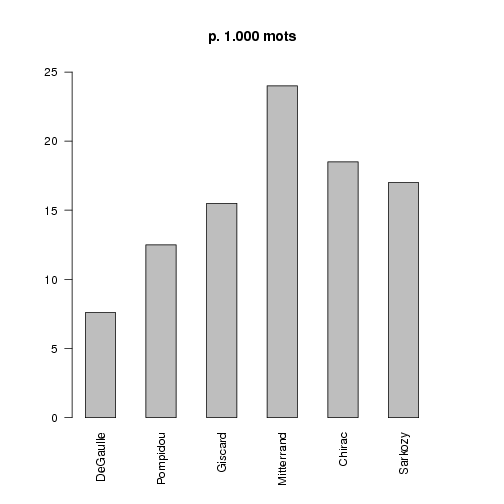
\includegraphics[height=2.5in]{_media/french/je_freq.png} 
%  \caption{Fréquence d'utilisation du mot «~Je~» dans les discours des Présidents de la République Française successifs}
%  \label{fig:je_stats}
%\end{center}
%\end{figure*}
%
Les Français aiment aussi jouer avec leur langue. On peut se référer à
l'Oulipo~\cite{oulipo}, au verlan~\cite{plenat95}, au
Slam~\cite{slam} ou plus généralement à l'usage de la langue
française dans les arts~\cite{arts}. Jean Véronis, chercheur en
traitement automatique des langues, a obtenu un énorme succès avec un
blog~\cite{veronis} intitulé «~Technologies du Langage~» consacré à
l'analyse linguistique dans divers domaines, et surtout en
politique, qui a été classé 1\raise+.5ex\hbox{er} blog scientifique en
France en 2011, et comprend des données intéressantes telles que
l'étude de la langue des hommes politiques français (voir
figure \ref{fig:je_stats}).



\subsection{Le français dans le cyberespace}

Le français est désormais très présent sur Internet, et était classé
8\raise+.5ex\hbox{ème} fin 2009 (voir figure \ref{fig:internettop10})
avec 57 millions d'internautes dans le monde qui le pratiquent~\cite{internettop10}.
%
\begin{figure*}[t]
\begin{center}
 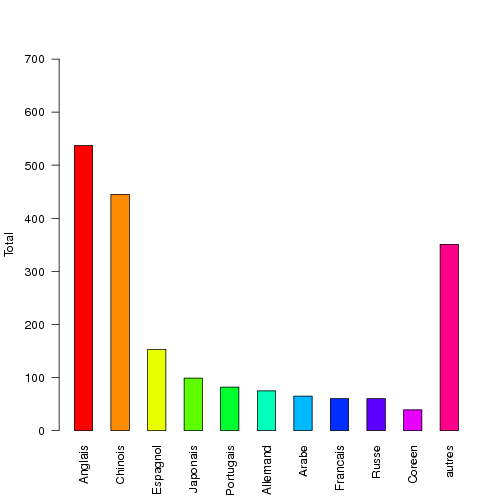
\includegraphics[height=4.0in]{_media/french/french_pix2_top_10_Internet_languages_2010.png}
  \caption{Les 10 langues les plus pratiquées sur Internet fin 2009 (en millions d'usagers)~\cite{internettop10}}
  \label{fig:internettop10}
\end{center}
\end{figure*}

Le français est très actif et présent dans les projets encyclopédiques participatifs comme Wikipedia (1,19 M d'articles en janvier 2012), juste derrière l'allemand ((1,34 M d'articles) mais loin derrière l'anglais (3,84 M d'articles)~\cite{wikipediastats}.

Une loi sur l'accessibilité a été votée en 2005 qui rend
obligatoire de fournir un accès à l'information pour les
personnes handicapées, avec une extension à l'information
numérique (e-Accessibilité) en 2009~\cite{loi}. Cela nécessiterait
l'utilisation de technologies de la langue transmédia, comme
la synthèse vocale pour les aveugles, ou la génération en Langue des
Signes pour les sourds.

\subsection{Quel est le poids du français~?}

Plusieurs études ont été menées sur la place de la langue française
dans le monde. Dans l'ouvrage {\em Le poids des
  Langues}~\cite{calvet09}, A. Calvet et L.J. Calvet proposent de
définir un indice de mesure de ce poids, qui pourrait inclure le
nombre de locuteurs, en première ou deuxième langue, le nombre de
locuteurs étrangers, le nombre de pays où elle est une des langues
officielles, le nombre de traductions (en tant que langue source ou
langue cible), sa présence sur le cyberespace (contenu et accès), mais
aussi le nombre de livres publiés ou le nombre de prix Nobel de
littérature. Sans surprise, le français obtient un bon classement en
fonction de cet indice, juste derrière l'anglais.

\subsection{Pas de multilinguisme sans Technologies de la Langue}

Le français a le statut de langue internationale, même s'il a
perdu beaucoup de sa suprématie avec la prépondérance croissante de
l'anglais (ou du globish (Global English)) comme «~lingua franca~» (!)
internationale. Le français apparaît encore comme une langue
officielle dans de nombreux pays et de nombreuses organisations
internationales. Cependant, avec la mondialisation, la suprématie de
l'anglais peut conduire à une position monopolistique dans
l'économie et la culture, qui aurait de fortes conséquences
politiques. De nombreuses réunions ont maintenant lieu en anglais, et
de nombreux documents sont produits uniquement en anglais. Certains
groupes industriels français demandent à leurs employés de parler 
et d'écrire en anglais, et certains cours dans l'enseignement supérieur sont enseignés en anglais. Le salut du
français, comme pour de nombreuses autres langues, passe par le
multilinguisme, qui peut dans le même temps préserver les cultures
individuelles et permettre de communiquer entre personnes parlant
des langues différentes. Cependant, le coût du multilinguisme est
énorme, tant en termes de financement qu'en termes de charge
de travail. Les technologies de la langue apparaissent comme le seul
moyen de permettre le multilinguisme, en réduisant ces coûts et cette 
charge de travail, et de sauver les langues menacées, dont le français
à long terme.

\subsection{La langue française dans le monde}
\label{frenchInTheWorld}
Le français est parlé dans de nombreux pays autour du
monde~\cite{francaisautourmonde}.

\begin{center}
{\bf {\sc Europe}}
\end{center}

{\bf Andorre}\\
Le catalan est la seule langue officielle d'Andorre; cependant
le français est couramment utilisé du fait de la proximité de la
France.

{\bf Belgique}\\
En Belgique, le français est la langue officielle du Pays Wallon (à
l'exclusion des canton de l'Est, qui parlent allemand)
et une des deux langues officielles (avec le flamand) de la région
Bruxelles-Capitale.

{\bf Italie}\\
Le français est une des deux langues officielles, avec l'Italien, de la petite région de la Vallée d'Aoste en
Italie.

{\bf Luxembourg}\\
Le français est une des trois langues officielles du Grand Duché de
Luxembourg, à côté de l'Allemand et du Luxembourgeois.

{\bf Monaco}\\ 
Bien que le monégasque soit la langue nationale de la Principauté de
Monaco, le français est la seule langue officielle.

{\bf Suisse}\\
Le français est l'une des quatre langues officielles de la
Suisse (avec l'allemand, l'italien et le romanche).

{\bf Le Royaume Uni et les Iles  anglo-normandes}\\
Le français est la langue officielle à Jersey comme à Guernesey.
\vspace{1.0in}
\begin{center}
{\sc Amérique du Nord et du Sud}
\end{center}

{\bf Canada}\\
Le français est la deuxième langue la plus répandue au Canada, après
l'anglais, et les deux sont des langues officielles au niveau
fédéral. Le français est la seule langue officielle dans la province
du Québec, où elle est la langue maternelle de quelque 6 millions de
personnes. Le Nouveau-Brunswick, où environ un tiers de la population
est francophone, est la seule province officiellement bilingue. Des
portions de l'Est et du Nord-Est de l'Ontario, la
Nouvelle-Écosse et le Manitoba ont d'importantes minorités françaises,
mais son statut comme langue officielle dans ces provinces et le
niveau des services francophones varient. De petites poches de
locuteurs français existent dans toutes les autres provinces.

{\bf Haïti}\\
Le français est l'une des deux langues officielles d'Haïti, avec le créole haïtien.

{\bf Départements et Territoires français d'Outre Mer en Amérique}\\
Le français est la langue officielle des départements et territoires
français d'Outre Mer: Guyane française, Guadeloupe,
Martinique, Saint Barthélemy, Saint Martin et Saint-Pierre et
Miquelon.

{\bf États-Unis}\\
Le français est la quatrième langue la plus parlée aux États-Unis,
après l'anglais, l'espagnol et le chinois, et la
seconde langue la plus parlée dans les états de Louisiane, du Maine,
du Vermont et du New Hampshire. La Louisiane est le foyer de nombreux
dialectes distincts, dont le français cajun a le plus grand nombre de
locuteurs. Selon le recensement américain de 2000, il y a plus de
194.000 personnes en Louisiane qui parlent français à la maison.

{\bf Brésil}\\
La langue française était parlée au Brésil, pendant une brève période,
lors des tentatives coloniales de la France en Antarctique et en
France équinoctiale (Guyane). Aujourd'hui, la communauté indigène
Karipuna (près de 30.000 personnes) d'Amapá, au nord du Brésil
parle un créole français, le Lanc-Patua, éventuellement lié à la
langue créole de Guyane française.

\begin{center}
{\sc Afrique}
\end{center}

Une majorité de la population mondiale d'expression française
vit en Afrique. Selon le rapport 2007 de l'Organisation
Internationale de la Francophonie, quelques 115 millions de personnes
dans 31 pays africains francophones peuvent s'exprimer en
français en tant que première ou deuxième langue. En raison de la
hausse de l'usage du français en Afrique, la population totale de langue
française devrait atteindre 700 millions de personnes en 2050.

Le français est une langue officielle dans de nombreux pays africains,
la plupart des anciennes colonies françaises ou belges: Bénin, Burkina
Faso, Burundi, Cameroun, République centrafricaine, Tchad, Comores,
République du Congo, Côte d'Ivoire, République démocratique du
Congo, Djibouti, Guinée équatoriale, Gabon, Guinée, Madagascar, Mali,
Niger, Rwanda, Sénégal, Seychelles et Togo.

En outre, le français est une langue administrative et couramment
utilisée, mais pas avec un statut officiel, à Maurice et dans les
états du Maghreb: Algérie, Mauritanie, Maroc et Tunisie.

{\bf Départements et Territoires français d'Outre Mer en Afrique}\\
Le français est aussi la langue officielle de Mayotte et de La
Réunion, deux territoires d'outre-mer de la France situés dans
le Sud-Ouest de l'Océan Indien.

\begin{center}
{\sc Asie}
\end{center}

{\bf Asie du Sud-Ouest}\\ 
L'arabe est la langue officielle du Liban, alors qu'une 
loi spéciale réglemente l'usage du français. Le
français est considéré comme une langue seconde par le peuple libanais
et est largement utilisé, notamment à des fins administratives. Il est
enseigné dans de nombreuses écoles comme langue seconde avec l'arabe et l'anglais. Comme au Liban, le français était
langue officielle en Syrie jusqu'en 1943. Il y a aussi un
nombre important de personnes parlant français dont c'est la
langue maternelle ou la langue seconde.

{\bf Asie du Sud-Est}\\ 
Le français est une langue administrative au
Laos et au Cambodge, bien que son influence ait décliné au cours de
ces dernières années. Dans le Vietnam colonial, les élites parlaient
français, et beaucoup de ceux qui travaillaient pour les Français
parlaient un créole français connu sous le nom de «~Tây~Boi~»
(aujourd'hui disparu).  Dans le sud de la Chine, le français
était également parlée par l'élite dans le territoire du
Guangzhouwan, loué à la France.

{\bf Inde}\\
Le français a un statut officiel {\em de jure} dans le territoire de l'Union indienne de Pondichéry, avec les langues régionales tamoul
et telugu. Le français est également enseigné dans les écoles de
Chandernagor (une ancienne colonie française dans le Bengale
occidental).

\begin{center}
{\sc Océanie/Australasie}
\end{center}
Le français est une langue officielle de la nation de Vanuatu dans les
îles du Pacifique, où 45\% de la population peut s'exprimer en
français. Dans le territoire français de Nouvelle-Calédonie, 97\% de
la population peut parler, lire et écrire le français. Dans le
territoire français de Wallis et Futuna, 78\% de la population peut
parler, lire et écrire le français.

\subsection{Les langues parlées en France}
\label{languagesSpokenInTheFrance}
De nombreuses langues sont parlées en France~\cite{languesparleesfrance}.

{\bf France métropolitaine}\\
{\em Langues Régionales}~: Alsacien, Basque, Breton, Catalan, Corse, Flamand occidental, Francique mosellan, Franco-provençal, Langues d'oïl (Franc-comtois, Wallon, Champenois, Picard, Normand, Gallo, Poitevin-saintongeais [avec deux variétés~: Poitevin et Saintongeais], Lorrain, Bourguignon-morvandiau), Parlers d'oc ou Occitan (Gascon, Languedocien, Provençal, Auvergnat, Limousin, Vivaro-alpin).

{\em Langues non-territoriales}~: Arabe dialectal, Arménien occidental, Berbère, Judéo-Espagnol, Romani, Yiddish.

{\bf Outre-Mer}\\
\textbf{ \emph{Zone caribéenne}}~:\\
{\em Créole à base lexicale française}~: Guadeloupéen, Guyanais, Martiniquais.
{\em Créole bushinenge en Guyane (à base lexicale anglo-portugaise)}~: Saramaca, Aluku, Njuka, Paramaca.
{\em Langues amérindiennes en Guyane}~: Galibi (ou Kalina), Wayana, Palikur, Arawak (ou Iokono), Wayampi, Emerillon ; Hmong.

{\bf La Réunion}~:\\
Créole réunionnais (à base lexicale française).

{\bf Nouvelle Calédonie}~:\\
28 langues kanaks.\\
{\em Grande Terre}~: Nyelâyu, Kumak, Caac, Yuaga, Jawe, Nemi, Fwâi, Pije, Pwaamei, Pwapwâ, langue Voh-Koné, Cèmuhi, Paicî, Ajië, Arhâ, Arhö, ôrôwe, Neku, Sîchë, Tîrî, Xârâcùù, Xaragurè, Drubéa, Numèè. \\
{\em Iles Loyauté}~: Nengone, Drehu, Iaai, Fagauvea.

{\bf Polynésie française}~:\\
Tahitien, Marquisien, langues de Tuamotu, langue Mangarévienne, langues des Iles Australes: langue Ra'ivavae, Rapa, Ruturu.

{\bf Iles Wallis et Futuna}~:\\
Wallisien, Futunien.

{\bf Mayotte}~:\\
Mahorais, Malgache de Mayotte.

{\bf Langue des signes française (LSF)}\\

\end{multicols}

\clearpage

\ssection[Les Technologies de la Langue pour le français]{Les Technologies de la Langue pour le français}

\begin{multicols}{2}

\subsection{Les Technologies de la Langue}

Les technologies de la langue sont des technologies de l'information
qui sont spécialisées pour traiter le langage humain. Par conséquent,
ces technologies sont souvent regroupées sous le terme de «~technologies
du langage humain~». Le langage humain est produit sous forme orale,
écrite ou signée. Alors que la parole est le mode le plus ancien et le
plus naturel de communication langagière, une information complexe et
la plupart des connaissances humaines sont maintenues et transmises
dans des textes écrits. Les technologies de la langue écrite et orale
traitent ou produisent le langage dans ces deux modes de
réalisation. Mais la langue a aussi des aspects qui sont partagés pour
la parole et le texte comme les dictionnaires, la plus grande partie
de la grammaire ou le sens des énoncés. Ainsi une grande partie des
technologies de la langue ne peut être subsumée sous forme de
traitement de la parole ou du texte. Parmi celles-ci sont les
technologies qui lient la langue et la connaissance. La figure
\ref{fig:languagetechno} illustre le paysage des technologies de la
langue. Pour communiquer, nous mélangeons la langue avec d'autres
modes de communication et d'autres médias d'information. Nous
combinons la parole avec les gestes et les expressions faciales. Les
textes numériques sont combinés avec des images et des sons. Les films
font apparaître la langue sous sa forme parlée et écrite. Ainsi les
technologies de la parole et du texte se chevauchent et interagissent
avec de nombreuses autres technologies qui facilitent le traitement de
la communication multimodale et des documents multimédias.  La langue
des signes permet la communication des personnes atteintes de surdité.

\begin{figure*}[!ht]
 \colorrule{grey3}{\textwidth}{1.5pt}

\begin{center}
 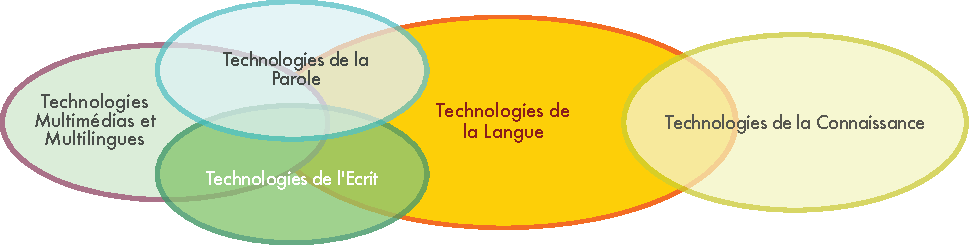
\includegraphics[width=\textwidth]{../_media/french/language_technologies} 
\caption{Les technologies de la langue}
\label{fig:languagetechno}
\end{center}
\vspace*{-.2cm}
 \colorrule{grey3}{\textwidth}{1.5pt}
\end{figure*}

% \begin{figure*}[htb]
%   \colorrule{grey3}{\textwidth}{1.5pt}
%   \center
%   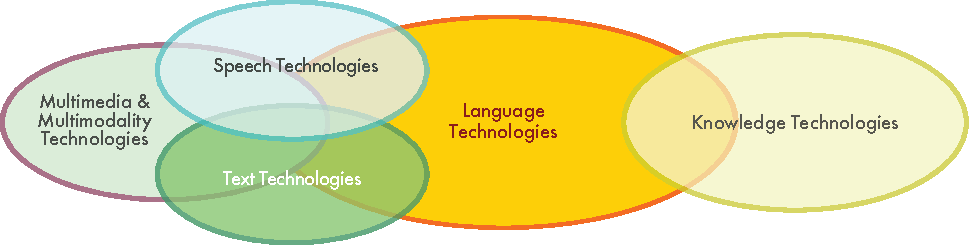
\includegraphics[width=\textwidth]{../_media/english/language_technologies}
%   \caption{Language technologies}
%   \label{fig:ltincontext_en}
%   \colorrule{grey3}{\textwidth}{1.5pt}
% \end{figure*}


\subsection{Les architectures des applications en Technologies de la Langue}

Les applications logicielles typiques du traitement du langage
consistent en plusieurs éléments qui reflètent les différents aspects
de la langue et de la tâche qu'ils mettent en œuvre. La figure \ref{fig:textprocarchi}  
 affiche une architecture très simplifiée que l'on peut trouver
dans un système d'analyse de texte. Les trois premiers modules
traitent de la structure et de la signification du texte en entrée~:
\begin{itemize}
\item Prétraitement: nettoyage des données, en supprimant le
  formatage, détection de la langue d'entrée, etc.

\item Analyse grammaticale: trouver le verbe et ses objets,
  modifieurs, etc. ; détecter la structure de la phrase.

\item Analyse sémantique: désambiguïsation (quel est le bons sens de
  «~pomme~», suivant le contexte~?), résolution d'anaphores et
  d'expressions référentielles comme «~elle~», «~la voiture~», etc.;
  représentation du sens des énoncés d'une manière lisible par une
  machine.
\end{itemize}

Des modules spécifiques à la tâche effectuent alors différentes
opérations telles que le résumé automatique d'un texte, la
consultation d'une base de données et bien d'autres. Nous allons
illustrer ci-dessous les domaines d'application génériques et mettre
en évidence leurs modules de base. Encore une fois, les architectures
des applications sont très simplifiées et idéalisées, pour illustrer
la complexité des applications des technologies de la langue de
manière compréhensible.

Après avoir présenté les domaines d'application de base, nous
donnerons un bref aperçu de la situation concernant les technologies
de la langue pour le français, avec un aperçu des programmes de
recherche passés et en cours. À la fin de cette section, nous
présentons une estimation de la situation concernant les outils de
base et les ressources selon un certain nombre de critères tels que la
disponibilité, la maturité, ou la qualité. Ce tableau vise à donner un
aperçu brut et global de la situation des technologies de la langue
pour le français.

\subsection{Domaines d'application génériques}
%
\subsubsection{Correcteur de texte}
%
Toute personne utilisant un outil de traitement de texte comme
Microsoft Word a fait usage d'un outil de vérification orthographique
qui indique les erreurs d'orthographe et propose des corrections.  40
ans après la sortie du premier programme de correction orthographique
conçu par Ralph Gorin, les correcteurs orthographiques d'aujourd'hui
(voir la figure \ref{fig:spellchecker}) ne se contentent pas de
comparer la liste des mots extraits par rapport à un dictionnaire de
mots correctement orthographiés, mais sont devenus plus
sophistiqués. En plus des algorithmes dépendants de la langue pour
traiter {\bf la morphologie} (formation du pluriel, par exemple),
certains sont maintenant capables de reconnaître des erreurs de
syntaxe simples, comme un verbe manquant ou un verbe qui n'est pas en
accord avec son sujet en personne ou en nombre; par exemple, dans
«~Elle *écris une lettre~».

\begin{figure*}[t]
\colorrule{grey3}{\textwidth}{1.5pt}
\begin{center}
 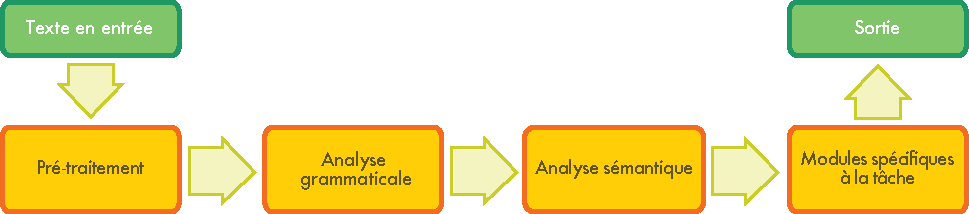
\includegraphics[width=\textwidth]{../_media/french/text_processing_app_architecture}
\caption{Architecture type pour une chaîne de traitement textuel}
\label{fig:textprocarchi}
\end{center}
 \colorrule{grey3}{\textwidth}{1.5pt}
\end{figure*}

Cependant, pour d'autres types d'erreurs communes, les
méthodes actuellement utilisées ne sont pas suffisantes. Prenons par
exemple le premier verset d'un poème de Jerrold H. Zar
(1992)~:\\
\begin{quote}
%\begin{center}
{\em Eye have a spelling chequer,\\
It came with my Pea Sea.\\
It plane lee marks four my revue\\
Miss Steaks I can knot sea.}\\
%\end{center}
\end{quote}
La plupart des correcteurs orthographiques disponibles (y compris MS
Word) ne trouveront pas d'erreurs dans ce poème, car ils ont surtout
regardé les mots isolément. Toutefois, pour détecter les erreurs que
l'on appelle homophones (par exemple «~Eye~» au lieu de «~I~»), le
vérificateur de la langue doit prendre en considération le contexte
dans lequel survient le mot.

\begin{figure*}[t]
\colorrule{grey3}{\textwidth}{1.5pt}
\begin{center}
  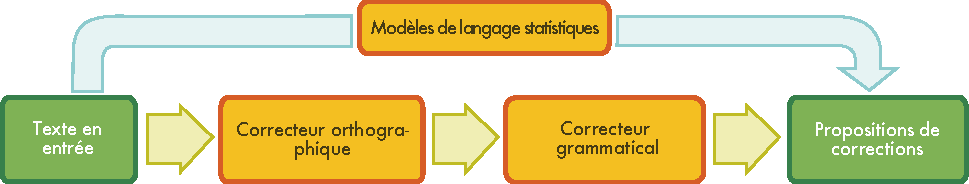
\includegraphics[width=\textwidth]{../_media/french/language_checking.pdf}
\caption{Architecture type de correcteur de texte, à base de règles
  (flèches jaunes) ou statistique (flèche bleue)}
\label{fig:spellchecker}
\end{center}
\colorrule{grey3}{\textwidth}{1.5pt}
\end{figure*}

Ceci nécessite soit la formulation {\bf de règles
de grammaire} spécifiques à la langue, c'est-à-dire à un degré élevé d'expertise et de travail
manuel, soit l'utilisation d'un {\bf modèle de langage statistique} pour
calculer la probabilité d'un mot particulier en fonction des mots
précédents et suivants. Pour une approche statistique, généralement
basée sur des n-grammes, une grande quantité de données linguistiques
(donc {\bf un corpus}) est nécessaire pour obtenir suffisamment de données
statistiques.

Jusqu'à présent, ces approches ont surtout été développées et évaluées
sur des données en langue anglaise. Cependant, elles ne sont pas
nécessairement facilement transférables vers d'autres langues, par
exemple celles qui sont très flexionnelles ou les langues autorisant
une certaine liberté dans l'ordre des mots comme l'allemand. Pour ces langues
plus complexes, un correcteur orthographique avancé de haute précision
peut exiger le développement de méthodes plus sophistiquées,
impliquant une analyse linguistique plus profonde.

L'utilisation de correcteurs n'est pas limitée aux outils de
traitement de texte; ils sont également utilisés dans {\bf les systèmes
d'aide aux auteurs}, c'est-à-dire dans des environnements logiciels où
des manuels et autres documents sont écrits dans des formats
standardisés dans les domaines de l'informatique, de la santé, de
l'ingénierie et des produits en général. Parce qu'elles craignent les
réclamations de leurs clients relatives à une utilisation incorrecte
et les poursuites pour des dommages liés à un mode d'emploi peu
compréhensible, les sociétés sont de plus en plus attentives à la
qualité de leur documentation technique, tout en visant un marché
international à l'aide de la traduction ou de la localisation. Les
avancées du traitement du langage naturel ont conduit au développement
de logiciels de soutien aux auteurs qui aident le rédacteur de
documentation à utiliser un vocabulaire et des structures de phrases
qui soient en accord avec les règles de l'industrie et ses
contraintes terminologiques, ou qui soient simples à comprendre par un
étranger ou bien faciles à traduire.

A côté du traitement de texte et de l'aide aux auteurs, les
correcteurs servent aussi dans le domaine de l'apprentissage des
langues assisté par ordinateur. Ils sont également appliqués aux
requêtes pour les corriger automatiquement et les envoyer aux moteurs
de recherche (voir les suggestions «{\textit{Did you mean ...?}}» de
Google).

En France, la société Synapse Développement commercialise un
correcteur orthographique et grammatical de bonne qualité pour le
français (Cordial, qui est aussi en ligne sur le site de Reverso). Il
existe aussi les correcteurs Antidote de Druide Informatique et
Prolexis des Éditions Diagonal.

\subsubsection{Recherche sur le Web}
Le moteur de recherche (voir la figure \ref{fig:archiweb} pour une
architecture type) de Google, qui a été lancé en 1998, est aujourd'hui 
utilisé pour environ 80\% de toutes les requêtes de recherche
dans le monde entier~\cite{googleworld}, et est également très
populaire en France. Ni l'interface de recherche, ni la présentation
des résultats récupérés n'ont considérablement changé depuis la
première version. Dans la version actuelle, Google propose une
correction orthographique pour les mots mal orthographiés et aussi,
depuis 2009, incorpore des fonctionnalités de recherche sémantique
dans leur mélange algorithmique~\cite{googlesemantics}, ce qui peut
améliorer la précision de la recherche en analysant le sens des termes
de la requête dans son contexte. L'histoire du succès de Google montre
que, avec beaucoup de données à portée de main et des techniques
efficaces pour {\bf l'indexation} de ces données, une approche
essentiellement statistique peut conduire à des résultats
satisfaisants.

Cependant, pour un besoin d'information plus sophistiqué, intégrer des
connaissances linguistiques plus profondes est essentiel. En
particulier, si une requête de recherche se compose d'une question ou
d'une phrase complète, plutôt que d'une liste de mots-clés, la
récupération des réponses pertinentes à cette requête nécessite une
analyse de cette question ou de cette phrase sur un plan syntaxique et
sémantique ainsi que la disponibilité d'un index qui permette une
récupération rapide des documents pertinents.

\begin{figure*}[t]
 \colorrule{grey3}{\textwidth}{1.5pt}
\begin{center}
 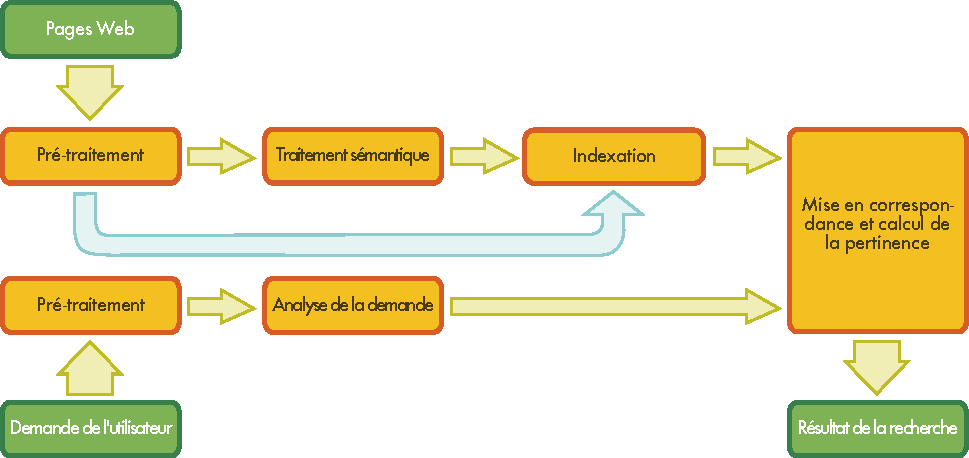
\includegraphics[width=\textwidth]{../_media/french/web_search_architecture}
 \caption{Architecture type de moteur de recherche Web}
\label{fig:archiweb}
\end{center}
 \colorrule{grey3}{\textwidth}{1.5pt}
\end{figure*}

Imaginez par exemple un utilisateur qui saisit la requête «~Donne-moi
une liste de toutes les entreprises qui ont été reprises par d'autres
sociétés au cours des cinq dernières années~». Une simple approche
fondée sur les mots-clés ne nous mènera pas très loin.

Élargir les termes de la requête à l'aide de synonymes, par exemple en
utilisant une ressource linguistique ontologique comme le WordNet de
l'université de Princeton, peut améliorer les résultats. Cependant, pour obtenir une
réponse satisfaisante, {\bf une analyse} plus approfondie {\bf de la requête} est
nécessaire. Par exemple, en appliquant un analyseur syntaxique pour
analyser la structure grammaticale de la phrase, nous pouvons
déterminer que l'utilisateur est à la recherche d'entreprises qui en
ont racheté d'autres et non d'entreprises qui ont été rachetées. Nous
avons également besoin de traiter l'expression «~les cinq dernières
  années~» pour savoir à quelles années elle réfère.

Enfin, la requête doit être traitée en correspondance avec une
quantité massive de données non structurées afin de trouver
l'information ou des éléments d'information que l'utilisateur
cherche. Cela implique {\bf l'obtention} et {\bf le classement} des documents
pertinents. En outre, pour générer une liste d'entreprises, nous avons
également besoin d'extraire l'information qu'une chaîne particulière
de mots dans un document se réfère à un nom de société. Ce genre
d'information est étiqueté en utilisant un système de reconnaissance
d'{\bf Entités Nommées}.

Nous faisons face à un défi supplémentaire si nous voulons faire
correspondre une requête aux documents rédigés dans une langue
différente. Pour {\bf une recherche interlingue}, nous devons traduire
automatiquement la requête dans toutes les langues sources possibles
et cartographier les informations récupérées en retour dans la langue
cible. Encore une fois, cela nécessite une analyse linguistique de
tous les textes impliqués.

Pour les utilisateurs ayant un besoin d'informations très
spécialisées, une expansion de la requête peut nécessiter des
ressources supplémentaires comme des connaissances d'une ontologie
spécifique au domaine, représentant les concepts pertinents dans le
domaine et les relations entre ces concepts.

La part croissante de données disponibles dans des formats non-textuels
entraîne également la demande de services de {\bf recherche multimédia}
permettant, par exemple, de rechercher des informations sur les
images et les données audio et vidéo. Pour les fichiers audio et vidéo, cela
implique un module de {\bf reconnaissance vocale} pour convertir la parole
en texte ou en une représentation phonétique, à laquelle les requêtes
des utilisateurs peuvent être appariées.

En France, la société Exalead a développé avec succès et fait la démonstration en 2010 de 
l'application Voxalead News~\cite{voxaleadnews} de recherche multimédia en 6 langues
(français, anglais, espagnol, chinois mandarin, arabe et russe),
peu de temps avant Google.

\subsubsection{Traitement de la parole}
Le traitement du langage parlé fait partie du traitement des langues,
bien que les communautés travaillant sur la linguistique
computationnelle et sur la communication parlée aient été initialement
séparées, les membres de la première venant de l'informatique
théorique et de l'intelligence artificielle, et les membres de
la seconde venant eux du traitement du signal et de la reconnaissance
des formes.

Les technologies de la langue parlée couvrent de nombreux domaines
différents tels que {\bf l'analyse et la compression de la
  parole, la reconnaissance de la parole et la compréhension, la
  synthèse vocale et la génération, le dialogue oral, la
  reconnaissance du locuteur} (qui parle~?), {\bf l'identification de la langue parlée} (en quelle langue~?). Elles
peuvent être utilisées dans différentes applications : commande
vocale, dictée vocale, transcription de l'audiovisuel, de
conversations ou de réunions, systèmes interactifs, traduction de la
parole, identification des locuteurs, assistance personnelle, etc.

Pour certaines applications, comme les services bancaires par
téléphone, un module de reconnaissance vocale mettant en
correspondance une forme à reconnaître avec celles d'un vocabulaire
existant est suffisant. Pour d'autres applications, par exemple en
dictée vocale ou dans la transcription de conversations, un logiciel
plus sophistiqué ayant la capacité de traiter toute parole naturelle
est nécessaire. Pour les systèmes interactifs avancés, une analyse
linguistique en profondeur de l'entrée vocale s'impose.

\begin{figure*}[!ht]
 \colorrule{grey3}{\textwidth}{1.5pt}
\begin{center}
 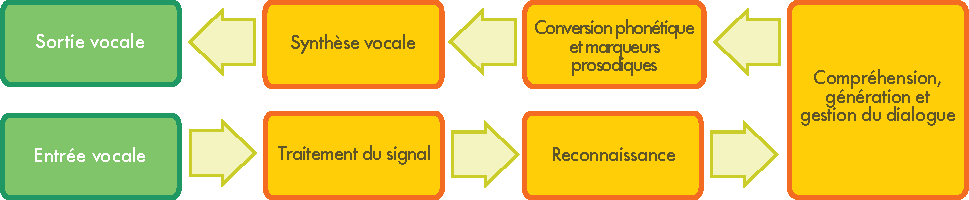
\includegraphics[width=\textwidth]{../_media/french/simple_speech-based_dialogue_architecture} 
\caption{Architecture de base d'un système de dialogue oral}
\label{fig:slds}
\end{center}
 \colorrule{grey3}{\textwidth}{1.5pt}
\end{figure*}

Un système d'interaction vocale complète comprend quatre technologies
différentes (voir figure \ref{fig:slds}):
\begin{itemize}
\item La reconnaissance automatique de la parole (RAP) est chargée de
  déterminer quels mots ont été prononcés, étant donné une
  séquence de sons émis par le locuteur.
\item L'analyse syntaxique et l'interprétation sémantique et
  pragmatique ont pour objet d'analyser la structure syntaxique de
  l'énoncé d'un utilisateur et d'interpréter ce dernier en fonction
  des besoins de l'application.
\item La gestion du dialogue est nécessaire pour déterminer l'action
  qui doit être prise par le système compte tenu de l'entrée de
  l'utilisateur et des fonctionnalités du système.
\item La technologie de synthèse vocale est utilisée pour transformer
  un message en sons qui seront produits pour l'auditeur.
\end{itemize}

Les systèmes de RAP pour une langue donnée sont généralement basés sur
{\bf un modèle acoustique}, qui représente le signal correspondant aux
phonèmes de cette langue, {\bf un modèle de prononciation},
représentant les différentes façons de prononcer les mots de cette
langue, et {\bf un modèle de langage}, qui représente la façon dont
les mots sont ordonnés pour produire des phrases dans cette
langue. Les systèmes de RAP basés sur des approches d'apprentissage statistique nécessitent d'être entraînés sur
de vastes quantités de données (parole transcrite à partir de
différents intervenants avec des accents divers et énormes quantités
de textes reflétant l'application ciblée) pour obtenir des
performances suffisantes.

En dépit d'avancées technologiques majeures dans les années récentes,
les systèmes de RAP actuellement disponibles sont encore confrontés à
des difficultés avec {\bf les mots hors vocabulaire} (MHV) : mots
inconnus du système qui font que les phrases dans lesquelles ils sont
prononcés ne sont pas correctement traitées. Le vocabulaire et le
modèle de langage doivent donc être continuellement mis à jour. Un
autre problème est la difficulté pour un système de reconnaissance
vocale, tout comme pour d'autres technologies de la langue,
d'estimer s'il peut avoir mal compris un mot ou une phrase. Ce
problème peut être résolu en attribuant une mesure de confiance à
chaque mot et phrase reconnus.

Le taux de précision attendu du module de reconnaissance est très
dépendant de l'application. Alors que l'utilisateur d'un système de
dictée vocale peut généralement vérifier manuellement et modifier la
sortie du système, des exigences plus complexes sont imposées à un
système de dialogue destiné à converser naturellement avec un
humain. Cela implique~: 
\begin{itemize}
\item une analyse linguistique profonde de l'entrée vocale
  (reconnaissance d'Entités Nommées, analyse morpho-syntaxique,
  résolution des coréférences, analyse syntaxique),
\item mais aussi une composante de {\bf gestion de dialogue}, qui
  utilise les connaissances du domaine spécifique de la tâche pour
  analyser l'entrée, à un niveau sémantique et pragmatique, afin de
  générer la sortie appropriée,
\item et même {\bf l'analyse et la génération des émotions}, à
  travers le traitement de la prosodie (rythme, accent et intonation),
\item sans oublier l'analyse des autres {\bf modalités non-verbales}
  (regard, gestes, expression faciale, etc.).
\end{itemize}

La seule façon d'évaluer la qualité d'un système de RAP est de mener
une {\bf évaluation} sur des données de test correspondant à
l'application. Plusieurs systèmes basés sur des approches différentes
peuvent être comparés dans {\bf des campagnes d'évaluation}, telles
que celles organisées aux États-Unis par le NIST (National Institute
of Standards and Technology) pour la DARPA (Defense Advanced Research
Projects Agency) depuis 1987.

Le tableau de la figure \ref{fig:nistreco} montre les progrès réalisés
par les systèmes de reconnaissance automatiques de la parole au fil
des ans, à travers les campagnes d'évaluation internationales
menées par le NIST. Apparaît sur ce tableau la meilleure performance
obtenue cette année-là, en termes de {\bf taux d'erreur sur
  les mots} (WER) selon une échelle logarithmique (l'effort
pour passer de 100\% d'erreurs (le système ne reconnaît
correctement aucun mot) à 10\% d'erreurs étant comparable à
celui requis pour passer de 10\% à 1\% d'erreurs). Les tâches
deviennent de plus en plus difficiles au fil des années (d'abord avec un langage de commande vocale artificiel de 1000 mots,
puis pour la dictée vocale (20 000 mots), la transcription d'émissions de radio ou de télévision (anglais, arabe et chinois
mandarin), la transcription de conversations téléphoniques (également
en anglais, arabe et mandarin), la transcription de réunions, etc.),
dans des conditions variables (temps réel ou non, différentes qualités
de prise de son, etc.). Nous voyons que pour certaines tâches, les
performances des systèmes sont semblables à celles d'un
auditeur humain, ce qui rend ces systèmes exploitables et
commercialisables (pour des langages de commande, par exemple). Par
contre, il est clair que pour des tâches plus complexes, les
performances s'améliorent plus lentement, justifiant la
poursuite de l'effort de recherche. La connaissance de ces
performances est précieuse pour déterminer la faisabilité d'une application sur la base du niveau de qualité qu'elle
requiert. Par exemple, un système de recherche d'information 
sur des données audiovisuelles ne nécessite pas de très hautes
performances dans la transcription de la parole, contrairement à un
système de dialogue oral utilisé pour des tâches critiques.

Transformer un message écrit en un signal de parole est effectué par
un module de {\bf synthèse vocale}. Ce message peut être un texte
({\bf synthèse à partir du texte}) ou la sortie d'un système de dialogue
interactif. Aujourd'hui, la synthèse vocale est généralement basée sur
de grandes quantités de données de parole préenregistrées afin de
produire un résultat raisonnablement naturel. Cependant, si l'on
considère le but ultime de produire automatiquement de la parole
naturelle dans des systèmes interactifs, des recherches
supplémentaires sont nécessaires, en particulier concernant
l'interrelation entre syntaxe, sémantique, pragmatique et prosodie, et
entre les modalités verbales et non verbales (expressions faciales des
{\bf visages parlants}, pointage gestuel, etc.).

\begin{figure*}[!ht]
\begin{center}
  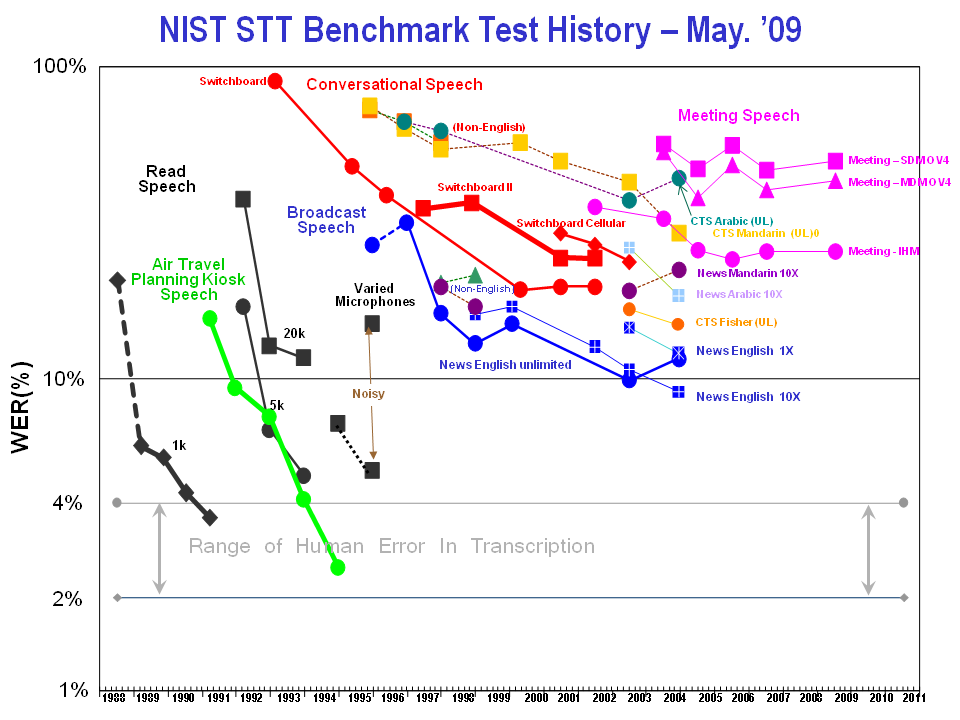
\includegraphics[height=4.0in]{_media/french/french_pix8_speech_reco_nist.png}
  \caption{Une histoire de la Reconnaissance Automatique de la Parole depuis 1987 à travers les campagnes d'évaluation du NIST~\cite{speechreconist}}
  \label{fig:nistreco}
\end{center}
\end{figure*}

La langue française présente des spécificités qui la rendent plus
difficile à traiter par les systèmes automatiques de traitement de la
parole que d'autres langues romanes comme l'italien ou l'espagnol. Les
hétérographes homophones (également appelés homonymes) soulèvent des
problèmes pour la transcription écrite de la parole (transcription
phonème-graphème), et cela est souvent le cas pour la marque du
pluriel en français (``s'' pour les noms, ``nt'' pour les verbes) qui
ne se prononce pas, ou se prononce comme une liaison entre les
mots. Les hétérophones homographes posent des problèmes pour la
conversion graphème-phonème en synthèse à partir du texte, qui peuvent
nécessiter une analyse syntaxique («~Les poules du couvent couvent~»,
prononcé /lepuldykuvãkuv/) voire même une analyse sémantique pour
quelques très rares cas («~fils~» (de famille) prononcé / fis / et
«~fils~» (de soie), prononcé / fil /).

Une question clé pour les recherches futures est {\bf la personnalisation}
des systèmes interactifs. Dans une certaine mesure, cela est déjà
possible, par exemple dans les systèmes de transcription de la parole,
qui peuvent également reconnaître le genre, la tranche d'âge, l'accent
ou l'identité ({\bf diarisation}) de la personne qui parle, et dans les
systèmes de dictée vocale ou les systèmes de navigation automobile,
qui peuvent être entraînés à s'adapter au style de locution de
l'utilisateur. Veiller à doter les systèmes de dialogue d'une ergonomie
conviviale est particulièrement important, par exemple pour les systèmes
d'assistance aux personnes handicapées ou âgées, qui peuvent avoir des
inhibitions contre l'utilisation de systèmes informatiques. Cela
impliquera une analyse du comportement langagier de l'utilisateur en
général, et en particulier de la façon dont les humains interagissent
avec les ordinateurs.

D'autres aspects du traitement de la parole concernent {\bf la vérification
ou l'identification du locuteur}, pour les applications en biométrie,
ou {\bf l'identification de la langue ou du dialecte}, visant à identifier
quelle est la langue qui est parlée.

En ces temps où les marchés européens et internationaux progressent de
concert, un défi important pour les systèmes interactifs est leur
capacité à travailler dans un environnement multilingue, ce qui
implique {\bf la traduction automatique de la parole} dans différentes
langues. Des premiers résultats ont été démontrés en avril 2007, au
sein du projet TC-STAR~\cite{tcstarurl} financé par la Commission
Européenne, pour la traduction de l'anglais vers l'espagnol des discours du Parlement Européen, profitant de l'existence de grandes quantités de corpus parallèles (les
discussions des parlementaires, leurs interprétations dans toutes les
langues officielles de l'UE, leur transcription et la
traduction de leur transcription également dans toutes les langues de
l'UE). La technologie correspondante a été mise en œuvre dans
le système Jibbigo~\cite{jibbigo} disponible en 2011 pour 8 paires de langues
sur l'{\em {\mbox App Store}} d'Apple. Google offre
pour sa part, en 2011, la traduction dans 3300 paires de langues, avec
reconnaissance vocale pour 17 langues sources et synthèse vocale pour
25 langues cibles (dont le français), dans son application Google
Translate pour «~smartphone~» (téléphone intelligent), également
disponible sur l'{\em {\mbox App Store}}.

La qualité de la traduction de parole interactive doit encore être
améliorée avant que son utilisation puisse devenir naturelle. De même,
les systèmes de dialogue oral ne sont actuellement disponibles que
pour des applications très limitées. Cependant, de nombreuses
applications peuvent être abordées avec la technologie actuellement
disponible, telle que {\bf le sous-titrage vidéo automatique} avec une
traduction approximative.

Au-delà de l'état actuel de la technologie, il y aura des
changements significatifs en raison de la propagation des smartphones
comme une nouvelle plate-forme pour la gestion des relations clients -
en plus des canaux téléphoniques, de l'Internet et du courrier
électronique. Cette tendance va également affecter l'utilisation des technologies d'interaction vocale. Alors
que la demande pour la téléphonie basée sur des {\bf interfaces
  vocales avec les utilisateurs} (VUI) va diminuer sur le long terme,
l'usage de la langue parlée en tant que modalité d'entrée conviviale pour les smartphones va prendre une importance
significative. Cette tendance est soutenue par l'amélioration
observable des performances de la reconnaissance vocale multilocuteur
pour les services de dictée ou de commande vocales qui sont déjà
offerts comme des services pour les utilisateurs de smartphones (voir
par exemple Apple Siri ou Android Voice Actions). Compte tenu de cette
«~externalisation~» de la tâche de reconnaissance à l'infrastructure des applications, l'emploi d'une
analyse linguistique spécifique à l'application gagnera en
importance par rapport à la situation actuelle.

\begin{figure*}[t]
 \colorrule{grey3}{\textwidth}{1.5pt}
\begin{center}
 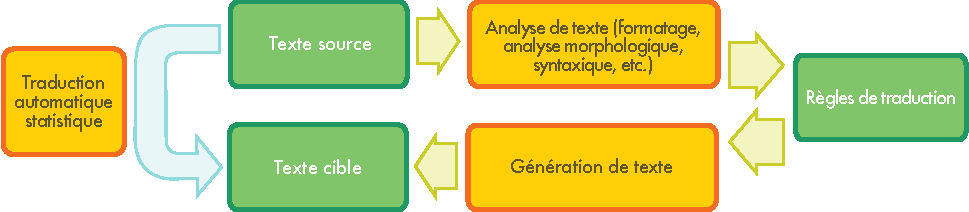
\includegraphics[width=\textwidth]{../_media/french/machine_translation}
\caption{Traduction automatique statistique (flèche bleue) ou à base de règles (flèches jaunes)}
\label{fig:mtarchi}
\end{center}
 \colorrule{grey3}{\textwidth}{1.5pt}
\end{figure*}

\subsubsection{Traduction Automatique}
L'idée d'utiliser des ordinateurs numériques pour la traduction des
langues naturelles est venue en 1946 d'A.D. Booth et a été suivie par
un financement substantiel pour la recherche dans ce domaine dans les
années 1950 et de nouveau dans les années 1980. La France était
particulièrement active dans ce domaine, et le premier livre populaire
sur {\bf la traduction automatique} (TA) a été écrit par un Français
(Delavenay, 1957). Néanmoins, la traduction automatique ne
parvient toujours pas à répondre aux attentes qu'elle a suscitées à
ses débuts.

À son niveau de base, la traduction automatique substitue simplement les mots d'une langue
par les mots d'une autre. Cela peut être utile dans des domaines
possédant un langage formellement très restreint, par exemple les
bulletins météorologiques. Cependant, pour une bonne traduction de
textes moins standardisés, des unités de texte plus larges
(expressions, phrases ou même passages entiers) doivent être adaptées à
leurs plus proches équivalents dans la langue cible. La difficulté
majeure réside dans le fait que le langage humain est ambigu, ce qui
donne des défis à plusieurs niveaux, par exemple, {\bf la
  désambiguïsation du sens des mots} au niveau lexical («~avocat~»
peut signifier un homme de loi ou un fruit) ou le rattachement des phrases prépositionnelles au niveau syntaxique comme dans~:

\begin{tabular}{l}
\\
Le policier observait l'homme avec ses jumelles.\\
$[${\em The policeman observed the man with his binoculars.}$]$\\
Le policier observait l'homme avec son revolver.\\
$[${\em The policeman observed the man with his revolver.}$]$\\
\\
\end{tabular}

Une façon d'aborder la tâche est basée sur des règles
linguistiques (voir figure \ref{fig:mtarchi}). Pour les traductions entre des langues étroitement
apparentées, une traduction directe peut être réalisable dans des cas
comme celui de l'exemple ci-dessus. Mais les systèmes {\bf basés sur  des
règles} (ou {\bf basés sur la connaissance}) analysent souvent le texte
d'entrée et créent une représentation intermédiaire symbolique, à
partir de laquelle le texte est généré dans la langue cible.  Le
succès de ces méthodes est très dépendant de la disponibilité de
lexiques étendus incluant des informations morphologiques, syntaxiques
et sémantiques, et de grands ensembles de règles de {\bf grammaire}
soigneusement conçues par un linguiste qualifié.

Introduits à la fin des années 1980 par des chercheurs issus de la
communauté de la reconnaissance vocale, dans la mesure où la puissance
de calcul s'était accrue et était devenue moins coûteuse, on a noté un
surcroît de l'intérêt des {\bf modèles statistiques} pour la TA. Les
paramètres de ces modèles statistiques sont tirés de l'analyse de
{\bf corpus de textes bilingues}, comme le {\bf corpus parallèle} Europarl, qui
contient les actes du Parlement européen dans 21 langues
européennes. En fonction de la disponibilité d'une quantité suffisante
de données, la traduction automatique statistique fonctionne assez bien pour tirer une
signification approximative d'un texte écrit en langue
étrangère. Cependant, plus que les systèmes fondés sur les règles, les
systèmes de traduction automatique statistiques (ou fondés sur les données) peuvent
générer une sortie agrammaticale. D'autre part, outre l'avantage de
nécessiter moins d'effort humain pour écrire la grammaire, la TA
statistique peut également couvrir les particularités de la langue qui
disparaissent dans les systèmes à base de connaissances, comme par
exemple pour la traduction des expressions idiomatiques.

\begin{figure*}[tbp]
  \centering
  \setlength{\tabcolsep}{0.17em}
  \small
  \begin{tabular}{>{\columncolor{corange1}}cccccccccccccccccccccccc}
    & \multicolumn{22}{>{\columncolor{corange1}}c}{\textcolor{red}{Langues cibles (abscisse)} -- \textcolor{grey1}{Langues sources (ordonnée)}}\\\addlinespace[{-.009cm}]
    \rowcolor{corange1}  & EN & BG & DE & CS & DA & EL & ES & ET & FI & FR & HU & IT & LT & LV & MT & NL & PL & PT & RO & SK & SL & SV\\
    EN & -- & \textcolor{blue}{40.5} & \textcolor{blue}{46.8} & \textcolor{green2}{52.6} & \textcolor{green2}{50.0} & \textcolor{blue}{41.0} & \textcolor{green2}{55.2} & \textcolor{purple}{34.8} & \textcolor{purple}{38.6} & \textcolor{green2}{50.1} & \textcolor{purple}{37.2} & \textcolor{green2}{50.4} & \textcolor{purple}{39.6} & \textcolor{blue}{43.4} & \textcolor{purple}{39.8} & \textcolor{green2}{52.3} & \textcolor{blue}{49.2} & \textcolor{green2}{55.0} & \textcolor{blue}{49.0} & \textcolor{blue}{44.7} & \textcolor{green2}{50.7} & \textcolor{green2}{52.0}\\
    BG & \textcolor{green}{61.3} & -- & \textcolor{purple}{38.7} & \textcolor{purple}{39.4} & \textcolor{purple}{39.6} & \textcolor{purple}{34.5} & \textcolor{blue}{46.9} & \textcolor{red3}{25.5} & \textcolor{red3}{26.7} & \textcolor{blue}{42.4} & \textcolor{red3}{22.0} & \textcolor{blue}{43.5} & \textcolor{red3}{29.3} & \textcolor{red3}{29.1} & \textcolor{red3}{25.9} & \textcolor{blue}{44.9} & \textcolor{purple}{35.1} & \textcolor{blue}{45.9} & \textcolor{purple}{36.8} & \textcolor{purple}{34.1} & \textcolor{purple}{34.1} & \textcolor{purple}{39.9}\\
    DE & \textcolor{green2}{53.6} & \textcolor{red3}{26.3} & -- & \textcolor{purple}{35.4} & \textcolor{blue}{43.1} & \textcolor{purple}{32.8} & \textcolor{blue}{47.1} & \textcolor{red3}{26.7} & \textcolor{red3}{29.5} & \textcolor{purple}{39.4} & \textcolor{red3}{27.6} & \textcolor{blue}{42.7} & \textcolor{red3}{27.6} & \textcolor{purple}{30.3} & \textcolor{red2}{19.8} & \textcolor{green2}{50.2} & \textcolor{purple}{30.2} & \textcolor{blue}{44.1} & \textcolor{purple}{30.7} & \textcolor{red3}{29.4} & \textcolor{purple}{31.4} & \textcolor{blue}{41.2}\\
    CS & \textcolor{green2}{58.4} & \textcolor{purple}{32.0} & \textcolor{blue}{42.6} & -- & \textcolor{blue}{43.6} & \textcolor{purple}{34.6} & \textcolor{blue}{48.9} & \textcolor{purple}{30.7} & \textcolor{purple}{30.5} & \textcolor{blue}{41.6} & \textcolor{red3}{27.4} & \textcolor{blue}{44.3} & \textcolor{purple}{34.5} & \textcolor{purple}{35.8} & \textcolor{red3}{26.3} & \textcolor{blue}{46.5} & \textcolor{purple}{39.2} & \textcolor{blue}{45.7} & \textcolor{purple}{36.5} & \textcolor{blue}{43.6} & \textcolor{blue}{41.3} & \textcolor{blue}{42.9}\\
    DA & \textcolor{green2}{57.6} & \textcolor{red3}{28.7} & \textcolor{blue}{44.1} & \textcolor{purple}{35.7} & -- & \textcolor{purple}{34.3} & \textcolor{blue}{47.5} & \textcolor{red3}{27.8} & \textcolor{purple}{31.6} & \textcolor{blue}{41.3} & \textcolor{red3}{24.2} & \textcolor{blue}{43.8} & \textcolor{red3}{29.7} & \textcolor{purple}{32.9} & \textcolor{red3}{21.1} & \textcolor{blue}{48.5} & \textcolor{purple}{34.3} & \textcolor{blue}{45.4} & \textcolor{purple}{33.9} & \textcolor{purple}{33.0} & \textcolor{purple}{36.2} & \textcolor{blue}{47.2}\\
    EL & \textcolor{green2}{59.5} & \textcolor{purple}{32.4} & \textcolor{blue}{43.1} & \textcolor{purple}{37.7} & \textcolor{blue}{44.5} & -- & \textcolor{green2}{54.0} & \textcolor{red3}{26.5} & \textcolor{red3}{29.0} & \textcolor{blue}{48.3} & \textcolor{red3}{23.7} & \textcolor{blue}{49.6} & \textcolor{red3}{29.0} & \textcolor{purple}{32.6} & \textcolor{red3}{23.8} & \textcolor{blue}{48.9} & \textcolor{purple}{34.2} & \textcolor{green2}{52.5} & \textcolor{purple}{37.2} & \textcolor{purple}{33.1} & \textcolor{purple}{36.3} & \textcolor{blue}{43.3}\\
    ES & \textcolor{green}{60.0} & \textcolor{purple}{31.1} & \textcolor{blue}{42.7} & \textcolor{purple}{37.5} & \textcolor{blue}{44.4} & \textcolor{purple}{39.4} & -- & \textcolor{red3}{25.4} & \textcolor{red3}{28.5} & \textcolor{green2}{51.3} & \textcolor{red3}{24.0} & \textcolor{green2}{51.7} & \textcolor{red3}{26.8} & \textcolor{purple}{30.5} & \textcolor{red3}{24.6} & \textcolor{blue}{48.8} & \textcolor{purple}{33.9} & \textcolor{green2}{57.3} & \textcolor{purple}{38.1} & \textcolor{purple}{31.7} & \textcolor{purple}{33.9} & \textcolor{blue}{43.7}\\
    ET & \textcolor{green2}{52.0} & \textcolor{red3}{24.6} & \textcolor{purple}{37.3} & \textcolor{purple}{35.2} & \textcolor{purple}{37.8} & \textcolor{red3}{28.2} & \textcolor{blue}{40.4} & -- & \textcolor{purple}{37.7} & \textcolor{purple}{33.4} & \textcolor{purple}{30.9} & \textcolor{purple}{37.0} & \textcolor{purple}{35.0} & \textcolor{purple}{36.9} & \textcolor{red3}{20.5} & \textcolor{blue}{41.3} & \textcolor{purple}{32.0} & \textcolor{purple}{37.8} & \textcolor{red3}{28.0} & \textcolor{purple}{30.6} & \textcolor{purple}{32.9} & \textcolor{purple}{37.3}\\
    FI & \textcolor{blue}{49.3} & \textcolor{red3}{23.2} & \textcolor{purple}{36.0} & \textcolor{purple}{32.0} & \textcolor{purple}{37.9} & \textcolor{red3}{27.2} & \textcolor{purple}{39.7} & \textcolor{purple}{34.9} & -- & \textcolor{red3}{29.5} & \textcolor{red3}{27.2} & \textcolor{purple}{36.6} & \textcolor{purple}{30.5} & \textcolor{purple}{32.5} & \textcolor{red2}{19.4} & \textcolor{blue}{40.6} & \textcolor{red3}{28.8} & \textcolor{purple}{37.5} & \textcolor{red3}{26.5} & \textcolor{red3}{27.3} & \textcolor{red3}{28.2} & \textcolor{purple}{37.6}\\
    FR & \textcolor{green}{64.0} & \textcolor{purple}{34.5} & \textcolor{blue}{45.1} & \textcolor{purple}{39.5} & \textcolor{blue}{47.4} & \textcolor{blue}{42.8} & \textcolor{green}{60.9} & \textcolor{red3}{26.7} & \textcolor{purple}{30.0} & -- & \textcolor{red3}{25.5} & \textcolor{green2}{56.1} & \textcolor{red3}{28.3} & \textcolor{purple}{31.9} & \textcolor{red3}{25.3} & \textcolor{green2}{51.6} & \textcolor{purple}{35.7} & \textcolor{green}{61.0} & \textcolor{blue}{43.8} & \textcolor{purple}{33.1} & \textcolor{purple}{35.6} & \textcolor{blue}{45.8}\\
    HU & \textcolor{blue}{48.0} & \textcolor{red3}{24.7} & \textcolor{purple}{34.3} & \textcolor{purple}{30.0} & \textcolor{purple}{33.0} & \textcolor{red3}{25.5} & \textcolor{purple}{34.1} & \textcolor{red3}{29.6} & \textcolor{red3}{29.4} & \textcolor{purple}{30.7} & -- & \textcolor{purple}{33.5} & \textcolor{red3}{29.6} & \textcolor{purple}{31.9} & \textcolor{red2}{18.1} & \textcolor{purple}{36.1} & \textcolor{red3}{29.8} & \textcolor{purple}{34.2} & \textcolor{red3}{25.7} & \textcolor{red3}{25.6} & \textcolor{red3}{28.2} & \textcolor{purple}{30.5}\\
    IT & \textcolor{green}{61.0} & \textcolor{purple}{32.1} & \textcolor{blue}{44.3} & \textcolor{purple}{38.9} & \textcolor{blue}{45.8} & \textcolor{blue}{40.6} & \textcolor{red3}{26.9} & \textcolor{red3}{25.0} & \textcolor{red3}{29.7} & \textcolor{green2}{52.7} & \textcolor{red3}{24.2} & -- & \textcolor{red3}{29.4} & \textcolor{purple}{32.6} & \textcolor{red3}{24.6} & \textcolor{green2}{50.5} & \textcolor{purple}{35.2} & \textcolor{green2}{56.5} & \textcolor{purple}{39.3} & \textcolor{purple}{32.5} & \textcolor{purple}{34.7} & \textcolor{blue}{44.3}\\
    LT & \textcolor{green2}{51.8} & \textcolor{red3}{27.6} & \textcolor{purple}{33.9} & \textcolor{purple}{37.0} & \textcolor{purple}{36.8} & \textcolor{red3}{26.5} & \textcolor{red3}{21.1} & \textcolor{purple}{34.2} & \textcolor{purple}{32.0} & \textcolor{purple}{34.4} & \textcolor{red3}{28.5} & \textcolor{purple}{36.8} & -- & \textcolor{blue}{40.1} & \textcolor{red3}{22.2} & \textcolor{purple}{38.1} & \textcolor{purple}{31.6} & \textcolor{purple}{31.6} & \textcolor{red3}{29.3} & \textcolor{purple}{31.8} & \textcolor{purple}{35.3} & \textcolor{purple}{35.3}\\
    LV & \textcolor{green2}{54.0} & \textcolor{red3}{29.1} & \textcolor{purple}{35.0} & \textcolor{purple}{37.8} & \textcolor{purple}{38.5} & \textcolor{red3}{29.7} & \textcolor{red2}{8.0} & \textcolor{purple}{34.2} & \textcolor{purple}{32.4} & \textcolor{purple}{35.6} & \textcolor{red3}{29.3} & \textcolor{purple}{38.9} & \textcolor{purple}{38.4} & -- & \textcolor{red3}{23.3} & \textcolor{blue}{41.5} & \textcolor{purple}{34.4} & \textcolor{purple}{39.6} & \textcolor{purple}{31.0} & \textcolor{purple}{33.3} & \textcolor{purple}{37.1} & \textcolor{purple}{38.0}\\
    MT & \textcolor{green}{72.1} & \textcolor{purple}{32.2} & \textcolor{purple}{37.2} & \textcolor{purple}{37.9} & \textcolor{purple}{38.9} & \textcolor{purple}{33.7} & \textcolor{blue}{48.7} & \textcolor{red3}{26.9} & \textcolor{red3}{25.8} & \textcolor{blue}{42.4} & \textcolor{red3}{22.4} & \textcolor{blue}{43.7} & \textcolor{purple}{30.2} & \textcolor{purple}{33.2} & -- & \textcolor{blue}{44.0} & \textcolor{purple}{37.1} & \textcolor{blue}{45.9} & \textcolor{purple}{38.9} & \textcolor{purple}{35.8} & \textcolor{blue}{40.0} & \textcolor{blue}{41.6}\\
    NL & \textcolor{green2}{56.9} & \textcolor{red3}{29.3} & \textcolor{blue}{46.9} & \textcolor{purple}{37.0} & \textcolor{blue}{45.4} & \textcolor{purple}{35.3} & \textcolor{blue}{49.7} & \textcolor{red3}{27.5} & \textcolor{red3}{29.8} & \textcolor{blue}{43.4} & \textcolor{red3}{25.3} & \textcolor{blue}{44.5} & \textcolor{red3}{28.6} & \textcolor{purple}{31.7} & \textcolor{red3}{22.0} & -- & \textcolor{purple}{32.0} & \textcolor{blue}{47.7} & \textcolor{purple}{33.0} & \textcolor{purple}{30.1} & \textcolor{purple}{34.6} & \textcolor{blue}{43.6}\\
    PL & \textcolor{green}{60.8} & \textcolor{purple}{31.5} & \textcolor{blue}{40.2} & \textcolor{blue}{44.2} & \textcolor{blue}{42.1} & \textcolor{purple}{34.2} & \textcolor{blue}{46.2} & \textcolor{red3}{29.2} & \textcolor{red3}{29.0} & \textcolor{blue}{40.0} & \textcolor{red3}{24.5} & \textcolor{blue}{43.2} & \textcolor{purple}{33.2} & \textcolor{purple}{35.6} & \textcolor{red3}{27.9} & \textcolor{blue}{44.8} & -- & \textcolor{blue}{44.1} & \textcolor{purple}{38.2} & \textcolor{purple}{38.2} & \textcolor{purple}{39.8} & \textcolor{blue}{42.1}\\
    PT & \textcolor{green}{60.7} & \textcolor{purple}{31.4} & \textcolor{blue}{42.9} & \textcolor{purple}{38.4} & \textcolor{blue}{42.8} & \textcolor{blue}{40.2} & \textcolor{green}{60.7} & \textcolor{red3}{26.4} & \textcolor{red3}{29.2} & \textcolor{green2}{53.2} & \textcolor{red3}{23.8} & \textcolor{green2}{52.8} & \textcolor{red3}{28.0} & \textcolor{purple}{31.5} & \textcolor{red3}{24.8} & \textcolor{blue}{49.3} & \textcolor{purple}{34.5} & -- & \textcolor{purple}{39.4} & \textcolor{purple}{32.1} & \textcolor{purple}{34.4} & \textcolor{blue}{43.9}\\
    RO & \textcolor{green}{60.8} & \textcolor{purple}{33.1} & \textcolor{purple}{38.5} & \textcolor{purple}{37.8} & \textcolor{blue}{40.3} & \textcolor{purple}{35.6} & \textcolor{green2}{50.4} & \textcolor{red3}{24.6} & \textcolor{red3}{26.2} & \textcolor{blue}{46.5} & \textcolor{red3}{25.0} & \textcolor{blue}{44.8} & \textcolor{red3}{28.4} & \textcolor{red3}{29.9} & \textcolor{red3}{28.7} & \textcolor{blue}{43.0} & \textcolor{purple}{35.8} & \textcolor{blue}{48.5} & -- & \textcolor{purple}{31.5} & \textcolor{purple}{35.1} & \textcolor{purple}{39.4}\\
    SK & \textcolor{green}{60.8} & \textcolor{purple}{32.6} & \textcolor{purple}{39.4} & \textcolor{blue}{48.1} & \textcolor{blue}{41.0} & \textcolor{purple}{33.3} & \textcolor{blue}{46.2} & \textcolor{red3}{29.8} & \textcolor{red3}{28.4} & \textcolor{purple}{39.4} & \textcolor{red3}{27.4} & \textcolor{blue}{41.8} & \textcolor{purple}{33.8} & \textcolor{purple}{36.7} & \textcolor{red3}{28.5} & \textcolor{blue}{44.4} & \textcolor{purple}{39.0} & \textcolor{blue}{43.3} & \textcolor{purple}{35.3} & -- & \textcolor{blue}{42.6} & \textcolor{blue}{41.8}\\
    SL & \textcolor{green}{61.0} & \textcolor{purple}{33.1} & \textcolor{purple}{37.9} & \textcolor{blue}{43.5} & \textcolor{blue}{42.6} & \textcolor{purple}{34.0} & \textcolor{blue}{47.0} & \textcolor{purple}{31.1} & \textcolor{red3}{28.8} & \textcolor{purple}{38.2} & \textcolor{red3}{25.7} & \textcolor{blue}{42.3} & \textcolor{purple}{34.6} & \textcolor{purple}{37.3} & \textcolor{purple}{30.0} & \textcolor{blue}{45.9} & \textcolor{purple}{38.2} & \textcolor{blue}{44.1} & \textcolor{purple}{35.8} & \textcolor{purple}{38.9} & -- & \textcolor{blue}{42.7}\\
    SV & \textcolor{green2}{58.5} & \textcolor{red3}{26.9} & \textcolor{blue}{41.0} & \textcolor{purple}{35.6} & \textcolor{blue}{46.6} & \textcolor{purple}{33.3} & \textcolor{blue}{46.6} & \textcolor{red3}{27.4} & \textcolor{purple}{30.9} & \textcolor{purple}{38.9} & \textcolor{red3}{22.7} & \textcolor{blue}{42.0} & \textcolor{red3}{28.2} & \textcolor{purple}{31.0} & \textcolor{red3}{23.7} & \textcolor{blue}{45.6} & \textcolor{purple}{32.2} & \textcolor{blue}{44.2} & \textcolor{purple}{32.7} & \textcolor{purple}{31.3} & \textcolor{purple}{33.5} & --\\
    \end{tabular}
%  \caption{Performances (mesure BLEU) de Traduction Automatique pour un ensemble de paires de langues constitué à partir de 22 langues officielles de l'Union Européenne~\cite{mt462}. La langue source est donnée en ligne et la langue cible est donnée en colonne.}
 \caption{Performances des systèmes de Traduction Automatique entre 22 langues de
   l'UE~\cite{mt462}}
 \label{fig:euromatrixplus}
\end{figure*}

Les {\bf approches hybrides} visent à combiner les approches à base de
connaissances et les approches statistiques. Cela peut être fait de
plusieurs façons. L'une consiste à utiliser à la fois les
systèmes à base de connaissances et les systèmes statistiques et à
avoir un module de sélection pour décider de la meilleure sortie pour
chaque phrase. Toutefois, pour des phrases plus longues, aucun
résultat ne sera parfait. Une meilleure solution est de combiner les
meilleures parties de chaque phrase provenant de sorties multiples, ce
qui peut être relativement complexe, dans la mesure où la
correspondance de parties provenant de plusieurs alternatives n'est pas toujours évidente et nécessite un alignement. Une autre
approche en lice est de combiner les avantages des deux paradigmes~;
par exemple, en rendant un système par règle adaptatif par l'ajout d'un module d'apprentissage des règles, ou
en rendant un système statistique sensible à la syntaxe par la prise
en compte d'informations syntaxiques.

La qualité des systèmes de TA est toujours considérée comme ayant un
énorme potentiel d'amélioration. Les défis comprennent l'adaptabilité
des ressources linguistiques à un domaine thématique ou à une zone
d'utilisation, et l'intégration dans les flux opérationnels ({\em workflows}) existants de bases
terminologiques et de mémoires de traduction. En outre, la plupart des
systèmes actuels sont centrés autour de l'anglais et peu existent pour
les autres langues. La recherche en traduction automatique a été menée
pendant de nombreuses années sans évaluer la qualité de la traduction
produite, qui permet de comparer diverses approches ou de mesurer les
progrès. La mesure BLEU a été proposée en 2000~\cite{bleu02} et a permis de mener
des campagnes d'évaluation comparative en TA, même si cette mesure
simple, basée sur une comparaison mot à mot entre la sortie de la
TA et des traductions de référence faites par des
traducteurs, peut être critiquée pour mélanger de manière
indifférenciée le sens et les aspects stylistiques de la
traduction. Depuis, d'autres métriques ont été proposées et une
campagne d'évaluation des métriques d'évaluation de la TA a même été
organisée par le NIST sans qu'on ait encore remplacé la mesure BLEU
par une autre métrique qui soit plus largement acceptée. Ces campagnes
d'évaluation permettent de comparer la qualité des systèmes de TA, les
différentes approches et l'état des systèmes de traduction automatique pour les
différentes langues, comme cela apparaît dans un tableau présenté dans
le projet Euromatrix+ financé par la Commission Européenne (voir figure \ref{fig:euromatrixplus}).



% \begin{figure*}[!ht]
% \begin{center}
%   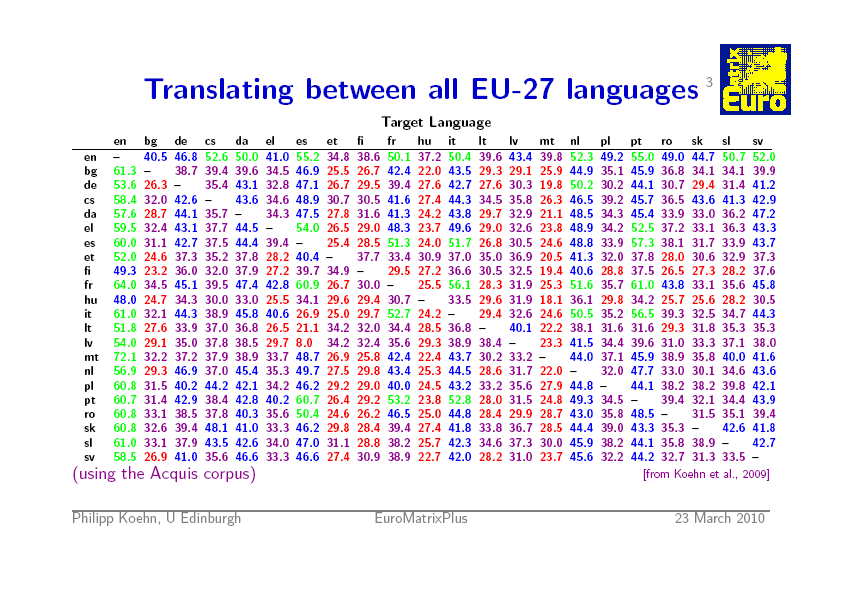
\includegraphics[height=5.0in]{../_media/french/french_table1_mt_matrix.png}
%   \caption{Performances (mesure BLEU) de Traduction Automatique pour un ensemble de paires de langues constitué à partir de 22 langues officielles de l'Union Européenne~\cite{mt462}. La langue source est donnée en ligne et la langue cible est donnée en colonne.}
%   \label{fig:euromatrixplus}
% \end{center}
% \end{figure*}

Cette figure donne la meilleure performance obtenue pour 462 paires de
langues officielles de l'Union Européenne (l'irlandais est manquant),
en termes de score BLEU (plus le score est grand, meilleure est la
traduction~; un traducteur humain obtiendrait environ 80). Les
meilleurs résultats (en vert et bleu) sont pour les langues qui
bénéficient d'un effort de recherche considérable, au sein de
programmes coordonnés, et de l'existence de nombreux corpus parallèles
(anglais, français, néerlandais, espagnol, allemand, etc.), les pires
(en rouge) pour les langues qui ne bénéficient pas d'efforts
semblables, ou qui sont très différentes d'autres langues (hongrois,
maltais, finlandais etc.).

La France est très active dans le domaine de la traduction
automatique, avec des sociétés comme Systran, qui a été un pionnier
dans ce domaine et a fourni la technologie initialement proposée par
Google parmi ses outils linguistiques, avant que Google ne développe
et utilise sa propre technologie, ou Softissimo. Lingua et Machina
propose des mémoires de traduction à des traducteurs
humains. Plusieurs laboratoires mènent également des recherches dans
ce domaine, et obtiennent des résultats qui se situent à l'état de
l'art.\\

\subsubsection{Autre domaines d'application}

Créer des applications à base de technologies de la langue implique
une gamme de sous-tâches qui ne font pas toujours surface au niveau de
l'interaction avec l'utilisateur, mais qui fournissent des
fonctionnalités de service importantes «~sous le capot» du
système. Elles constituent par conséquent des sujets de recherche
importants qui sont devenus des sous-disciplines de la linguistique
computationnelle dans le milieu universitaire.

La {\bf Réponse aux Questions} est devenu un domaine de recherche actif pour
lequel des corpus annotés ont été produits et des compétitions
scientifiques ont été ouvertes. Le principe consiste à passer de la recherche
basée sur des mots-clés (à laquelle le moteur de recherche répond avec
toute une collection de documents potentiellement pertinents) au
scénario d'un utilisateur posant une question concrète et du système
lui fournissant une seule réponse~: 
\begin{itemize}
\item[] \textit{- À quel âge Neil Armstrong a-t-il marché sur la lune~?}
\item[] \textit{- À 38  ans.}
\end{itemize}
Même si ce domaine est évidemment lié au thème global de la recherche
sur le Web susmentionné, la dénomination Réponse aux Questions est
aujourd'hui essentiellement un terme générique qui couvre
différentes problématiques de recherche telles que~: comment
identifier le type d'une question (par ex. question factuelle ou
définitoire) et la traiter en conséquence?, comment synthétiser une
réponse à partir de plusieurs documents pouvant apporter des éléments
d'information contradictoires?, ou comment la réponse peut-elle être
extraite d'un document appartenant à un autre champ thématique que
celui de la question, mais qui contient néanmoins l'information
recherchée?

Cela est également lié à la tâche d'{\bf extraction d'information}
(IE), un domaine qui était extrêmement populaire et influent à
l'époque du «~virage statistique~» en linguistique computationnelle,
au début des années 1990. L'IE vise à identifier des éléments précis
d'information dans des classes spécifiques de documents, par exemple
la détection des principaux acteurs dans les prises de contrôle de
sociétés comme relaté dans les articles de journaux. Un autre scénario
qui a été élaboré concerne les rapports sur les incidents terroristes,
où le problème est de mettre en correspondance le texte avec un
formulaire spécifiant l'auteur, la cible, l'heure et le lieu et les
résultats de l'incident. Le remplissage d'un formulaire spécifique à
un domaine est la caractéristique centrale de l'IE, qui pour cette
raison, est un autre exemple de technologie «~en coulisses~» qui
constitue un domaine de recherche bien délimité, mais qui pour des
raisons pratiques, doit ensuite être intégrée dans un environnement
d'application approprié. Dans certains domaines, comme la veille technologique ou
l'analyse de sentiments ou la fouille d'opinions, ils sont même devenus des modules clé des
architectures standard des applications.

Il existe des domaines en technologies des langues qui concernent à la fois des applications autonomes et des fonctions de base des systèmes de traitement d'information, comme par exemple~: {\bf le résumé automatique de texte} et {\bf la génération de texte}. Résumer se réfère à la tâche de
rendre court un texte long, et est offert, par exemple comme une
fonctionnalité dans MS~Word. Cela fonctionne essentiellement sur une
base statistique, en identifiant d'abord les mots
«~importants~» dans le texte (par exemple, les mots qui sont très
fréquents dans le texte, mais nettement moins fréquents dans l'usage général de la langue) et en déterminant ensuite les phrases
qui contiennent de nombreux mots «~importants~». Ces phrases sont
ensuite marquées dans le document, ou extraites, et sont retenues pour
constituer le résumé. Dans ce scénario, qui est de loin le plus
populaire, résumer revient donc à extraire des phrases : le texte est
réduit à un sous-ensemble de ses phrases. Tous les résumeurs
commerciaux sont fondés sur ce principe. Une approche alternative, à laquelle
sont consacrées quelques recherches, est de générer de nouvelles
phrases, c'est-à-dire, de construire des phrases de résumé qui
n'apparaissent pas sous cette forme dans le texte source. Cela
nécessite un niveau de compréhension plus profond du texte et est donc
beaucoup moins robuste. Un générateur de texte n'est, dans la
plupart des cas, pas une application isolée, mais intégrée dans un
environnement plus large de logiciels, tels que dans un système
d'information hospitalier, où les données du patient sont
collectées, stockées et traitées, et où la génération de rapport
n'est juste qu'une des nombreuses fonctionnalités
offertes.

Pour le français, la situation dans tous ces domaines de recherche est
beaucoup moins développée que pour l'anglais, où la Réponse aux
Questions, l'extraction d'information, et le résumé automatique ont
fait l'objet depuis les années 1990 de nombreuses compétitions
ouvertes, principalement celles qui sont organisées par la DARPA et le
NIST aux États-Unis. Celles-ci ont permis d'améliorer considérablement
l'état de l'art, mais l'accent a le plus souvent été placé sur
l'anglais ou sur des langues d'importance géopolitique pour les
États-Unis. Certaines compétitions ont ajouté des pistes multilingues
ou interlingues, comme les campagnes d'évaluation menées dans le
projet CLEF (Cross-Language Evaluation Forum)~\cite{clef} de la
Commission Européenne, mais le français n'a jamais été prééminent. En
conséquence, il n'y a guère de corpus annotés ou d'autres ressources
pour la plupart de ces tâches. Les systèmes de résumé automatique,
lorsqu'ils utilisent des méthodes purement statistiques, sont souvent
dans une bonne mesure indépendants de la langue, et donc quelques
prototypes de recherche sont disponibles.

Concernant la génération de texte, les composants réutilisables ont
traditionnellement été limités à la réalisation de modules de
réalisation de surface (les «~grammaires de génération~»); là encore,
la plupart des logiciels disponibles le sont pour l'anglais.

\subsubsection{Traitement automatique de la Langue des Signes}

Le Traitement automatique de la Langue des Signes est un domaine de
recherche en pleine expansion, qui va avec le développement de
l'utilisation de la Langue des Signes par les personnes sourdes, et
avec l'obligation légale de fournir un accès à l'information pour les
personnes handicapées. La {\em Langue des Signes Française} (LSF) ne
doit pas être considérée comme une variante de la langue française,
mais comme une langue en soi. Nous mentionnerons donc seulement que
son traitement comporte l'analyse (basée sur le traitement d'image, et
nécessitant la reconnaissance des gestes, des expressions faciales et
des postures), la production (sous la forme d'agents conversationnels)
et même la traduction d'une Langue des Signes à l'autre. Plusieurs
laboratoires travaillent en France sur ce sujet de recherche, et les
premiers résultats ont permis notamment d'équiper certaines gares en France avec
des informations en langue des signes pour les sourds.

\subsection{L'effort technologique sur le français}

\subsubsection{Études sur les Technologies de la Langue pour le français}

Plusieurs études du domaine des technologies de la langue ont été
menées en France, tels que le rapport DGLFLF sur les défis culturels
des technologies de la langue en 2007~\cite{dglflf07}, le rapport du
Forum des droits de l'Internet «~Développement durable et
  Internet~: langues et Internet~» en 2009~\cite{droitsinternet07},
l'étude de marché sur les technologies de la langue en Europe
réalisée pour le Ministère de la Recherche par le Bureau Van Dijk en
2007~\cite{vandijk07} ou le Livre Blanc de l'APIL sur les
industries de la langue en 2005~\cite{apil05}. Le ministère français
de la Culture et de la Communication a produit en 2011 une étude sur
les usages et les applications des technologies de la langue pour le
français, avec un intérêt particulier pour les dimensions culturelles
et économiques.

\subsubsection{Financements}

Les financements de la recherche et développement en technologies de
la langue viennent principalement du Ministère de l'Enseignement
Supérieur et de la Recherche à travers l'Agence Nationale de la
Recherche (ANR), du Ministère de l'Économie, des Finances et de
l'Industrie à travers l'Agence OSEO et à travers les Pôles de
Compétitivité, qui rassemblent industriels et chercheurs, et sont
financés par plusieurs ministères et administrations locales
(départements et régions). La Direction Générale de l'Armement du
Ministère de la Défense a ses propres programmes pour les applications
de défense, et collabore également avec les organismes déjà mentionnés
sur des programmes de coopération concernant les technologies duales
(civil et défense), comme le sont les technologies de la langue.

\subsubsection{Programmes}

Les recherches sur la langue française ont été soutenues par plusieurs
programmes. Le Réseau francophone d'Ingénierie de la Langue
(FRANCIL) a été soutenu par l'Association des Universités
Francophones (AUF, anciennement AUPELF) de 1994 à 2000. Il incluait
des projets de coopération entre les pays francophones du Nord et ceux
du Sud (en particulier en Afrique et en Asie) et des projets de
«~coopétition~» (mélange de coopération et de compétition) organisés comme
des campagnes d'évaluation de technologies à la fois pour le
traitement du langage écrit et du langage parlé.

Le programme TechnoLangue (2003-2005)~\cite{technolangue} a été
soutenu par les Ministères de la Recherche, de l'Industrie et
de la Culture, suite à un rapport du Conseil Supérieur de la Langue
Française. Il comprenait le développement de ressources linguistiques
(corpus, lexiques, dictionnaires, etc.) pour le français et l'organisation de huit campagnes d'évaluation sur des sujets
tels que l'analyse syntaxique, la traduction automatique, la
recherche d'information (Réponse aux Questions) ou la
transcription d'émissions radiodiffusées (campagne
ESTER). Toutes les données et outils produits au sein de ces campagnes
d'évaluation ont été distribués sous forme de boîtes à outils
d'évaluation. Ce programme a été suivi sur la même base par le
programme TechnoVision concernant la recherche en Vision par
Ordinateur, comprenant la reconnaissance optique de caractères (OCR)
et le traitement des documents (y compris la reconnaissance de l'écriture manuscrite). Certaines de ces activités sont maintenant
prolongées sous forme de projets indépendants soutenus par l'ANR, qui a par ailleurs organisé le défi REPERE (2010-2013) sur
l'identification multimodale (texte, parole, image) des
personnes.

Le CNRS (Centre National de la Recherche Scientifique) a eu plusieurs
programmes dans ce domaine au fil des ans, soit dans les STIC ou en
SHS (GRECO, CCIIL, Silfide (avec l'AUPELF), le CRN (incluant le CNTRL~\cite{cnrtl}
et le CRDO~\cite{crdo}~\cite{crdo2})), et le Ministère français de la Recherche a mis en
place en 2011 une Infrastructure de Corpus~\cite{infracorpus} dans le domaine des
Sciences Humaines et Sociales, en lien avec le projet CLARIN de la
Commission Européenne.

Ces programmes ont beaucoup aidé à rassembler la communauté
scientifique autour d'un objectif commun et ont permis la production
de données (corpus, lexiques, dictionnaires, etc.), qui sont cruciales
pour le développement des technologies. Grâce à ces efforts, le
français est classé 3\raise+.5ex\hbox{ème} après l'anglais et l'allemand en termes de
nombre de ressources linguistiques pour la traduction automatique
disponibles pour les langues officielles de l'Union Européenne, tel
que cela apparaît dans l'Euromatrix+~\cite{euromatrixplus} (voir figure \ref{fig:EuromatrixRessourceFr}), où 130
ressources ont été identifiées pour le français (en mai 2011).

\begin{figure*}[tbp]
  \centering
  \begin{tabular}{lrrrrrr}
        & anglais  & allemand & français & espagnol & italien & ... \\
    anglais & \cellcolor{corange5}257 & \cellcolor{corange2}111 & \cellcolor{corange2}109 & \cellcolor{corange2}107 & \cellcolor{corange2}100 &  \cellcolor{corange1} \\     
    allemand & \cellcolor{corange2}111 & \cellcolor{corange4}140 &  \cellcolor{corange1}79 &  \cellcolor{corange1}42 & \cellcolor{corange1}38 & \cellcolor{corange1}\\     
    français & \cellcolor{corange2}109 & \cellcolor{corange1}79 & \cellcolor{corange3}130 &  \cellcolor{corange1}66 & \cellcolor{corange1}52 & \cellcolor{corange1}\\     
    espagnol & \cellcolor{corange2}105 & \cellcolor{corange1}40 &  \cellcolor{corange1}65 & \cellcolor{corange2}128 & \cellcolor{corange1}35 & \cellcolor{corange1}\\     
    italien & \cellcolor{corange2}100 & \cellcolor{corange1}38 &  \cellcolor{corange1}52 &  \cellcolor{corange1}36 & \cellcolor{corange2}116 & \cellcolor{corange1}\\     
    ... & \cellcolor{corange1}    & \cellcolor{corange1}    & \cellcolor{corange1}    & \cellcolor{corange1}    & \cellcolor{corange1}    & \cellcolor{corange1}\\
  \end{tabular}
\caption{Nombre de ressources linguistiques existant pour différentes paires de langues dont le français suivant Euromatrix+}
\label{fig:EuromatrixRessourceFr}
\end{figure*}

La campagne ESTER a permis dans TechnoLangue la production, en 2004,
de 1700 heures de parole concernant les nouvelles radiodiffusées en
français, dont 100 heures ont été transcrites~\cite{ester}, ce qui a permis de
développer des systèmes de transcription de nouvelles radiodiffusées
de qualité suffisante et d'ouvrir la faisabilité de systèmes de
transcription et d'indexation automatiques de vidéo en
français. Toutefois, cela doit être comparé au corpus de nouvelles
radiodiffusées produit pour le chinois au sein du programme américain
DARPA GALE, qui comprend 3000 heures de parole, dont 500 ont été
transcrites manuellement~\cite{gale}!

Aujourd'hui, OSEO soutient le très important programme Quaero qui
rassemble une trentaine de partenaires industriels et académiques avec
un budget total de 200 M€ et un montant de financements publics de 99
M€ sur 5 ans (2008-2013). Quaero porte sur le développement d'une
trentaine de technologies pour différents médias (voix, texte,
musique, image, vidéo) pour les besoins de cinq applications liées au
traitement des documents multimédias et multilingues (plate-forme de
numérisation, analyse de l'impact des médias sociaux, vidéo
personnalisée, portails de communication et patrimoine numérique, et
moteurs de recherche multimédia). Bien que le programme traite
essentiellement de la langue française, certaines technologies seront
développées pour la plupart des 23 langues officielles de
l'UE. L'ensemble du programme est structuré autour de l'évaluation
comparative systématique des technologies et sur la production et
l'utilisation de grandes quantités de données pour l'apprentissage et
l'évaluation des systèmes. En octobre 2011, après 3 années de
fonctionnement du programme, 3 nouvelles applications ont été
ajoutées, incluant de nouveaux partenaires, 45 modules technologiques
ont été livrés et près de 500 articles ont été publiés. L'application
en ligne Voxalead News développée par Exalead en coopération avec le
LIMSI-CNRS, Vocapia Research et l'INRIA, est un excellent exemple des
avancées technologiques rendues possibles dans le cadre de Quaero, en
mettant ensemble des savoir-faire dans 3 domaines différents (moteurs
de recherche, traitement de la parole et traitement de
l'image). Exalead a été acheté par le groupe Dassault Systèmes en 2010.

La France a consacré depuis les années cinquante des efforts
importants pour numériser des textes issus de ses immenses ressources
littéraires. La Bibliothèque National de France (BNF) a lancé un large
effort de numérisation de son fonds patrimonial de documents
nationaux. Ce domaine peut grandement bénéficier des Technologies de
la Langue, qui facilitent l'accès (à l'aide de l'analyse sémantique,
étymologique ou quantitative) aux ressources historiques d'un pays ou
d'une langue. Cela a été bien démontré en 2011 par Google à l'aide de
son corpus Google Books de plus de 500 milliards de mots.

Il n'y a pas de programme comparable dans la partie francophone de la
Belgique, où les sources de financement sont l'Institut pour
l'Encouragement de la Recherche Scientifique et de l'Innovation de
Bruxelles, le Service Public de Wallonie, ou le Fonds National de la
Recherche Scientifique (FNRS). Le Service de la Langue de la
Communauté Française de Belgique a financé le développement de
recherches en terminologie dans le passé et est officiellement en
charge de la coordination des activités terminologiques (au niveau
gouvernemental) dans la partie francophone de la Belgique. L'OWIL
(Observatoire du Traitement Informatique des Langues et de
l'Inforoute) a centralisé d'information sur les activités de recherche
en TAL depuis plusieurs années, mais a cessé ses activités en 2008.

Il n'existe actuellement aucun programme majeur sur les Technologies
de la Langue en Suisse. Le projet le plus pertinent pourrait être le
Centre National de Compétence en Recherche sur la Gestion de
l'Information Interactive Multimodale (IM2), dirigé par l'IDIAP, où
des corpus de parole ont été recueillis, principalement en
collaboration avec les projets AMI et Amida de la Commission Européenne. Il existait un
«~observatoire pour la recherche~», mais le site est maintenant
inactif. Les projets dans tous les domaines, y compris les
technologies de la langue, sont financés par le programme national de
recherche FNSNF.

Le Canada a une agence spéciale pour les Technologies de la Langue :
le CRTL (Centre de Recherche en Technologies Langagières / LTRC -
Language Technology Research Center)~\cite{canadacrtl}. Il y a au
Canada plusieurs équipes universitaires travaillant sur les
technologies de la langue, mais sans qu'il n'y ait de
programme national spécifique, en dehors de programmes nationaux
génériques de recherche.

\subsubsection{Sociétés savantes}

Lorsque l'European Language Resources Association (ELRA)~\cite{elra} a été créée
en 1995, le gouvernement français a exprimé son soutien pour
accueillir son Agence de Distribution des Ressources Linguistiques et
d'Évaluation (ELDA), qui est située à Paris.

La communauté scientifique française et francophone en TAL se réunit
au sein de l'association ATALA qui a récemment célébré son
50\raise+.5ex\hbox{ème} anniversaire et organise la conférence
annuelle TALN, tandis que la communauté francophone en communication
parlée se réunit au sein de l'association AFCP qui organise la
conférence biennale JEP (Journées d'Étude sur la Parole), en
alternance avec la conférence Interspeech lorsqu'elle se situe en
Europe, et en étroite collaboration avec l'International Speech
Communication Association (ISCA), où il constitue un groupe d'intérêt
spécial (SIG). Les conférences TALN et JEP sont organisées
conjointement de temps en temps, et la conférence annuelle RECITAL est
spécialement consacrée aux jeunes chercheurs. L'ATALA maintient la
liste de diffusion LN et, pour les activités des jeunes chercheurs, la
liste de diffusion Orbital, ainsi que le LN-Forum.

Les associations professionnelles, telles que l'APIL (Association des
Professionnels des Industries de la Langue) ou l'association Tenor sur
la parole, ont été très actives dans le passé, mais semblent être
actuellement un peu en sommeil.

L'OEP (Observatoire Européen du Plurilinguisme) est installé en France~\cite{OEP}.

Le Canada a une association industrielle sur les technologies de la langue: AILIA
(Association de l'Industrie de la Langue / {\em Language Industry
Association})~\cite{ailia}.

\subsubsection{Enseignement}
Bien que plus de 30 Universités ou Grandes Écoles d'Ingénieurs
offrent des cours liés aux Technologies de la Langue, soit au sein de
filières de linguistique appliquée ou d'informatique, il
n'existe pas de programmes portant spécifiquement sur la gamme
complète des technologies de langue, y compris les dimensions
technologiques et linguistiques, et couvrant langue parlée, écrite et
signée. La formation des traducteurs et interprètes manque également
d'ouverture suffisante sur les Technologies de la Langue, tel que cela
est apparu lors de la conférence Tralogy'2011~\cite{tralogy},
portant sur la relation entre traducteurs humains et technologies de
la langue.

\subsubsection{Recherche}

En France, il y a environ 50 laboratoires travaillant sur le traitement
automatique de la parole et du langage, ainsi que sur le traitement de
la langue des signes et la communication multimodale, qui
rassemblent environ 600 chercheurs. Beaucoup d'entre eux sont affiliés
à un organisme de recherche de grande taille (CNRS, INRIA (Institut
National pour la Recherche en Informatique et Automatique), CEA
(énergie atomique) et Institut Télécom, qui sont partenaires de
l'Alliance nationale Allistene) ou à des universités et Grandes Écoles.

Certains laboratoires ont obtenu des performances au meilleur niveau
dans le cadre des campagnes d'évaluation internationales, telles que
celles organisées sur la reconnaissance vocale par le NIST aux
Etats-Unis, ou sur les Réponses aux Questions dans le projet CLEF en
Europe.

Des instituts publics participent également à ce domaine de
recherche, tels que le Laboratoire National de Métrologie et d'Essais
(LNE), qui développe des activités liées à l'évaluation des
technologies de la langue, l'INA (Institut National de l'Audiovisuel)
ou la BNF (Bibliothèque Nationale de France), concernant le traitement
de leur énorme quantité de données textuelles ou audiovisuelles.

Plusieurs laboratoires mènent également des recherches sur les
technologies de la langue appliquées à la langue française en Belgique
(Université Libre de Bruxelles, Université de Mons, Université
Catholique de Louvain, etc.), Suisse (IDIAP, EPFL, Université de
Genève, etc.) et le Canada (Université de Montréal, École
Polytechnique de Montréal, CRIM, Université du Québec à Chicoutimi,
etc.).

\subsubsection{Industrie}

Comme mentionné dans le rapport Euromap en 2003~\cite{euromap}, «{\textit{La
France est un acteur majeur en matière de technologies de la langue
dans l'UE, avec une longue tradition de recherche, des laboratoires de
classe mondiale et la couverture de tous les principaux domaines
d'activités. Elle a aussi nourri une communauté respectable de
fournisseurs commerciaux, certains à l'échelle européenne et
mondiale. La recherche a bénéficié d'un soutien conséquent du secteur
public, et la France a été un acteur clé dans l'UE des projets de
recherche collaboratifs.}}»

Les grandes sociétés ont été actives dans ce domaine il y a quelques
années (Alcatel, Thomson, France Télécom (FT)), mais ont diminué leur
effort de recherche, créant parfois des sociétés essaimées ({\em
  spin-off}), comme FT avec Telisma en reconnaissance vocale, ensuite
rachetée par la société indienne OnMobile Global Ltd. Plusieurs PME ou
TPE sont très actives dans les technologies de la langue et de la
parole, comme Vecsys (qui a récemment été achetée par Bertin
Technologies), Vocapia Research, Sinequa, Synapse Développement,
Syllabs, Tagmatica, Arisem, Bertin, Lingway, Pertimm, Systran,
Softissimo, A2iA, VisionObject, etc., tandis que d'autres
sociétés de grande taille (Technicolor, Orange, Exalead (qui fait
maintenant partie de Dassault Systèmes), EADS / Cassidian, Bertin,
etc.) ou de plus petite taille (Temis, Jouve, Aldebaran, Parrot, etc.)
développent des activités en étroite relation avec les fournisseurs de
technologies de la langue. XEROX dispose d'une offre multilingue en
technologies des langues et possède un centre de recherche européen à
Grenoble. Il y a aussi des PME très actives en Belgique (Acapela) ou
au Canada (Nüecho).

L'étude sur la taille de l'industrie de la langue dans l'Union
Européenne, commanditée par la Commission Européenne (DGT) en
2009~\cite{DGT09}, mentionne que 109 entreprises peuvent être
identifiées en France dans le périmètre de l'ingénierie linguistique,
avec un chiffre d'affaires estimé à 78,8 M€, ce qui représente 16\% du
marché européen et place la France comme le deuxième pays en
Europe après le Royaume-Uni.

\subsection{Disponibilité des technologies et des ressources pour le français}



\subsubsection{Tableaux de situation}
Les tableaux suivants (figures \ref{fig:lrlttable_fr_1},
\ref{fig:lrlttable_fr_2}, \ref{fig:lrlttable_fr_3}) donnent un aperçu
de la situation actuelle du soutien technologique pour le français. La
cote des technologies existantes et des ressources est basée sur des
estimations en utilisant les critères suivants (chacun allant de 0 à
6).

\begin{figure*}[!ht]
  \centering
\begin{tabular}{>{\columncolor{orange1}}p{.50\linewidth}@{\hspace*{6mm}}c@{\hspace*{6mm}}c@{\hspace*{6mm}}c@{\hspace*{6mm}}c@{\hspace*{6mm}}c@{\hspace*{6mm}}c@{\hspace*{6mm}}c}
  \rowcolor{orange1}
   \cellcolor{white}
  &\begin{sideways}\makecell[l]{Quantité}\end{sideways}
 % &\begin{sideways}\makecell[l]{\makecell[l]{Disponibilité} }\end{sideways} 
  &\begin{sideways}\makecell[l]{Disponibilité~~~~}\end{sideways}
  &\begin{sideways}\makecell[l]{Qualité}\end{sideways}
  &\begin{sideways}\makecell[l]{Couverture}\end{sideways} 
  &\begin{sideways}\makecell[l]{Maturité}\end{sideways} 
  &\begin{sideways}\makecell[l]{Pérennité}\end{sideways} 
  &\begin{sideways}\makecell[l]{Adaptabilité}\end{sideways} \\ \addlinespace
  \multicolumn{8}{>{\columncolor{orange2}}l}{Technologies de la langue} \\\addlinespace
  Tokenisation, analyse~morpho-syntaxique, analyse/génération morphologique &4&4&4&4&4&3&3 \\ \addlinespace
  Analyse syntaxique (de surface ou profonde) &4&4&4&4&4&2&2\\ \addlinespace
  Sémantique des phrases (WSD, structure argumentaire, rôles sémantiques) &2&2&2&1&2&1&2\\ \addlinespace
  Sémantique de textes (résolution de coréférences, contexte, pragmatique, inférence) &2&1&3&2&2&2&1\\ \addlinespace
  Traitement avancé du discours (structure des textes, cohérence, structure rhétorique/RST, zonage argumentatif, argumentation, patterns textuels, types de textes etc.) &2&2&2&2&2&2&1\\ \addlinespace
  Recherche d'Informations (Indexation de textes, RI multimédia, RI interlingue) &4&5&5&4&5&4&4\\ \addlinespace
  Extraction d'Informations (reconnaissance d'entités nommées, extraction d'évènements/de relations, reconnaissance d'opinions/de sentiments, fouille de textes/analytique)&3&3&4&3&4&3&3\\ \addlinespace
  Génération de Langue (génération de phrases, génération de rapports, génération de textes) &2&1&2&2&2&1&2\\ \addlinespace
  Résumé automatique, Réponse aux Questions, Technologies avancées d'accès à l'Information &3&3&3&3&3&2&2\\ \addlinespace
  Traduction Automatique (et traduction vocale) &5&4&4&3&4&3&3\\ \addlinespace
  Reconnaissance de la parole (couvrant un large spectre: commande vocale, dictée vocale, transcription d'émissions, transcription de conversations, dialogue oral) &4&3&4&4&4&3&3\\ \addlinespace
  Synthèse vocale (synthèse à partir du texte, génération de parole)&4&3&4&4&4&3&3\\ \addlinespace
  Gestion du Dialogue (Capacités dialogiques et modélisation de l'interlocuteur)&3&2&3&3&3&2&2\\ \addlinespace
  \end{tabular}
  \caption{Tableau complet de la situation estimée des technologies du langage pour le français.}
  \label{fig:lrlttable_fr_1}
\end{figure*}


\begin{figure*}[ht]
  \centering
\begin{tabular}{>{\columncolor{orange1}}p{.50\linewidth}@{\hspace*{6mm}}c@{\hspace*{6mm}}c@{\hspace*{6mm}}c@{\hspace*{6mm}}c@{\hspace*{6mm}}c@{\hspace*{6mm}}c@{\hspace*{6mm}}c}
  \rowcolor{orange1}
   \cellcolor{white}
  &\begin{sideways}\makecell[l]{Quantité}\end{sideways}
 % &\begin{sideways}\makecell[l]{\makecell[l]{Disponibilité} }\end{sideways} 
  &\begin{sideways}\makecell[l]{Disponibilité~~~~}\end{sideways}
  &\begin{sideways}\makecell[l]{Qualité}\end{sideways}
  &\begin{sideways}\makecell[l]{Couverture}\end{sideways} 
  &\begin{sideways}\makecell[l]{Maturité}\end{sideways} 
  &\begin{sideways}\makecell[l]{Pérennité}\end{sideways} 
  &\begin{sideways}\makecell[l]{Adaptabilité}\end{sideways} \\ \addlinespace
  \multicolumn{8}{>{\columncolor{orange2}}l}{Ressources Linguistiques} \\\addlinespace
  Corpus de référence &3&1&4&3&4&4&3\\ \addlinespace
  Corpus syntaxiques (corpus arborés)&4&4&3&3&3&3&2\\ \addlinespace
  Corpus sémantiques&2&2&2&1&2&2&2\\ \addlinespace
  Corpus de discours&1&2&2&2&1&1&1\\ \addlinespace
  Corpus parallèles, Mémoires de traduction&4&3&4&3&3&4&2\\ \addlinespace
  Corpus de parole (brut, étiqueté/annoté, dialogue)&4&3&4&3&3&4&2\\ \addlinespace
  Corpus multimédia et multimodal (texte combiné à de l'audio/de la vidéo)&2&1&3&1&1&2&1\\ \addlinespace
  Modèles de langage&4&3&3&3&3&3&2\\ \addlinespace
  Lexiques, Bases terminologiques&4&3&4&3&4&4&3\\ \addlinespace
  Grammaires&3&2&3&3&3&2&2\\ \addlinespace
  Thesauri, WordNets&3&3&2&1&3&3&3\\ \addlinespace
  Ressources Ontologiques pour la connaissance du monde (c.àd. {\em upper models}, Données liées)  &2&1&2&1&2&1&1\\ \addlinespace
  \end{tabular}
  \caption{Tableau complet de la situation estimée des ressources linguistiques pour le français.}
  \label{fig:lrlttable_fr_2}
\end{figure*}


\begin{enumerate}
\item {\bf Quantité}~: Est-ce qu'un outil/une ressource existe pour la langue considérée~? Plus il y en a, meilleure est la note.
      \begin{itemize}
      \item 0~: pas d'outils/ressources quels qu'ils soient  
      \item 6~: de nombreux outils/ressources, d'une grande variété 
      \end{itemize}

\item {\bf Disponibilité}~: Est-ce que les outils/ressources sont accessibles~? Sont-ils Open Source, librement utilisables sur n'importe quelle plateforme ou seulement disponibles pour un prix élevé ou dans des conditions très restreintes~?
      \begin{itemize}
      \item 0~: pratiquement tous les outils/ressources sont disponibles à un prix élevé
      \item 6~: une grande quantité d'outils/ressources sont librement et ouvertement disponibles sous Open Source ou avec des licences Creative Commons qui permettent leur réutilisation
      \end{itemize}

\item {\bf Qualité}~: Quelles sont les performances obtenues par les meilleurs outils disponibles, quelle est la qualité des meilleures ressources~? S'agit-il d'outils / de ressources toujours maintenues~? 
      \begin{itemize}
      \item 0~: ressource/outil jouet
      \item 6~: outil de haute qualité, annotations humaines de haute qualité d'une ressource 
      \end{itemize}

\item {\bf Couverture}~: À quel degré les meilleurs outils répondent-ils aux critères de couverture respectifs (styles, genres, sortes de texte, phénomènes linguistiques, types d'entrées / sorties, nombres de langues prises en charge par un système de traduction automatique, etc.)~? À quel degré les ressources sont-elles représentatives de la langue cible ou de sous-langages~? 
      \begin{itemize}
      \item 0~: Services spécialisés de ressources ou d'outils, cas particuliers, couverture très faible, seulement utilisable pour des cas très spécifiques sans utilisation générale
      \item 6~: ressources avec une très large couverture, outil très robuste, largement applicable, nombreuses langues traitées.
      \end{itemize}

\item {\bf Maturité}~: L'outil/ressource peut-il être considéré comme mature, stable, prêt pour le marché~? Les meilleurs outils / ressources disponibles sont-ils «~prêts à l'emploi~» ou doivent-ils être adaptés~? Est-ce que la performance d'une technologie est adéquate et prête pour une utilisation en production ou est-ce seulement un prototype qui ne peut pas être utilisé pour des systèmes de production~? Un indicateur peut être de savoir si les ressources / outils sont acceptés par la communauté et utilisés avec succès dans des systèmes utilisant les technologies de la langue.  
     \begin{itemize}
      \item 0~: prototype préliminaire, système-jouet, preuve de concept, extraits de ressource
      \item 6~: composant immédiatement intégrable / applicable
      \end{itemize}

\item {\bf Pérennité}~: Comment l'outil / la ressource peut-il être maintenu / intégré dans les systèmes informatiques actuels~? L'outil / la ressource remplit-il un certain niveau de pérennité en matière de documentation / manuel, explication des cas d'utilisation, front-ends, interface utilisateur graphique, etc.~? Utilise-t-il / emploie-t-il des environnements de programmation standards / des bonnes pratiques~? Est-ce qu'il existe des normes / des quasi-standards industriels / de recherche et si oui, l'outil / ressource est-il en conformité (formats de données, etc.)~? 
      \begin{itemize}
      \item 0~: format totalement propriétaire, format de données et API ad hoc
      \item 6~: en plein accord avec les normes de conformité, entièrement documenté
      \end{itemize}

\item {\bf Adaptabilité} : Comment les meilleurs outils / ressources peuvent-ils être adaptés / étendus à de nouvelles tâches / domaines / genres / types de textes / cas d'utilisation etc.~? 
\begin{itemize}
      \item 0~: pratiquement impossible d'adapter un outil / une ressource à une autre tâche, impossible même avec de grandes quantités de ressources ou de personne-mois disponibles
      \item 6~: très haut niveau d'adaptabilité, adaptation envisageable et facilement réalisable.
      \end{itemize}
\end{enumerate}


Un tableau réduit (figure \ref{fig:lrlttable_fr_3}) a également été produit, où les technologies et les
ressources ont été regroupées, qui prend également en compte la comparaison avec les autres langues européennes.

\begin{figure*}[th]
  \centering
\begin{tabular}{>{\columncolor{orange1}}p{.50\linewidth}@{\hspace*{6mm}}c@{\hspace*{6mm}}c@{\hspace*{6mm}}c@{\hspace*{6mm}}c@{\hspace*{6mm}}c@{\hspace*{6mm}}c@{\hspace*{6mm}}c}
  \rowcolor{orange1}
   \cellcolor{white}
  &\begin{sideways}\makecell[l]{Quantité}\end{sideways}
 % &\begin{sideways}\makecell[l]{\makecell[l]{Disponibilité} }\end{sideways} 
  &\begin{sideways}\makecell[l]{Disponibilité~~~~}\end{sideways}
  &\begin{sideways}\makecell[l]{Qualité}\end{sideways}
  &\begin{sideways}\makecell[l]{Couverture}\end{sideways} 
  &\begin{sideways}\makecell[l]{Maturité}\end{sideways} 
  &\begin{sideways}\makecell[l]{Pérennité}\end{sideways} 
  &\begin{sideways}\makecell[l]{Adaptabilité}\end{sideways} \\ \addlinespace
  \multicolumn{8}{>{\columncolor{orange2}}l}{Technologies de la langue} \\\addlinespace
  {\bf Reconnaissance de la parole} &4&3&4&4&4&3&3\\ \addlinespace
  {\bf Synthèse vocale}  &4&3&4&4&4&3&3\\ \addlinespace
  {\bf Analyse grammaticale}  &4&4&4&4&4&3&3\\ \addlinespace
  {\bf Analyse sémantique}  &3&3&3&3&3&2&2\\ \addlinespace
  {\bf Génération de texte} &3&2&3&3&3&2&2\\ \addlinespace
  {\bf Traduction Automatique} &5&4&4&4&4&3&3\\ \addlinespace
  \multicolumn{8}{>{\columncolor{orange2}}l}{Ressources linguistiques} \\\addlinespace
  {\bf Corpus de textes} &4&3&4&4&4&4&3\\ \addlinespace
  {\bf Corpus de parole} &4&3&4&4&4&4&3\\ \addlinespace
  {\bf Corpus parallèles, Mémoires de traduction}&4&3&4&4&4&4&3\\ \addlinespace
  {\bf Ressources lexicales}  &4&3&4&4&4&4&3\\ \addlinespace
  {\bf Grammaires, Modèles de langage}&3&3&4&4&3&3&3\\ \addlinespace
  \end{tabular}
  \caption{Tableau réduit de la situation estimée des technologies du langage et des ressources linguistiques pour le français.} 
%\caption{Tableau réduit de la situation estimée des outils et ressources pour le français (voir~\cite{terminology_table} pour l'explicitation de certains termes.)}
  \label{fig:lrlttable_fr_3}
\end{figure*}

\subsubsection{Interprétation des Tableaux}
Ces tableaux (figures \ref{fig:lrlttable_fr_1}, \ref{fig:lrlttable_fr_2} et \ref{fig:lrlttable_fr_3}) sur l'état des technologies et des
ressources (données, outils, évaluation et méta-ressources) pour la
langue française sont proches de ce qui a été produit pour la langue
allemande. La situation est très similaire, comme cela apparaît dans
les matrices de langue META-Matrixes, et dans les tables bilingues du
projet Euromatrix+~\cite{euromatrixplustableau}. Dans les
META-Matrixes, produites à partir des données obtenues dans la
LRE-Map~\cite{lremap}, il apparaît que, parmi les 23 langues
européennes officielles, le français et l'allemand bénéficient
globalement d'un nombre voisin de ressources (respectivement 143 et
132), loin de ce qui existe pour l'anglais (559), et suivis par
l'espagnol (111) et l'italien (90). Dans la matrice Euromatrix+, produite à
partir du Hutchins Compendium of Translation
Software~\cite{compendiummt}, le français et l'allemand sont également
proches (130 et 140 respectivement), loin de l'anglais (257), et suivis
par l'espagnol (128) et l'italien (116).

\begin{itemize}
\item D'importants programmes ont été menés sur le traitement
  de la langue française, soit dans des programmes français
  (TechnoLangue (2003-2005) soutenu par les ministères de la
  Recherche, de l'Industrie et de la Culture), ou des
  programmes francophones (FRANCIL (1994-2000) soutenu par l'Association des Universités Francophones (AUF)). Ces programmes
  contenaient une grande partie consacrée à la production de
  ressources pour la langue parlée et écrite et à l'évaluation
  des systèmes de traitement du langage parlé et écrit. Cela a permis
  d'assurer la disponibilité de données, d'outils
  évalués, de boîtes à outils d'évaluation et de
  méta-ressources (métadonnées, normes, etc.) pour le français,
  beaucoup d'entre eux étant distribués par ELRA. L'évaluation de plusieurs systèmes sur les mêmes données a permis
  la production de grandes quantités de corpus annotés
  semi-automatiquement (étiqueteurs morpho-syntaxiques dans GRACE,
  analyseurs syntaxiques dans PASSAGE).

\item Dans la mesure où ELDA, l'agence de distribution d'ELRA, est située en
France, de nombreuses ressources linguistiques en français sont
distribuées par ELRA.

\item Le grand programme Quaero (200 M€ de budget sur 5 ans (2008-2013))
soutient un effort important sur le traitement des documents
multimédias et multilingues, y compris le développement des
principales technologies de traitement du langage parlé et écrit, pour
le français et pour d'autres langues (comme la transcription de
parole, la traduction écrite et vocale, les systèmes de réponses aux
questions, l'indexation et la recherche dans les données
audiovisuelles), avec l'objectif de couvrir toutes les langues
officielles de l'UE. Toutes les technologies développées sont
régulièrement évaluées afin de vérifier l'adéquation de leurs
performances avec les besoins des applications ciblées, et un projet
est spécifiquement chargé de la production de corpus pour le
développement et le test des systèmes, avec un budget de 10 M€.

\item La société Exalead du groupe Dassault Systèmes est très active dans le
domaine de la recherche d'informations et des moteurs de recherche. Sa
participation à Quaero a permis à Exalead de développer des
applications innovantes dans le domaine de la recherche audiovisuelle
(Voxalead News) basée sur des technologies avancées de traitement de
la parole et de l'image.

\item La langue française n'a pas de «~corpus national~», un mélange équilibré
de différents genres de textes, comme cela existe en Grande-Bretagne,
aux États-Unis, en Allemagne, en Russie, en Pologne ou en Slovaquie,
tel qu'il apparaît sur le site Web Corpus Based Language Studies~\cite{corpuslangstud},
mais beaucoup de corpus du français existent en France et
ailleurs~\cite{corpusfr}. En outre, un corpus de 260.000.000 mots lemmatisés et
étiquetés morpho-syntaxiquement, extrait du Wikipédia en français, est
disponible~\cite{wikipediafr}. Le corpus Frantext de l'ATILF~\cite{atilf} a été mis à disposition
depuis de nombreuses années, incluant la plupart des textes de la
littérature du 20ème siècle, et des corpus plus récents de normes
techniques AFNOR, de français contemporain et de variantes régionales
du français.

\item Il n'y a pas de grand corpus arboré ({\em Treebank}) pour le français. Le projet ANR PASSAGE
devrait produire très prochainement un important corpus étiquetés
syntaxiquement pour le français, non sous la forme d'arbres
syntaxiques, mais de relations grammaticales.

\item Les corpus parallèles bilingues pour le français bénéficient de
sources européennes, telles que les traductions dans les organes de
l'UE (Commission Européenne, Parlement Européen, Cour de Justice
Européenne, Office Européen des Brevets, etc.), mais aussi venant de
pays bilingues comme le Canada. Des corpus parallèles existent avec la
plupart des autres langues européennes. Les langues les moins bien représentées
sont le slovaque, l'estonien, le maltais et l'irlandais. Ces
corpus parallèles sont adaptés à des applications dans les domaines
politiques ou administratifs pour la langue écrite, tandis que
d'autres domaines d'application tels que la traduction d'émissions
radio ou télévisées manquent d'une quantité suffisante de données.

\item En lien avec cette disponibilité de corpus parallèles, des systèmes de
Traduction Automatique sont disponibles pour toutes les paires de
langues de l'UE incluant le français. La meilleure qualité de
traduction est réalisée pour les langues source ou cible où une grande
quantité de corpus parallèles existe (anglais) et/ou pour les langues
qui appartiennent à la famille des langues romanes (espagnol, italien,
portugais, roumain). Les résultats les moins bons sont obtenus à partir du et
vers le finlandais, et du français vers l'estonien, le hongrois, le
letton et le maltais.

\item En France, plusieurs entreprises commercialisent depuis de nombreuses
années des systèmes de traduction automatique (Systran (qui était la
technologie initialement utilisée par Google pour son service de
traduction en ligne), Softissimo (Reverso)) ou d'aides aux traducteurs
(Lingua et Machina).

\item De même, la France est très active dans le domaine de la
reconnaissance vocale. Elle maîtrise des technologies qui sont au
meilleur niveau de l'état de l'art, comme cela apparaît dans les
campagnes d'évaluation internationales, et plusieurs PME sont actives
dans ce domaine (comme Vecsys, ou Vocapia Research). Des taux de
reconnaissance proches de 85\% pour la transcription d'émissions de
radio ou de télévision, dans des conditions normales de diffusion,
sont maintenant obtenus par des technologies françaises sur la langue
française, mais aussi sur d'autres langues (anglais, arabe, russe,
chinois mandarin, espagnol), ce qui permet d'effectuer l'indexation automatique
de données audiovisuelles. La recherche d'information interlingue est
également possible en ajoutant de la traduction automatique.

\item La France est également très active dans la reconnaissance du
locuteur, et participe régulièrement avec d'excellents résultats aux
campagnes d'évaluation Odyssey organisées par le NIST.

\item En accord avec cet intérêt pour la reconnaissance vocale, des
ressources ont été disponibles très tôt pour le français parlé (le
corpus BREF en 1990, ou le lexique de prononciation BDLex en 1996, qui
sont distribués par ELRA).

\item Il existe plusieurs WordNet pour le français (EuroWordNet, Wolf
  de l'INRIA, le WordNet du CEA (appelé JAWS)), mais pas aussi
  complets que le WordNet initial de Princeton ou encore que le
  WordNet allemand élargi dans le projet Kyoto de la Commission
  Européenne, où le français n'est pas pris en compte.

\item Il n'y a pas encore de grand FrameNet pour le français, malgré
quelques initiatives en cours basées sur la traduction du FrameNet
américain, alors qu'il existe pour l'allemand. Cependant, il existe
des lexiques grammaticaux et des dictionnaires syntaxiques
(Dicovalence de l'Université catholique de Louvain, Lefff d'INRIA
Alpage, Unitex de l'institut Gaspard-Monge, NooJ de M. Silberztein).

\item Beaucoup de ressources souffrent d'un manque de normalisation,
  et donc, même si elles existent, leur pérennité n'est pas
  assurée; des programmes concertés et des initiatives sont
  nécessaires pour normaliser les données et les formats d'échange. À noter cependant l'émergence ponctuelle de nouvelles
  normes, comme par exemple la norme de représentation des dictionnaires LMF~\cite{LMF}.

\item Traiter la sémantique est plus difficile que traiter la syntaxe ;
traiter la sémantique d'un texte est plus difficile que traiter la
sémantique d'un mot ou d'une phrase, et encore davantage pour la sémantique
du discours. La taille de l'effort pour annoter sémantiquement un
corpus est énorme.

\item Plus un outil a à traiter des questions sémantiques, plus il est
difficile de trouver les données adéquates et de développer des
systèmes portables; et plus grands seront les efforts nécessaires pour
effectuer des traitements en profondeur.

\item Certes, des normes existent pour la sémantique au sens de la
connaissance du monde (RDF, OWL, etc.), mais elles ne sont cependant
pas facilement applicables dans le domaine du TAL.

\item La recherche a réussi à concevoir des logiciels de qualité, mais il
est difficile d'offrir des solutions durables et standardisées compte
tenu des situations actuelles de financement.
\end{itemize}

\subsubsection{Comparaison entre langues}

L'état actuel des Technologies de la Langue varie considérablement
d'une langue à l'autre. Afin de comparer la situation pour les
différentes langues, cette section présente une évaluation faite par
les partenaires de META-NET et basée sur trois technologies (la
traduction automatique, le traitement de la parole et l'analyse de
texte), ainsi que sur les ressources nécessaires pour produire ces
technologies.

Les langues ont été classées en utilisant une échelle sur 5 niveaux~:
\begin{enumerate}
\item Excellente base
\item Bonne base
\item Base moyenne
\item Base fragmentée
\item Base faible ou inexistante
\end{enumerate}

La catégorisation a été faite avec les critères suivants~:\\

{\bf Traitement de la parole}~: Qualité des technologies de
reconnaissance de la parole existantes, qualité des technologies de
synthèse vocale existantes, couverture des domaines, nombre et taille
des corpus de parole existants, nombre et variété des applications à
base de technologies vocales existantes.

{\bf Traduction automatique}~: Qualité des technologies de traduction
automatique existantes, nombre de paires de langues couvertes,
couverture des phénomènes et des domaines linguistiques, qualité et
taille des corpus parallèles existants, nombre et variété des
applications de traduction automatique.

{\bf Analyse de texte}~: Qualité et couverture des technologies
d'analyse de texte existantes (morphologie, syntaxe, sémantique),
couverture des phénomènes et des domaines linguistiques, nombre et
variété des applications, qualité et taille des corpus (annotés)
existants, qualité et couverture des ressources lexicales existantes
(par exemple WordNet) et des grammaires.

{\bf Ressources}~: Qualité et taille des corpus de texte et de parole,
et des corpus parallèles existants, qualité et couverture des
ressources lexicales et des grammaires existantes

\begin{figure*}[h]
  \small
  \centering
  \begin{tabular}
  { 
  >{\columncolor{corange5}}p{.13\linewidth}@{\hspace{.040\linewidth}}
  >{\columncolor{corange4}}p{.13\linewidth}@{\hspace{.040\linewidth}}
  >{\columncolor{corange3}}p{.13\linewidth}@{\hspace{.040\linewidth}}
  >{\columncolor{corange2}}p{.13\linewidth}@{\hspace{.040\linewidth}}
  >{\columncolor{corange1}}p{.13\linewidth} 
  }
  \multicolumn{1}{>{\columncolor{white}}c@{\hspace{.040\linewidth}}}{\textbf{Excellente}} & 
  \multicolumn{1}{@{}>{\columncolor{white}}c@{\hspace{.040\linewidth}}}{\textbf{Bonne}} &
  \multicolumn{1}{@{}>{\columncolor{white}}c@{\hspace{.040\linewidth}}}{\textbf{Base}} &
  \multicolumn{1}{@{}>{\columncolor{white}}c@{\hspace{.040\linewidth}}}{\textbf{Base}} &
  \multicolumn{1}{@{}>{\columncolor{white}}c}{\textbf{Base}} \\ 
  \multicolumn{1}{>{\columncolor{white}}c@{\hspace{.040\linewidth}}}{\textbf{base}} & 
  \multicolumn{1}{@{}>{\columncolor{white}}c@{\hspace{.040\linewidth}}}{\textbf{base}} &
  \multicolumn{1}{@{}>{\columncolor{white}}c@{\hspace{.040\linewidth}}}{\textbf{moyenne}} &
  \multicolumn{1}{@{}>{\columncolor{white}}c@{\hspace{.040\linewidth}}}{\textbf{fragmentée}} &
  \multicolumn{1}{@{}>{\columncolor{white}}c}{\textbf{faible/inexistante}} \\ \addlinespace

  & \vspace*{0.5mm}Anglais 
  & \vspace*{0.5mm}Allemand \newline   
  Espagnol \newline
  Finnois \newline 
  \textbf{Français} \newline
  Italien \newline   
  Néerlandais \newline 
  Portugais \newline 
  Tchèque 
  & \vspace*{0.5mm}Basque \newline 
  Bulgare \newline 
  Catalan \newline 
  Danois \newline 
  Estonien \newline 
  Galicien \newline 
  Grec \newline  
  Hongrois \newline
  Irlandais \newline  
  Novégien \newline 
  Polonais \newline 
  Serbe \newline 
  Slovaque \newline 
  Slovène \newline 
  Suédois 
  & \vspace*{0.5mm}  Croate \newline  
  Islandais\newline 
  Letton \newline 
  Lituanien \newline 
  Maltais \newline 
  Roumain \\
  \end{tabular}
  \caption{Traitement de la parole : état de la technologie pour 30 langues européennes}
  \label{fig:speech_cluster_fr}
\end{figure*}

\begin{figure*}[h]
  \small
  \centering
  \begin{tabular}
  { 
  >{\columncolor{corange5}}p{.13\linewidth}@{\hspace{.040\linewidth}}
  >{\columncolor{corange4}}p{.13\linewidth}@{\hspace{.040\linewidth}}
  >{\columncolor{corange3}}p{.13\linewidth}@{\hspace{.040\linewidth}}
  >{\columncolor{corange2}}p{.13\linewidth}@{\hspace{.040\linewidth}}
  >{\columncolor{corange1}}p{.13\linewidth} 
  }
  \multicolumn{1}{>{\columncolor{white}}c@{\hspace{.040\linewidth}}}{\textbf{Excellente}} & 
  \multicolumn{1}{@{}>{\columncolor{white}}c@{\hspace{.040\linewidth}}}{\textbf{Bonne}} &
  \multicolumn{1}{@{}>{\columncolor{white}}c@{\hspace{.040\linewidth}}}{\textbf{Base}} &
  \multicolumn{1}{@{}>{\columncolor{white}}c@{\hspace{.040\linewidth}}}{\textbf{Base}} &
  \multicolumn{1}{@{}>{\columncolor{white}}c}{\textbf{Base}} \\ 
  \multicolumn{1}{>{\columncolor{white}}c@{\hspace{.040\linewidth}}}{\textbf{base}} & 
  \multicolumn{1}{@{}>{\columncolor{white}}c@{\hspace{.040\linewidth}}}{\textbf{base}} &
  \multicolumn{1}{@{}>{\columncolor{white}}c@{\hspace{.040\linewidth}}}{\textbf{moyenne}} &
  \multicolumn{1}{@{}>{\columncolor{white}}c@{\hspace{.040\linewidth}}}{\textbf{fragmentée}} &
  \multicolumn{1}{@{}>{\columncolor{white}}c}{\textbf{faible/inexistante}} \\ \addlinespace

  & \vspace*{0.5mm}Anglais  
  & \vspace*{0.5mm}Espagnol \newline 
  \textbf{Français}
  & \vspace*{0.5mm}Allemand \newline 
  Catalan \newline 
  Hongrois \newline 
  Italien \newline 
  Néerlandais \newline 
  Polonais \newline 
  Roumain 
  & \vspace*{0.5mm}Basque \newline 
  Bulgare \newline 
  Croate \newline 
  Danois \newline 
  Estonien \newline 
  Finnois \newline 
  Galicien \newline 
  Grec \newline 
  Irlandais \newline 
  Islandais \newline 
  Letton \newline 
  Lituanien \newline 
  Maltais \newline 
  Norvégien \newline 
  Portugais \newline 
  Serbe \newline 
  Slovaque \newline 
  Slovène \newline 
  Suédois \newline 
  Tchèque 
  \end{tabular}
  \caption{Traduction Automatique : état de la technologie pour 30 langues européennes}
  \label{fig:mt_cluster_fr}
\end{figure*}

\begin{figure*}[h]
  \small
  \centering
  \begin{tabular}
  { 
  >{\columncolor{corange5}}p{.13\linewidth}@{\hspace{.040\linewidth}}
  >{\columncolor{corange4}}p{.13\linewidth}@{\hspace{.040\linewidth}}
  >{\columncolor{corange3}}p{.13\linewidth}@{\hspace{.040\linewidth}}
  >{\columncolor{corange2}}p{.13\linewidth}@{\hspace{.040\linewidth}}
  >{\columncolor{corange1}}p{.13\linewidth} 
  }
  \multicolumn{1}{>{\columncolor{white}}c@{\hspace{.040\linewidth}}}{\textbf{Excellente}} & 
  \multicolumn{1}{@{}>{\columncolor{white}}c@{\hspace{.040\linewidth}}}{\textbf{Bonne}} &
  \multicolumn{1}{@{}>{\columncolor{white}}c@{\hspace{.040\linewidth}}}{\textbf{Base}} &
  \multicolumn{1}{@{}>{\columncolor{white}}c@{\hspace{.040\linewidth}}}{\textbf{Base}} &
  \multicolumn{1}{@{}>{\columncolor{white}}c}{\textbf{Base}} \\ 
  \multicolumn{1}{>{\columncolor{white}}c@{\hspace{.040\linewidth}}}{\textbf{base}} & 
  \multicolumn{1}{@{}>{\columncolor{white}}c@{\hspace{.040\linewidth}}}{\textbf{base}} &
  \multicolumn{1}{@{}>{\columncolor{white}}c@{\hspace{.040\linewidth}}}{\textbf{moyenne}} &
  \multicolumn{1}{@{}>{\columncolor{white}}c@{\hspace{.040\linewidth}}}{\textbf{fragmentée}} &
  \multicolumn{1}{@{}>{\columncolor{white}}c}{\textbf{faible/inexistante}} \\ \addlinespace

  & \vspace*{0.5mm}Anglais 
  & \vspace*{0.5mm}Allemand \newline 
  Espagnol \newline 
  \textbf{Français} \newline 
  Italien \newline 
  Néerlandais
  & \vspace*{0.5mm}Basque \newline 
  Bulgare \newline
  Catalan \newline  
  Danois \newline 
  Finnois \newline 
  Galicien \newline 
  Grec \newline 
  Hongrois \newline 
  Norvégien \newline 
  Polonais \newline 
  Portugais \newline 
  Roumain \newline 
  Slovaque \newline 
  Slovène \newline 
  Suédois \newline 
  Tchèque 
  & \vspace*{0.5mm}Croate \newline 
  Estonien \newline 
  Irlandais \newline 
  Islandais \newline 
  Letton \newline 
  Lituanien \newline 
  Maltais \newline 
  Serbe \\
  \end{tabular}
  \caption{Analyse de textes : état de la technologie pour 30 langues européennes}
  \label{fig:text_cluster_fr}
\end{figure*}

\begin{figure*}[h]
  \small
  \centering
  \begin{tabular}
  { 
  >{\columncolor{corange5}}p{.13\linewidth}@{\hspace{.040\linewidth}}
  >{\columncolor{corange4}}p{.13\linewidth}@{\hspace{.040\linewidth}}
  >{\columncolor{corange3}}p{.13\linewidth}@{\hspace{.040\linewidth}}
  >{\columncolor{corange2}}p{.13\linewidth}@{\hspace{.040\linewidth}}
  >{\columncolor{corange1}}p{.13\linewidth} 
  }
  \multicolumn{1}{>{\columncolor{white}}c@{\hspace{.040\linewidth}}}{\textbf{Excellente}} & 
  \multicolumn{1}{@{}>{\columncolor{white}}c@{\hspace{.040\linewidth}}}{\textbf{Bonne}} &
  \multicolumn{1}{@{}>{\columncolor{white}}c@{\hspace{.040\linewidth}}}{\textbf{Base}} &
  \multicolumn{1}{@{}>{\columncolor{white}}c@{\hspace{.040\linewidth}}}{\textbf{Base}} &
  \multicolumn{1}{@{}>{\columncolor{white}}c}{\textbf{Base}} \\ 
  \multicolumn{1}{>{\columncolor{white}}c@{\hspace{.040\linewidth}}}{\textbf{base}} & 
  \multicolumn{1}{@{}>{\columncolor{white}}c@{\hspace{.040\linewidth}}}{\textbf{base}} &
  \multicolumn{1}{@{}>{\columncolor{white}}c@{\hspace{.040\linewidth}}}{\textbf{moyenne}} &
  \multicolumn{1}{@{}>{\columncolor{white}}c@{\hspace{.040\linewidth}}}{\textbf{fragmentée}} &
  \multicolumn{1}{@{}>{\columncolor{white}}c}{\textbf{faible/inexistante}} \\ \addlinespace
  
  & \vspace*{0.5mm}Anglais 
  & \vspace*{0.5mm}Allemand \newline 
    Espagnol \newline
    \textbf{Français} \newline 
    Hongrois \newline
    Italien \newline
    Néerlandais \newline 
    Polonais \newline 
    Suédois \newline 
    Tchèque
  & \vspace*{0.5mm}  Basque \newline 
    Bulgare \newline 
    Catalan \newline 
    Croate \newline 
    Danois \newline 
    Estonien \newline 
    Finnois \newline 
    Galicien \newline 
    Grec \newline 
    Norvégien \newline 
    Portugais \newline 
    Roumain \newline 
    Serbe \newline 
    Slovaque \newline 
    Slovène
  &  \vspace*{0.5mm} Irlandais \newline 
    Islandais \newline 
    Letton \newline 
    Lituanien \newline 
    Maltais \\
  \end{tabular}
  \caption{Ressources linguistiques : état pour 30 langues européennes}
  \label{fig:resources_cluster_fr}
\end{figure*}

Les tables des figures \ref{fig:speech_cluster_fr},
\ref{fig:mt_cluster_fr}, \ref{fig:text_cluster_fr} et
\ref{fig:resources_cluster_fr} montrent que, grâce à l'existence d'une communauté scientifique active et du
soutien de quelques programmes structurels importants, la langue
française est mieux équipée que la plupart des autres langues. Elle se
compare avantageusement avec des langues qui possèdent un nombre
voisin de locuteurs comme l'allemand. Mais les données et les
outils linguistiques pour le français sont clairement bien loin
d'atteindre ce qui existe pour l'anglais, qui domine
dans tous les domaines des Technologies de la Langue.  Et même pour
l'anglais, il manque encore beaucoup de ressources pour
développer des applications de haute qualité.

En ce qui concerne le traitement de la parole, les technologies
actuelles obtiennent des performances suffisantes pour pouvoir être
intégrées dans des applications industrielles, comme les systèmes de
dialogue oral ou de dictée vocale. Les composants d'analyse de texte et les
ressources couvrent à présent un grand nombre de phénomènes
linguistiques du français et permettent de réaliser de nombreuses
application nécessitant un traitement de la langue de surface,
comme les correcteurs orthographiques et l'aide aux auteurs.

Cependant, pour pouvoir construire des applications plus
sophistiquées, comme les systèmes de traduction automatique, il manque
clairement des ressources et des technologies qui couvrent un plus
large spectre de phénomènes linguistiques et permettent une analyse
sémantique profonde du texte. En améliorant la qualité et la
couverture de ces ressources et de ces technologies de base, nous
pourrons ouvrir de nouvelles opportunités pour traiter un vaste champ
d'applications avancées, incluant des systèmes de traduction
automatique de qualité.

\subsection{Où en sommes-nous et que reste-t-il à faire~?}

La recherche en technologies de la langue est très active en France,
où de nombreux laboratoires existent, et où beaucoup de ressources de
grande taille et de technologies à l'état de l'art ont été produites
et distribuées pour la langue française. Toutefois, la taille des
ressources et le nombre d'outils sont encore très limités par rapport
à ce qui existe pour la langue anglaise, et sont encore insuffisants
pour répondre à toutes les technologies liées à la langue française.

Le tissu industriel est limité, et la plupart des grandes entreprises
ont cessé, ou réduit, leur activité dans ce domaine, abandonnant le
terrain à plusieurs PME ou TPE, qui peuvent difficilement s'attaquer à
un marché international quand la barrière de la langue apparaît comme
l'un des principaux facteurs de limitation du {\mbox e-Commerce}
transfrontalier dans l'UE~\cite{euconclusion}.

Le financement de la R\&D manque de continuité, avec des programmes
coordonnés de courte durée interrompus par des périodes de financement
faible ou épars, et une coordination manquante avec les programmes
existant dans d'autres pays de l'UE ou à la Commission Européenne.

Un grand effort coordonné sur les Technologies de la Langue aiderait à
sauver la langue française, tout comme les autres langues et le
multilinguisme en général, en Europe et dans le monde~\cite{worldconclusion}.

\end{multicols}

\clearpage

\ssection[A propos de META-NET]{A propos de META-NET}

\begin{multicols}{2}
META-NET est un Réseau d'Excellence financé en partie par la Commission européenne \cite{rehm2011}. En mars 2012, le réseau se compose de 54 centres de recherche de 33 pays européens. META-NET forge META, l’alliance technologique pour une Europe multilingue, communauté grandissante de professionnels et d’organisations travaillant dans le domaine des technologies de la langue en Europe. META-NET favorise la fondation de bases technologiques pour une société de l'information véritablement multilingue en Europe qui :
\begin{itemize}
\item rende la communication et la coopération possible entre les langues; 
\item accorde à tous les Européens un accès égal à l'information et à la connaissance, quelle que soit leur langue; 
\item s'appuie sur les fonctionnalités des technologies de l'information en réseau, et les fasse progresser. 
\end{itemize}

Le réseau soutient l’idée d’une Europe unifiée comme un marché numérique et un espace informationnel uniques. Il stimule et encourage les technologies multilingues pour toutes les langues européennes. Ces technologies permettent la traduction automatique, la production de contenus, le traitement de l'information et la gestion des connaissances pour une large variété de domaines et d’applications. Elles permettent également la réalisation d’interfaces intuitives, basées sur la langue, dans des secteurs allant de l'électronique domestique, des machines et des véhicules jusqu’aux ordinateurs et aux robots. Lancé le 1er Février 2010, META-NET a déjà conduit de nombreuses activités autour de ses trois lignes d'action : META-VISION, META-SHARE et META-RESEARCH.

\textbf{META-VISION} rassemble une communauté dynamique et influente d’acteurs du domaine autour d'une vision partagée et d’un Programme Stratégique de Recherche (SRA) commun. L'objectif principal de cette activité est de construire en Europe une communauté cohérente et cohésive sur les Technologies de la Langue en réunissant des représentants de groupes actuellement très fragmentés et diversifiés. Des Livres Blancs identiques à celui-ci ont été également rédigés pour 29 autres langues. Une vision technologique partagée a été élaborée au sein de trois Groupes de Vision sectoriels. Le Conseil Technologique de META a été créé afin de discuter et de préparer ce Programme Stratégique de Recherche, basé sur cette vision, en interaction étroite avec toute la communauté des Technologies de la Langue.

\textbf{META-SHARE} crée un service ouvert et distribué pour échanger et partager des ressources. Le réseau peer-to-peer de dépôts de ressources contiendra des données linguistiques, des outils et des services Web qui seront documentés avec des métadonnées de haute qualité et organisés selon des catégories standardisées. Les ressources sont toutes faciles à trouver et à obtenir. Elles comprennent des ressources gratuites, en mode Open Source, ainsi que des ressources commercialisées, à diffusion limitée, et payantes. 

\textbf{META-RESEARCH} construit des ponts vers des domaines de recherche associés. Cette activité vise à tirer parti des progrès dans ces autres domaines et à capitaliser sur les recherches innovantes qui peuvent être bénéfiques pour les Technologies de la Langue. En particulier, la ligne d'action se concentre sur la conduite de recherches de pointe en traduction automatique, la collecte de données et leur préparation et l'organisation des ressources linguistiques à des fins d'évaluation; la compilation d'inventaires d’outils et de méthodes ; et l’organisation d’ateliers et de séminaires de formation pour les membres de la communauté.

\end{multicols}

\vfill
\textbf{\centerline{office@meta-net.eu -- http://www.meta-net.eu}}

\end{french}

% --------------------------------------------------------------------------

\cleardoublepage

% --------------------------------------------------------------------------

%================================================================================
% English part
%================================================================================

\addtocontents{toc}{\protect\clearpage\protect}
\addtocontents{toc}{\protect\thispagestyle{empty}\protect}
\addtocontents{toc}{\protect\vspace*{4mm}\protect}
\addtocontents{toc}{\smallskip{\Large\textsf{\centerline{THE FRENCH LANGUAGE IN THE DIGITAL AGE}}\par}}

\makeatletter
\@ifundefined{theHsection}{
  \let
}
{
  \renewcommand*{\theHsection}{\thepart.\thesection}
}
\makeatother

\setcounter{section}{0}
\setcounter{figure}{0}

\cleardoublepage

\selectlanguage{english}

\ssection[Executive Summary]{Executive Summary}

\begin{multicols}{2}
Multilingualism is an essential component of the construction of Europe. It is mandatory to give to each European citizen the right to use his or her native language and to each European Member State the capacity to preserve its culture, just as it is essential to facilitate the communication among citizens and help them to cross the language borders in the European community information and commercial space. The same need exists at the level of the whole planet.

Is it acceptable to just silently contemplate the disappearance of European languages, together with the cultures they are part of? As a consequence of the language barriers, can we accept to merely note the weakness of European market growth, to miss having access to the cultural richness of other countries, to ignore the genuine sources of information that shape Europe?

Multilingualism represents an important cost, which results in the fact that minority languages progressively disappear to the benefit of majority languages. Among the circa 6,500 languages which exist in the world, it is estimated that half of them will have disappeared before the end of the present century. Many European languages have already disappeared, or had almost disappeared but were saved only thanks to political will.

How can we process the 48 hours of video in hundreds of languages that are uploaded on YouTube every minute? How can we ensure that European patents are accessible to companies using languages other than English, French or German? How can we allow a professor to teach students who don’t speak his or her language? How can we avoid making a researcher write articles in a single language, giving up his or her own language? How can we ensure that a language keeps on enriching itself with new terms at the rhythm of progress in knowledge? How can we avoid having to shift from our mother tongue to another language when we go from a café to a university lecture hall? 

Digital technologies, especially language technologies, make a difference. The Web facilitates the production of and getting access to information and knowledge for all users. Wikipedia exists in about 300 languages. Social networks imply the use of the users’ languages. Facebook therefore exists in 80 languages, and Twitter in 20. The progress of science has resulted in the availability of language technologies: search engines, speech recognition and synthesis systems, automatic translation of text and speech, etc. for an increasing number of languages. Google Translate addresses about 60 languages, including 20 with spoken interaction; Apple’s Siri is available for four languages; Jibbigo, a stand-alone speech translation system, covers a dozen. However, those technologies are only available for about 60 languages, thus about 1\% of existing languages, and at various levels of quality and therefore of usability, depending on the language. New systems bring even more advanced functionalities, such as IBM’s Watson for Question Answering, which won the Jeopardy TV game show in the US in 2011 but only works for English. However, human knowledge in general cannot be reduced to the knowledge that has been encoded in one single language and according to one single culture.

The support brought by these technologies decreases the cost of multilingualism, therefore making it possible. It is even the only way to make it possible. And some technologies, such as automatic subtitling with translation or spell checkers, facilitate language training.

Can we accept that, in the best case scenario, these technologies are today provided for free by US companies, while it may one day cost us a lot as we may lose our independence and sovereignty? How can we understand that a community of countries, which are willing to share the richness of their cultures but are facing the linguistic barrier as an obstacle to their mutual exchanges, do not invest, do not join together in order to highlight this cultural richness and get rid of this obstacle, unless we acknowledge that they don’t address the basic questions that are crucial for their union?

Trying to convince decision makers of the necessity of developing these technologies is however a difficult task. No large industrial group would put multilingualism among their top priorities, whether it be in the sector of the car or plane industries, telecommunications, consumer electronics, computer, medical or audiovisual businesses. However, each of those sectors needs multilingualism for different purposes, and the sum of those small priorities itself is huge. Who will make this computation? Who will explain it? Who will gather the various stakeholders to back it up? Only a strong political will at the level of the European Union could achieve that and demonstrate that language technologies are not only a topic of research and development among others, that language resources are not only data lost among many others, but that they are an essential component of the European construction, shared by most of the European Commission sectors and by all Member States.

META-NET is a Network of Excellence supported by the European Commission. It presently comprises more than 50 research laboratories among the best in the area of language sciences and technologies, in more than 30 European countries. META-NET wrote White Papers on each language that it covers, each being written in that language as well as in English.

The French language is an important international language, with approximately 220 million speakers around the world and, in addition, about 100 million language trainees. It is one of the official languages of the European Union, of more than 30 countries, and also of large international organizations. It was considered for a long time as the preferred language for diplomacy or culture, but English progressively replaced it for all uses. It is very well placed on the Internet where it is ranked 8th of the languages used for Web search queries, following English, but also Spanish, Portuguese and German. As a sign of its capacity to express human knowledge, French is ranked 3\raise+.5ex\hbox{rd} in Wikipedia, behind English and German. More than 60 languages, including regional languages, are also spoken in metropolitan France or in its overseas territories.

Language Technologies exist for the automatic processing of French, either for written or spoken language, but also for the sign language. They include spell checkers, search engines, speech recognition, synthesis and dialog systems, text and speech translation engines, but also speaker verification or language identification tools, information retrieval or automatic summarization.

French research benefited from programs in this domain, such as the Language Industries Francophone Program (FRANCIL) of the Francophone Universities Association (AUF), or the TechnoLangue program supported by several French ministries. Nowadays, the large French-German Quaero program on the automatic processing of multilingual and multimedia documents gathers about 30 industrial and academic partners around the development of eight applicative projects, and of more than 30 technologies for the processing of written and spoken language, image, video and music. It is entirely structured around the systematic evaluation of technology progress and the production of the data that is necessary for developing and testing those technologies.

All those projects allowed for investing in producing the data that is necessary for the development of technologies for the French language. This puts French in an excellent position within the group of European languages benefiting from those technologies, at a rank which also includes German, Spanish, Italian and Dutch, but which appears far behind English, given that none of the languages presently benefit from the full set of language technologies with a sufficient level of quality and from the data needed for developing those technologies. International evaluation campaigns show in an objective and quantitative way that French research laboratories and the technologies they develop are among the best in the world.

However, French companies, just like European ones, are almost all SMEs that compete with difficulty with big US companies such as Google, Apple, IBM, Microsoft or Nuance, all of which invested massively in these technologies. Ironically, many researchers of those US companies have been trained in European Research laboratories.

The situation looks similar in other large industrialised countries where the French language is widely used: Belgium, Switzerland and Canada.

The funding of research and innovation on Language Technologies lacks continuity and is made up of short-term coordinated programs interrupted by periods of low or sparse financing. It also lacks coordination with programs that exist in other states of the European Union, or at the European Commission, even though this research topic seems to be ideally placed for benefiting from a shared transnational effort. The situation is similar within the European Commission, where the priority assigned to this domain varies over time. It sometimes benefits from a specific interest through a dedicated Commissioner, Unit and action line in the Framework Program, and other times it gets merged into a conglomerate of various natures, while its unique role in the construction of Europe is clearly identified.

A European directive such as the one for the access to information for the handicapped people, expressing the importance of removing language barriers and stating that any European citizen, whatever his or her language, should be able to have access to any information produced in the European Union, be it a book, a newspaper, a TV or radio broadcast, a movie, etc., whatever the language in which it has been produced, would provide a big push to that sector.

A large, coordinated program on Language Technologies in the framework of the next European program for research and innovation would help to allow for multilingualism and therefore save French in all its dimensions, as well as other national or regional languages, and facilitate cultural and commercial exchanges in Europe and beyond.
\end{multicols}

\clearpage

\ssection[Languages at Risk: a Challenge for Language Technology]{Languages at Risk: a Challenge for Language Technology}

\begin{multicols}{2}

We are living a digital revolution that is dramatically impacting communication and society. Recent developments in information and communication technology are sometimes compared to Gutenberg's invention of the printing press. What can this analogy tell us about the future of the European information society and our languages in particular?

\boxtext{We are witnessing a digital revolution that is comparable to Gutenberg's invention of the printing press.}

After Gutenberg's invention, real breakthroughs in communication were accomplished by efforts such as Luther's translation of the Bible into vernacular language. In subsequent centuries, cultural techniques have been developed to better handle language processing and knowledge exchange:

\begin{itemize}
\item the orthographic and grammatical standardization of major languages enabled the rapid dissemination of new scientific and intellectual ideas;
\item the development of official languages made it possible for citizens to communicate within certain (often political) boundaries;
\item the teaching and translation of languages enabled exchanges across language communities;
\item the creation of editorial and bibliographic guidelines assured the quality of printed material;
\item the creation of different media like newspapers, radio, television, books, and other formats satisfied different communication needs. 
\end{itemize}

In the past twenty years, information technology has helped to automate and facilitate many processes:

\begin{itemize}
\item desktop publishing software has replaced typewriting and typesetting;
\item Microsoft PowerPoint has replaced overhead projector transparencies;
\item e-mail allows documents to be sent and received more quickly than using a fax machine;
\item Skype offers cheap Internet phone calls and hosts virtual meetings;
\item audio and video encoding formats make it easy to exchange multimedia content;
\item Web search engines provide keyword-based access;
\item online services like Google Translate produce quick, approximate translations;
\item social media platforms such as Facebook, Twitter and Google+ facilitate communication, collaboration, and information sharing.
\end{itemize}

Although these tools and applications are helpful, they are not yet capable of supporting a fully-sustainable, multilingual European society in which the circulation of citizens, goods and information is free of the linguistic barriers.

\subsection[Language Borders Hold back the European Information Society]{Language Borders\newline Hold back the European Information Society}

We cannot predict exactly what the future information society will look like. However, there is a strong likelihood that the revolution in communication technology is bringing together people who speak different languages in new ways. This is putting pressure both on individuals to learn new languages and especially on developers to create new technology applications to ensure mutual understanding and access to shareable knowledge. In the global economic and information space, there is an increasing interaction between different languages, speakers and content thanks to new types of media. The current popularity of social and collaborative media (Wikipedia, Facebook, Twitter, YouTube, and, recently, Google+) is only the tip of the iceberg.

\boxtext{A global economy and information space confronts us with different languages, speakers and content.}

Today, we can transmit gigabytes of text around the world so quickly that we may even not have the time to recognize that the content is in a language that we do not understand. According to a recent report from the European Commission, 57\% of Internet users in Europe purchase goods and services in non-native languages; English is the most common foreign language followed by French, German and Spanish. 55\% of users read content in a foreign language while 35\% use another language to write e-mails or post comments on the Web~\cite{Eurobarometer313}. A few years ago, the vast majority of content on the Web was in English. However, the situation has now drastically changed. The amount of online content in other European (as well as Asian and Middle Eastern) languages has exploded.

\boxtext{ Which European languages will thrive in the networked information and knowledge society, and which are doomed to disappear?}

Surprisingly, this ubiquitous digital linguistic divide has not gained much public attention; yet, it raises a very pressing question: Which European languages will thrive in the networked information and knowledge society, and which are doomed to disappear?

\subsection{Our Languages at Risk}

While the printing press helped step up the exchange of information in Europe, it also led to the extinction of many European languages. Regional and minority languages were rarely printed and languages such as Cornish and Dalmatian were limited to oral forms of transmission, which in turn restricted their scope of use. Will the Internet have the same impact on our modern languages?

\boxtext{The wide variety of languages in Europe is one of its richest and most important cultural assets.}

Europe's approximately 80 languages are one of our richest and most important cultural assets, and a vital part of this unique social model~\cite{EC2}. While languages such as English and Spanish are likely to survive in the emerging digital marketplace, many European languages could become irrelevant in a networked society. This would weaken Europe's global standing, and run counter to the strategic goal of ensuring equal participation for every European citizen regardless of language. According to a UNESCO report on multilingualism, languages are an essential medium for the enjoyment of fundamental rights, such as political expression, education and participation in society~\cite{UNESCO2007}.

\subsection{Language Technology is a Key Enabling Technology}

In the past, investments in language preservation focussed primarily on language education and translation. According to one estimate, the European market for translation, interpretation, software localization and Web site globalization was €8.4 billion in 2008 and is expected to grow by 10\% per annum~\cite{EC3}. Yet this figure covers just a small proportion of current and future needs in communicating between languages. The most compelling solution for ensuring the breadth and depth of language usage in Europe tomorrow is to use appropriate technology, just as we use technology to solve our transport and energy needs among others.

Language technology targeting all forms of written text and spoken discourse can help people to collaborate, conduct business, share knowledge and participate in social and political debate regardless of language barriers and computer skills. It often operates invisibly inside complex software systems to help us already today to:

\begin{itemize}
\item find information with a search engine;
\item check spelling and grammar in a word processor;
\item view product recommendations in an online shop;
\item follow the spoken directions of a navigation system;
\item translate Web pages, emails, blogs, etc. via an online service.
\end{itemize}

Language technology consists of a number of core applications that enable processes within a larger application framework. The purpose of the META-NET language white papers is to focus on how ready these core enabling technologies are for each European language. 

\boxtext{Europe needs robust and affordable language technology for all European languages.}

To maintain our position in the frontline of global innovation, Europe will need language technology, tailored to all European languages, that is robust and affordable and can be tightly integrated within key software environments. Without language technology, we will not be able to achieve a really effective interactive, multimedia and multilingual user experience in the near future.

\subsection{Opportunities for Language Technology}

In the world of print, the technology breakthrough was the rapid duplication of an image of a text using a suitably powered printing press. Human beings had to do the hard work of looking up, assessing, translating, and summarising knowledge. We had to wait until Edison to record spoken language - and again his technology simply made analogue copies.

Language technology can now simplify and automate the processes of translation, content production, and knowledge management for all European languages. It can also empower intuitive speech-based interfaces for household electronics, machinery, vehicles, computers, telephones and robots. Real-world commercial and industrial applications are still in the early stages of development, yet R\&D achievements are creating a genuine window of opportunity. For example, machine translation is already reasonably accurate in specific domains, and experimental applications provide multilingual information and knowledge management, as well as content production, in many European languages. 

As with most technologies, the first language applications such as voice-based user interfaces and dialogue systems were developed for specialised domains, and often exhibit limited performance. However, there are huge market opportunities in the education and entertainment industries for integrating language technologies into games, edutainment packages, libraries, simulation environments and training programmes. Mobile information services, computer-assisted language learning software, eLearning environments, self-assessment tools and plagiarism detection software are just some of the application areas in which language technology can play an important role. The popularity of social media applications like Twitter and Facebook calls for sophisticated language technologies that can monitor posts, summarize discussions, suggest opinion trends, detect emotional responses, identify copyright infringements or track misuse.

\boxtext{Language technology helps overcome the ``disability'' of linguistic diversity.}

Language technology represents a tremendous opportunity for the European Union. It can help to address the complex issue of multilingualism in Europe - the fact that different languages coexist naturally in European businesses, organizations and schools. However, citizens need to communicate across the language borders of the European Common Market, and language technology can help overcome this final barrier, while supporting the free and open use of individual languages. Looking even further ahead, innovative European multilingual language technology will provide a benchmark for our global partners when they begin to support their own multilingual communities. Language technology can be seen as a form of ``assistive'' technology that helps overcome the ``disability'' of linguistic diversity and makes language communities more accessible to each other. Finally, one active field of research is the use of language technology for rescue operations in disaster areas~\cite{resnick2011}, where performance can be a matter of life and death: Future intelligent robots with cross-lingual language capabilities have the potential to save lives.

\subsection{Challenges Facing Language Technology}

Although language technology has made considerable progress in the
last few years, the current pace of technological progress and product
innovation is too slow. Widely-used technologies such as the spelling
and grammar correctors in word processors are typically monolingual,
and are only available for a handful of languages. Online machine
translation services, although useful for quickly generating a
reasonable approximation of a document's contents, generate way too
many errors to be used when accurate and complete translations are
required. Due to the complexity of human language, modelling our
tongues in software and testing them in the real world is a long,
costly business that requires sustained funding commitments. Europe
must therefore maintain its pioneering role in facing the
technological challenges of a multiple-language community by inventing
new methods to accelerate development right across the map. These
could include both computational advances and techniques such as
crowdsourcing.

\boxtext{The current pace of technological progress is too slow.}

\subsection{Language Acquisition in Humans and Machines}

To illustrate how computers handle language and why it is difficult to program them to process different tongues, let's look briefly at the way humans acquire first and second languages, and then see how language technology systems work.

Humans acquire language skills in two different ways. Babies acquire a language by listening to the real interactions between their parents, siblings and other family members. From the age of about two, children produce their first words and short phrases. This is only possible because humans have a genetic disposition to imitate and then rationalize what they hear. 

Learning a second language at an older age requires more cognitive effort, largely because the child is not immersed in a language community of native speakers. At school, foreign languages are usually acquired by learning grammatical structure, vocabulary and spelling using drills that describe linguistic knowledge in terms of abstract rules, tables and examples.

\boxtext{Humans acquire language skills in two different ways:
  learning from examples and learning the underlying language rules.}

Moving now to language technology, the two main types of systems
'acquire' language capabilities in a similar
manner. Statistical (or ``data-driven'') approaches
obtain linguistic knowledge from vast collections of concrete example
texts in one language or from what we call {\em parallel texts}. While
it is sufficient to use text in a single language for training,
e.\,g., a spell checker, parallel texts in two (or more) languages
have to be available for training a machine translation system. The
machine learning algorithm then ``learns'' patterns of
how words, short phrases and complete sentences are translated.

This statistical approach usually requires millions of sentences to boost performance quality. This is one reason why search engine providers are eager to collect as much written material as possible. Some of the spelling correctors imbedded in word processors, and services such as Google Search and Google Translate, rely on statistical approaches. The great advantage of statistics is that the machine learns quickly in a continuous series of training cycles, even though quality can vary randomly.

The second approach to language technology, and to machine translation in particular, is to build rule-based systems. Experts in the fields of linguistics, computational linguistics and computer science first have to encode grammatical analyses (translation rules) and compile vocabulary lists (lexicons). This is very time consuming, labour intensive and a proper coverage of the linguistic phenomena is uncertain. Some of the leading rule-based machine translation systems have been under constant development for more than 20 years. The great advantage of rule-based systems is that the experts have more detailed control over the language processing. This makes it possible to systematically correct mistakes in the software and give detailed feedback to the user, especially when rule-based systems are used for language learning. However, due to the high cost of this work, rule-based language technology has so far only been developed for a few major languages. 

\boxtext{The two main types of language technology systems acquire language in the same ways as humans.}

As the strengths and weaknesses of statistical and rule-based systems tend to be complementary, current research focusses on hybrid approaches that combine the two methodologies. However, these approaches have so far been less successful in industrial applications than in the research lab. 

As we have seen in this chapter, many applications widely used in
today's information society rely heavily on language technology,
particularly in Europe's economic and information space. Although this
technology has made considerable progress in the last few years, there
is still huge potential to improve the quality of language technology
systems. In the next section, we describe the role of French in
European information society and assess the current state of language
technology for the French language.
\end{multicols}

\clearpage

\ssection[The French Language in the European Information Society]{The French Language in the\newline European Information Society}

\begin{multicols}{2}

\subsection{French: an international language and the national language of France}
With 128 million ``native and real speakers'' worldwide~\cite{native} and an estimate
of close to 300 million persons speaking French~\cite{francais} overall, French
appears only as the 16th most spoken native language~\cite{Lewis2009}, but as the
6th most spoken language in the world, after English, Chinese
Mandarin, Spanish, Hindi and Russian~\cite{russe}. In Europe, it is estimated
that 129 million people speak French making it the 3rd most spoken
second language, after English and Germanv. It is ranked second after
English as an official language in close to 30 countries around the
world, most notably in Europe (France (65 million speakers), Belgium
(7 million speakers), Switzerland (3 million speakers) and
Luxembourg), Africa, Canada and Haiti~\cite{haiti} (see \ref{frenchLanguageInTheWorldEn}). All
French-speaking countries constitute {\em La Francophonie}, which is taken
in charge by a Ministry in the French government.

Regarding the number of translations worldwide as studied by the
UNESCO, it is ranked 2nd as a source language (however far behind
English), and 3rd as a target language, after German and
Spanish~\cite{espagnol}. This can be interpreted as the fact that the production of
intellectual assets in French is important and of interest for
non-francophones, and that it already covers a relatively large amount
of the francophone needs.

French formally appears in the Constitution as the official language
of France since 1992, but is considered as such since 1539. In order
to take into account the {\em European Charter for Regional or Minority
Languages}, it has also been added in 2009 in the constitution that
regional languages spoken in France are part of its cultural
heritage. Nowadays, several primary schools are bilingual, both in
French and in a regional language, like in Brittany or Corsica.

The {\em Académie Française} has been established in 1635 as the pre-eminent
body to address matters related to the French language, including the
maintenance of a reference dictionary. Although its work does not
really impact the usage of French in the real word, it results in a
control of neologisms, within its participation in the {\em Commission
Générale de Terminologie et Néologie}, compared with the English
language, or even to the French language spoken in Canada. The
{\em Fondation Alliance Française} is an organization whose mission is to
promote French language and culture outside France, with close to
1,000 {\em Alliances Françaises} representations and 500,000 students in 135
countries all over the world~\cite{monde}.

The {\em Conseil Supérieur de la Langue Française} (CSLF)~\cite{cslf} has the task to
advise the government on any question regarding the use of the French
language. It is chaired by the Prime Minister and comprises about 25
members, including the ministries in charge of Education and
Francophonie, the {\em Secrétaires Perpétuels} of the {\em Académie Française} and
of the {\em Académie des Sciences} and the Chair of the {\em Commission Générale
de Terminologie et Néologie}. Similar Councils exist in Belgium~\cite{belgique} and
Québec~\cite{quebec}.

The {\em Délégation Générale à la Langue Française} (DGLF)~\cite{dglf} became
Délégation générale à la Langue Française et aux Langues de France
(DGLFLF) in 2001. Formally attached to the Ministry of Culture and
Communication, its mission is to elaborate the policies regarding
languages in relationship with all ministries, both for the French
language and for the various 80 languages spoken in France (including
overseas: see \ref{languageSpokenInTheFranceEn}). DGLFLF organised the {\em Etats-Généraux du
Multilinguisme} in 2008 and the {\em Etats-Généraux du
Multilinguisme en Outre-Mer} in 2011.

France always strongly defended the French language on the
international scene, either as such (it was prior to the mid 20th
century the pre-eminent language of diplomacy), or in the framework of
Multilingualism~\cite{multilinguisme}. The French constitution says
that the language of the French Republic is French. Information to the
consumers and advertising should be in French or have a French
translation, and all participants in a scientific debate in France
have the right to express themselves in French. Employees should be
free to use French and should have access in French to office systems
in any company. All audio-visual services that broadcast in France are
required to use the French language. Radios should include a quota
of French content, while TV may fully broadcast in a foreign
language. Only official Web sites are required to use French on the
Internet. At the same time, the legislation aims at promoting
plurilingualism: where an administration translates information
intended to the public, it should be done at least in two foreign
languages, and the law also aims at two languages other than French in
education.

As of 2011, French is one of the 23 official languages of the EU and one
of the three main working languages at the European Commission, with
English and German. However, its use is strongly decreasing~\cite{baisse}. In 2001,
56.8\% of the pages processed by the European Commission were in
English, compared with 29.8\% for French~\cite{comparativement}. French is 2nd after
English and before German, both as source and target language, but,
considering source languages, the percentage of translations increased
for English from 45\% to 72\% between 1997 and 2007, while it
decreased for French from 40\% to 12\% (!) and for German from 5\% to
3\% (with an increase from 8\% to 13\% for the remaining 20 EU
official languages)~\cite{dgt08}.

It is also a working language at the OECD (Organization for Economic
Co-operation and Development), at the United Nations (including UNESCO
and ILO (International Labour Organization), together with English,
Spanish, Russian, Mandarin Chinese and Arabic), one of the three
languages of the Olympic Games, together with English and the language
of the organizing country, one of the three official languages, with
English and German, at the European Patent Office (EPO), and one of
the four working languages of the African Union, together with Arabic,
English and Portuguese.

\subsection{Supporting Multilingualism to support French}

During its presidency of the European Union, France took the
initiative of organizing the {\em Etats Généraux du Multilinguisme}
(Multilingualism Summit) in Paris in September 2008. This event
attracted about 1,000 participants at La Sorbonne, including the EC
Commissioner for Multilingualism and several European ministers. It
was accompanied by a note of the French Presidency to the European
Council on the topic of ``Multilingualism, translation and
intercultural dialog'' and, on November 2008, by a
resolution of the European Council on a European strategy on
Multilingualism, which specifically encourages {\em ``the development
  of language technologies, in particular in the field of translation
  and interpretation, firstly by promoting cooperation between the
  Commission, the Member States, local authorities, research bodies
  and industry, and secondly by ensuring convergence between research
  programs, the identification of areas of application and the
  deployment of the technologies across all EU languages''}~\cite{eurlex}. This resolution has not produced yet
any effect.

\subsection{The difficulty and enjoyment of the French language}
French is a Latin language, together with others such as Italian,
Spanish, Catalan, Portuguese and Romanian, which cooperate in the
{\em Union Latine}~\cite{ulatine}. French is not usually considered a very ``difficult''
language to learn for non-Romance language speakers, but speaking and
writing it well - both skills much appreciated by French people - can
naturally be demanding. Depending on the linguistic background of the
individual, typical difficulties encountered by second-language
learners include the pronunciation of the many distinct vowels
(especially the ``nasal'' vowels), the conjugations of verbs, the
correct use of the subjunctive, and the considerable mismatch between
orthography and pronunciation, which puts a heavy burden on learning
to spell (as is equally true for English but not for Italian and
Romanian for example). It presents many difficulties such as the
choice of the gender of the words or the orthography of the
words. Indeed, the orthography is complex enough for the French to
organize national dictation competitions (see also the highly complex
{\em Dictée de Mérimée} - Mérimée Dictation exercise).  

At the same time, French has the advantage of a long tradition as
everyone's favourite second language and the medium of diplomacy and
culture throughout Europe, Russia and the Americas since the 18th
century. Written French tends to nominalize rather than verbalise
concepts, making it a powerful medium for legal and technical argument
and explanation where clarity and unambiguousness are paramount.

The French also like playing with their language. One may refer to the
Oulipo~\cite{oulipo}, to verlan~\cite{plenat95}, to the Slam~\cite{slam} or more generally to the use of the
French language in arts~\cite{arts}. Jean Véronis, a researcher in Language
Processing, got a huge success with a blog~\cite{veronis} called {\em ``Technologies du
langage''} (Language Technologies) devoted to linguistic analysis in various domains, and
especially in politics, which was ranked 1\raise+.5ex\hbox{st} blog in science in France
in 2011, and includes interesting data such as the study of the
language of French politicians (see figure \ref{fig:je_stats_en}).

%\begin{figure*}[ht]
%\begin{center}
% 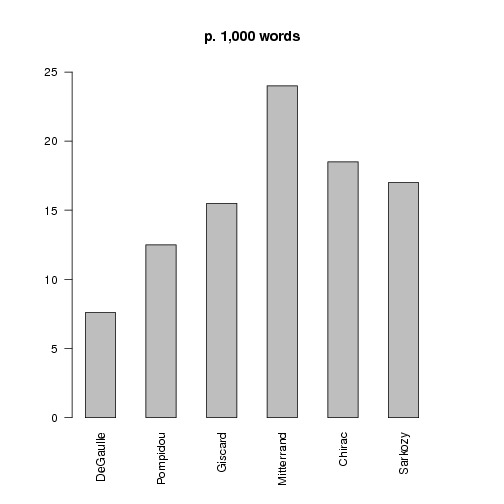
\includegraphics[height=2.5in]{_media/french/je_freq_eng.png} 
%  \caption{Frequency of the use of «~Je~» (``I'') in their talks by several French Presidents}
%  \label{fig:je_stats_en}
%\end{center}
%\end{figure*}

\subsection{French in the cyberspace}

French is now very present over the Internet, and ranked
8\raise+.5ex\hbox{th} (see figure \ref{fig:internettop10_en}) at the end
of 2009, with 57 million users in the world~\cite{internettop10}.

\begin{figure*}[ht]
\begin{center}
 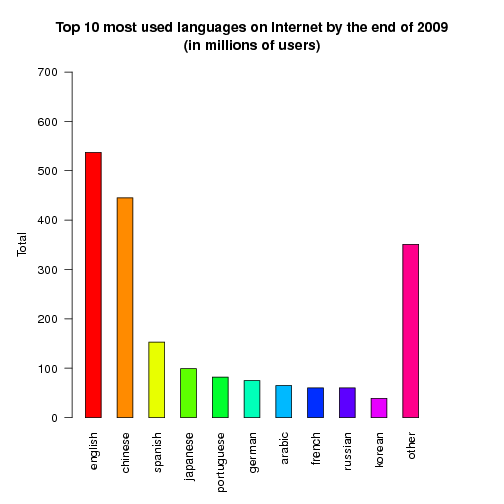
\includegraphics[height=4.0in]{_media/french/french_pix2_top_10_Internet_languages_2010_english.png}
  \caption{Top 10 languages on the Internet by the end of 2009 (in millions of users)~\cite{internettop10}}
  \label{fig:internettop10_en}
\end{center}
\end{figure*}

Collaborative free encyclopedia projects like Wikipedia receive a
strong French contribution (1.19 million articles in January 2012),
next to the German contribution (1.34 million articles), but well behind the English contribution (3.84 million articles)~\cite{wikipediastats}.

A law on accessibility has been voted in 2005 which makes it mandatory
to provide access to information for the disabled, with an extension
to Digital information (e-Accessibility) in 2009~\cite{loi}. This would request
the use of transmedia Language Technologies, such as speech synthesis
for the blind, or sign language generation for the deaf.

\subsection{What is the weight of French?}

Several studies have been conducted on the place of the French
language in the world. In the book {\em Le poids des
langues} (The Weight of Languages)~\cite{calvet09}, A. Calvet and
L.J. Calvet propose to define an index for measuring that weight,
which could include the number of speakers, as a first or second
language, the number of foreign speakers, the number of countries
where it is an official language, the number of translations (as
source or target language), the presence of the language on the
cyberspace (content and access), but also the number of books
published or the number of Nobel prizes in literature. Needless to say
that French gets a good ranking according to this index, second to
English.

\subsection{No multilingualism without Language Technologies}

French has the status of an international language, even though it
loosed a lot of its supremacy with the raise of English (or Globish
(Global English)), as the international ``Lingua Franca'' (!). It still
appears as an official language in many countries and many
international organizations. However, with globalization, the
supremacy of English may result in a monopolistic position in economy
and culture, which has strong political consequences. Many meetings
are now conducted in English, and many documents are produced in
English as the single language. Some French industrial groups ask
their employees to speak English and write in English, and some Higher
Education courses are taught in English. The salvation of French, just
as for many other languages, goes through multilingualism which can at
the same time preserve the individual cultures and allow for
communicating among people speaking different languages. However, the
cost of multilingualism is huge, both in terms of financing and in
terms of workload. Language Technologies may appear as the only way to
allow for multilingualism, by cutting costs and workload, and to save
endangered languages, including French in the long term.

\subsection{The French language over the world}
\label{frenchLanguageInTheWorldEn}
The French language is spoken in many countries all over the world~\cite{francaisautourmonde}.
\begin{center}
{\bf {\sc Europe}}
\end{center}

{\bf Andorra}\\
Catalan is the only official language of Andorra; however, French is
commonly used because of the proximity to France.

{\bf Belgium}\\ 
In Belgium, French is the official language of Wallonia (excluding the
East Cantons, which are German-speaking) and one of the two official
languages - along with Flemish - of the Brussels-Capital Region.

{\bf Italy}\\
French is an official language, along with Italian, in the small region of Aosta Valley in Italy.

{\bf Luxemburg}\\
French is one of the three official languages of the Grand Duchy of Luxembourg, alongside German and Luxembourgish.

{\bf Monaco}\\ 
Although Monegasque is the national language of the Principality of
Monaco, French is the only official language.

{\bf Switzerland}\\
French is one of the four official languages of Switzerland (along with German, Italian and Romansh).

{\bf The United-Kingdom and the Channel islands}\\
French is an official language in both Jersey and Guernsey.

\begin{center}
{\sc North \& South America}
\end{center}

{\bf Canada}\\
French is the second most common language in Canada, after English,
and both are official languages at the federal level. French is the
sole official language in the province of Québec, being the mother
tongue for some 6 million people. New Brunswick, where about a third
of the population is francophone, is the only officially bilingual
province. Portions of Eastern Ontario, North-eastern Ontario, Nova
Scotia and Manitoba have sizable French minorities, but its
prescription as an official language in those jurisdictions and the
level of francophone services vary. Smaller pockets of French speakers
exist in all other provinces.

{\bf Haïti}\\
French is one of Haiti's two official languages, with Haitian Creole. 

{\bf French overseas departments and territories in the Americas}\\
French is also the official language in France's overseas departments and territories of French Guiana, Guadeloupe, Martinique, Saint Barthélémy, St. Martin and Saint-Pierre et Miquelon.

{\bf The United States }\\
French is the fourth most-spoken language in the United States, after
English, Spanish and Chinese, and the second most-spoken in the states
of Louisiana, Maine, Vermont and New Hampshire. Louisiana is home to
many distinct dialects, of which Cajun French has the largest number
of speakers. According to the 2000 US Census, there are over 194,000
people in Louisiana who speak French at home.

{\bf Brazil}\\
The French language in Brazil was spoken for a brief period during the
colonial attempts of France Antarctique and France Equinoctiale. Today
the Karipuna indigenous community (nearly 30,000 people) of Amapá in
North Brazil speaks a French creole, the Lanc-Patuá, possibly related
to the French Guiana Creole.

\begin{center}
{\sc Africa}
\end{center}

A majority of the world's French-speaking population lives in
Africa. According to the 2007 report by the {\em Organisation
internationale de la Francophonie}, an estimated 115 million African
people spread across 31 Francophone African countries can speak French
as either a first or a second language. Due to the rise of French in
Africa, the total French-speaking population is expected to reach 700
million people in 2050.

French is an official language in many African countries, most of them
former French or Belgian colonies: Benin, Burkina Faso, Burundi,
Cameroon, Central African Republic, Chad, Comoros, Republic of the
Congo, Côte d'Ivoire, Democratic Republic of the Congo, Djibouti,
Equatorial Guinea, Gabon, Guinea, Madagascar, Mali, Niger, Rwanda,
Senegal, Seychelles, Togo.

In addition, French is an administrative language and commonly used,
though not on an official basis, in Mauritius and in the Maghreb
states: Algeria, Mauritania, Morocco and Tunisia.

{\bf French overseas departments and territories in Africa}\\
French is also the official language of Mayotte and La Réunion, two
overseas territories of France located in the southwest Indian Ocean.

\begin{center}
{\sc Asia}
\end{center}

{\bf Southwest Asia}\\ 
Arabic is the official language of Lebanon, while a special law shall
regulate the use of French. French is considered a second language by
the Lebanese people and is widely used, especially for administrative
purposes. It is taught in many schools as a secondary language along
with Arabic and English. Like Lebanon, French was official in Syria
until 1943. There are also a significant number of native and
second-language French-speakers in Israel.

{\bf Southeast Asia }\\
French is an administrative language in Laos and Cambodia, although
its influence has waned in recent year. In colonial Vietnam, the
elites spoke French, and many who worked for the French spoke a French
creole known as ``TâBôi'' (now extinct). The language was also spoken
by the elite in the leased territory of Guangzhouwan in southern
China.

{\bf India}\\
French has de jure official status in the Indian Union Territory of
Pondicherry, along with the regional languages Tamil and
Telugu. French is also taught in schools in Chandannagar (a former
French colony in West Bengal).

\begin{center}
{\sc Oceania/Australasia}
\end{center}
French is an official language of the Pacific Island nation of Vanuatu
where 45\% of the population can speak French. In the French territory
of New Caledonia, 97\% of the population can speak, read and write
French. In the French territory of Wallis and Futuna, 78\% of the
population can speak, read and write French.

\subsection{The languages spoken in France}
\label{languageSpokenInTheFranceEn}
Many different languages are spoken in France~\cite{languesparleesfrance}.

{\bf Metropolitan France}\\
{\em Regional languages}: Alsacien, Basque, Breton, Catalan, Corse, Flamand occidental, Francique mosellan, Franco-provençal, Langues d'oïl (Franc-comtois, Wallon, Champenois, Picard, Normand, Gallo, Poitevin-saintongeais [in two varieties: Poitevin and Saintongeais], Lorrain, Bourguignon-morvandiau), ``Parlers'' d'oc or Occitan (Gascon, Languedocien, Provençal, Auvergnat, Limousin, Vivaro-alpin).

{\em Non-territorial Languages}: dialectal Arabic, occidental Armenian, Berber, Judeo-Spanish, Romani, Yiddish.

{\bf Overseas}\\
\textbf{ \emph{Caribbean zone}}:\\
{\em Creole with French lexical basis}: Guadeloupéen, Guyanais, Martiniquais.
{\em Creole bushinenge in Guyane (with anglo-portuguese lexical basis)}: Saramaca, Aluku, Njuka, Paramaca.
{\em Amerindian Languages in Guyana}: Galibi (or Kalina), Wayana, Palikur, Arawak (or Iokono), Wayampi, Emerillon ; Hmong.

{\bf La Réunion}:\\
Reunionian creole  (french lexical basis).

{\bf Nouvelle Calédonie}:\\
28 kanak languages .\\
{\em Grande Terre}: Nyelâyu, Kumak, Caac, Yuaga, Jawe, Nemi, Fwâi, Pije, Pwaamei, Pwapwâ, Voh-Koné language, Cèmuhi, Paicî, Ajië, Arhâ, Arhö, ôrôwe, Neku, Sîchë, Tîrî, Xârâcùù, Xaragurè, Drubéa, Numèè. \\
{\em Loyauté islands}: Nengone, Drehu, Iaai, Fagauvea.

{\bf French Polynesia}:\\
Tahitian, Marquisian, Tuamotu languages, Mangarevian language, Austral Islands languages: Ra'ivavae language, Rapa, Ruturu.

{\bf Wallis and Futuna islands}:\\
Wallisian, Futunian.

{\bf Mayotte}:\\
Maore, Malagasy of Mayotte.

{\bf French Sign Language (FSL)}\\

\end{multicols}

\clearpage

\ssection[Language Technology Support for French]{Language Technology Support\newline for French}

\begin{multicols}{2}

\subsection{Language Technologies}
Language technologies are information technologies that are
specialised for dealing with human language. Therefore these
technologies are also often subsumed under the term Human Language
Technologies. Human language occurs in spoken, written and signed
forms. Whereas speech is the oldest and most natural mode of language
communication, complex information and most of human knowledge is
maintained and transmitted in written texts. Speech and text
technologies process or produce language in these two modes of
realization. But language also has aspects that are shared between
speech and text such as dictionaries, most of grammar and the meaning
of sentences. Thus large parts of language technology cannot be
subsumed under either speech or text technologies. Among those are
technologies that link language to knowledge. Figure \ref{fig:languagetechnoEng} 
illustrates the Language Technology landscape. In our communication,
we mix language with other modes of communication and other
information media. We combine speech with gesture and facial
expressions. Digital texts are combined with pictures and
sounds. Movies may contain language in spoken and written form. Thus
speech and text technologies overlap and interact with many other
technologies that facilitate processing of multimodal communication
and multimedia documents. Sign language allows hearing impaired people to communicate.

\begin{figure*}[htb]
 \colorrule{grey3}{\textwidth}{1.5pt}
\begin{center}
 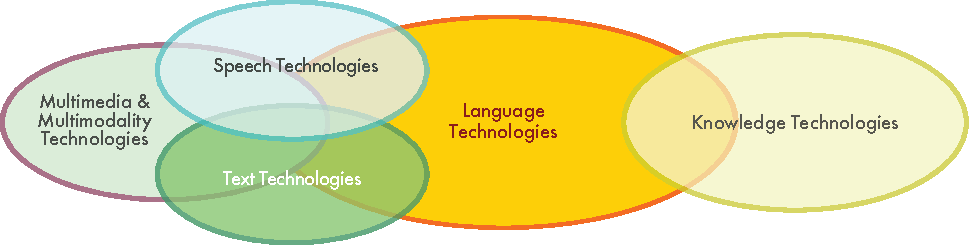
\includegraphics[width=\textwidth]{../_media/english/language_technologies} 
\caption{Language Technologies}
\label{fig:languagetechnoEng}
\end{center}
 \colorrule{grey3}{\textwidth}{1.5pt}
\end{figure*}

\subsection{Language Technology Application Architectures}

Typical software applications for language processing consist of
several components that mirror different aspects of language and of
the task they implement. Figure \ref{fig:textprocarchiEng} displays a highly
simplified architecture that can be found in a text processing
system. The first three modules deal with the structure and meaning of
the text input:
\begin{itemize}
\item Pre-processing: cleaning up the data, removing formatting,
  detecting the input language, etc.
\item Grammatical analysis: finding the verb and its objects,
  modifiers, etc.; detecting the sentence structure.
\item Semantic analysis: disambiguation (Which meaning of ``apple'' is the
  right one in a given context?), resolving anaphora and referring
  expressions like ``she'', ``the car'', etc.; representing the meaning of the
  sentence in a machine-readable way.
\end{itemize}

Task-specific modules then perform many different operations such as
automatic summarization of an input text, database look-ups and many
others. Below, we will illustrate core application areas and highlight
their core modules. Again, the architectures of the applications are
highly simplified and idealised, to illustrate the complexity of
Language Technology (LT) applications in a generally understandable
way.



After introducing the core application areas, we will give a short
description of the situation regarding LT for French, with an overview
of past and on-going research programs. At the end of this section, we
will present an estimate of the situation regarding core LT tools and
resources on a number of dimensions such as availability, maturity, or
quality. This table intends to give a gross and global overview on the
situation of LT for French.

\subsection{Core application areas}

\subsubsection{Language Checking}
Anyone using a word processing tool such as Microsoft Word has come
across a spell-checking component that indicates spelling mistakes and
proposes corrections. 40 years after the first spelling correction
program by Ralph Gorin, language checkers nowadays (see figure
\ref{fig:spellcheckerEn}) do not simply compare the list of extracted
words against a dictionary of correctly spelled words, but have become
increasingly sophisticated. In addition to language-dependent
algorithms for handling morphology (e.\,g. plural formation), some are
now capable of recognizing simple syntax-related errors, such as a
missing verb or a verb that does not agree with its subject in person
and number, e.\,g. in ``She *write a letter.''

However, for other common error types the currently used methods are
not sufficient. For example, take a look at the following first verse
of a poem by Jerrold H. Zar (1992):
%\begin{it}
\begin{quote}
{\em Eye have a spelling chequer,\\
It came with my Pea Sea.\\
It plane lee marks four my revue\\
Miss Steaks I can knot sea.}
\end{quote}
%\end{it}
Most available spell checkers (including Microsoft Word) will find
no errors in this poem because they mostly look at words in
isolation. However, for detecting so-called homophone errors
(e.\,g. ``Eye'' instead of ``I''), the language checker needs to consider
the context in which a word occurs.

\begin{figure*}[htb]
 \colorrule{grey3}{\textwidth}{1.5pt}
\begin{center}
 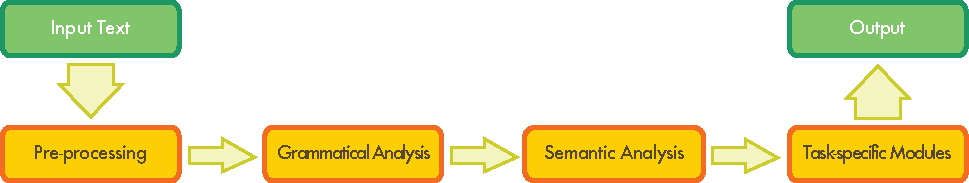
\includegraphics[width=\textwidth]{../_media/english/text_processing_app_architecture}
\caption{Typical text processing pipeline}
\label{fig:textprocarchiEng}
\end{center}
 \colorrule{grey3}{\textwidth}{1.5pt}
\end{figure*}

This either requires the formulation of language-specific {\bf grammar
rules}, i.\,e. a high degree of expertise and manual labour, or the use
of a {\bf statistical language model} to calculate the probability of a
particular word occurring along with the preceding and following
words. For a statistical approach, usually based on n-grams, a large
amount of language data (i.\,e. a {\bf corpus}) is required to obtain
sufficient statistical information.  

Up to now, these approaches have mostly been developed and evaluated
on English language data. However, they do not necessarily transfer
well to other languages, e.\,g. highly inflectional ones or languages
with a flexible word order like German. For these more complex
languages, an advanced high-precision language checker may require the
development of more sophisticated methods, involving a deeper
linguistic analysis.

Language checking is not limited to word processors; it is also used
in ``{\bf authoring support systems}'', i.\,e., software environments in which
manuals and other documentation are written to special standards for
complex IT, healthcare, engineering and other products. Fearing
customer complaints about incorrect use and damage claims resulting
from poorly understood instructions, companies are increasingly
focusing on the quality of technical documentation while targeting the
international market (via translation or localization) at the same
time. Advances in natural language processing have led to the
development of authoring support software, which helps the writer of
technical documentation use vocabulary and sentence structures that
are consistent with industry rules and (corporate) terminology
restrictions, or that are simple in order to facilitate understanding
by non-native speakers or translation.

Besides spell checkers and authoring support, language checking is
also important in the field of computer-assisted language
learning. And language checking applications also automatically
correct search engine queries, as found in Google's ``{\em Did you mean...?}''
suggestions.

In France, Synapse Développement markets the advanced Cordial spelling
and grammatical checker for French (available online on Reverso
website), besides the spell-checkers Antidote of Druide Informatique
and Prolexis of Éditions Diagonal.

\begin{figure*}[!ht]
 \colorrule{grey3}{\textwidth}{1.5pt}
\begin{center}
  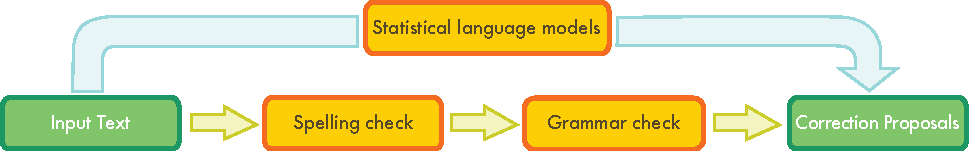
\includegraphics[width=\textwidth]{../_media/english/language_checking}
\caption{Typical architecture for a rule based (yellow arrows) or statistical (blue arrow) spell-checker}
\label{fig:spellcheckerEn}
\end{center}
 \colorrule{grey3}{\textwidth}{1.5pt}
\end{figure*}

\subsubsection{Web search}
The Google search engine (see figure \ref{fig:archiwebEn} for a
typical architecture), which started in 1998, is nowadays used for
about 80\% of all search queries worldwide~\cite{googleworld}, and is
also very popular in France. Neither the search interface nor the
presentation of the retrieved results has significantly changed since
the first version. In the current version, Google offers a spelling
correction for misspelled words and also, in 2009, incorporated basic
semantic search capabilities into their algorithmic mix~\cite{googlesemantics}, which can
improve search accuracy by analysing the meaning of the query terms in
context. The success story of Google shows that with a lot of data at
hand and efficient techniques for indexing these data, a mainly
statistically based approach can lead to satisfactory results.

However, for a more sophisticated information need, integrating deeper
linguistic knowledge is essential. In particular, if a search query
consists of a question or a complete sentence rather than a list of
keywords, retrieving relevant answers to this query requires an
analysis of this question or sentence on a syntactic and semantic
level as well as the availability of an index that allows for a fast
retrieval of relevant documents.



For example, imagine a user inputs the query ``Give me a list of all
companies that were taken over by other companies in the last five
years''. A simple keyword-based approach will not take us very far
here.

Expanding the query terms by synonyms, for example using an
ontological language resource like the Princeton WordNet, may improve
the results. However, for a satisfactory answer, a deeper query
analysis is necessary. For example, applying a syntactic parser to
analyse the grammatical structure of the sentence, we can determine
that the user is looking for companies that have been taken over and
not companies that took over others. We also need to process the
expression ``last five years'' to find out which years it refers to.

Finally, the processed query needs to be matched to a massive amount
of unstructured data in order to find the piece or pieces of
information the user is looking for. This involves the {\bf retrieval and
ranking} of relevant documents. In addition, generating a list of
companies, we also need to extract the information that a particular
string of words in a document refers to a company name. This kind of
information is tagged using a {\bf Named-entity} recogniser.

We face an additional challenge if we want to match a query to
documents written in a different language. For {\bf crosslingual search}, we
have to automatically translate the query to all possible source
languages and map the retrieved information back to the target
language. Again, this requires a linguistic analysis of all texts
involved.

For users with a very specialised information need, an expansion of
the query may require additional knowledge resources like a
domain-specific ontology, representing the concepts relevant within
the domain and the relationships between those concepts.

The increasing share of data available in non-textual format also
drives the demand for services enabling {\bf multimedia search}, i.\,e.,
information search on images, audio and video data. For audio and
video files, this involves a {\bf speech recognition} module to convert
speech content into text or a phonetic representation, to which user
queries can be matched.

In France, the Exalead company successfully developed and demonstrated
in 2010 the {\em Voxalead News}~\cite{voxaleadnews} multimedia search
application in 6 languages (French, English, Spanish, Chinese
Mandarin, Arabic and Russian), slightly ahead of Google.

\begin{figure*}[!ht]
 \colorrule{grey3}{\textwidth}{1.5pt}
\begin{center}
 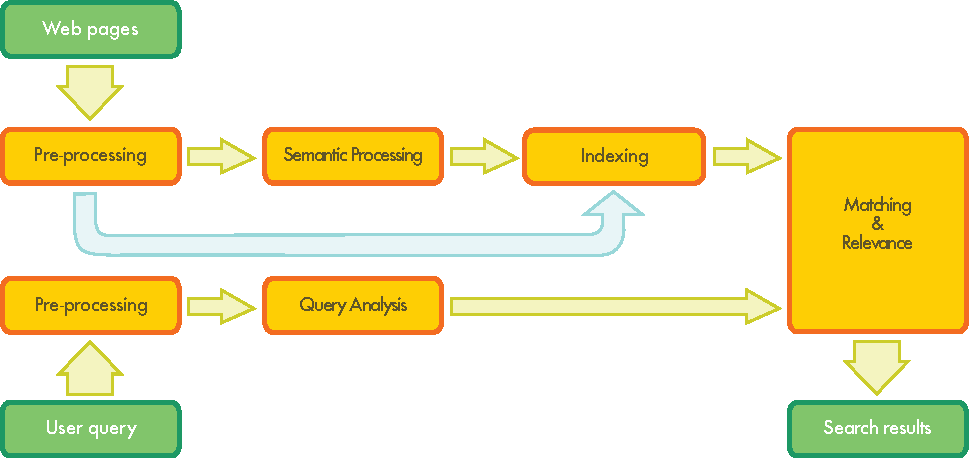
\includegraphics[width=\width]{../_media/english/web_search_architecture}
 \caption{Typical Architecture of a Web Search Engine}
\label{fig:archiwebEn}
\end{center}
 \colorrule{grey3}{\textwidth}{1.5pt}
\end{figure*}

\subsubsection{Speech processing} 
Spoken Language Processing is part of Language Processing, although
the communities working on Computational Linguistics and on Speech
Communication were initially set apart, the former coming from
Theoretical Computer Science and Artificial Intelligence, and the
latter from Signal Processing and Pattern Recognition.

Spoken Language Technologies cover many different areas such as 
{\bf speech analysis and compression, speech recognition and
  understanding, speech synthesis and generation, oral dialog, speaker
  recognition} (who is speaking?), {\bf spoken language
  identification} (in which language?). They may be used in different
applications: voice command, voice dictation, audio-visual,
conversational or meeting transcription, interactive systems, speech
translation, people identification, personal assistant, etc.

For some applications, for example telephone banking, a speech
recognition component matching a voice pattern against an existing
vocabulary is enough. For other applications, e.\,g. voice dictation or
conversation transcription, more sophisticated software with the
ability to process arbitrary natural speech input is required. For
advanced interactive systems, in-depth linguistic analysis of the
speech input is required.


\begin{figure*}
 \colorrule{grey3}{\textwidth}{1.5pt}
\begin{center}
 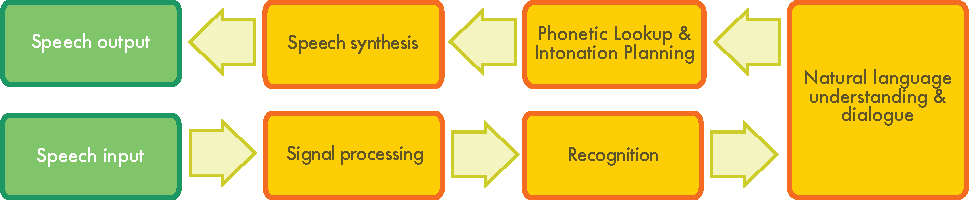
\includegraphics[width=\textwidth]{../_media/english/simple_speech-based_dialogue_architecture} 
\caption{Basic Architecture for a Spoken Language Dialog System}
\label{fig:sldsEng}
\end{center}
 \colorrule{grey3}{\textwidth}{1.5pt}
\end{figure*}

A complete Speech Interaction system comprises the following four
different technologies (see figure \ref{fig:sldsEng}):
\begin{itemize}
\item Automatic speech recognition (ASR) is responsible for
  determining which words were actually spoken given a sequence of
  sounds uttered by the speaker.
\item Syntactic analysis and semantic and pragmatic interpretation
  deal with analysing the syntactic structure of a user's utterance
  and interpreting the latter according to the purpose of the
  respective application.
\item Dialogue management is required for determining, on the part of
  the system the user interacts with, which action shall be taken
  given the user's input and the functionality of the system.
\item Speech synthesis technology is employed for transforming a
  message into sounds that will be output to the listener.
\end{itemize}

ASR systems for a given language are usually based on an {\bf Acoustic
Model}, representing the signal corresponding to the phonemes for that
language, a {\bf Pronunciation Model}, representing the different ways of
pronouncing the words of that language, and a {\bf Language Model},
representing the way words are ordered to produce sentences in that
language. ASR systems based on statistical training approaches
necessitate vast amounts of data (large amounts of transcribed speech
from various speakers with various accents and huge amounts of texts,
reflecting the targeted application) in order to be trained and
achieve sufficient performances.

In spite of major technological advances in the recent years,
currently available ASR systems are still facing difficulty with
{\bf Out-of-Vocabulary words} (OOV): words unknown to the system which make
that the sentences in which they are pronounced are incorrectly
recognised. The vocabulary and Language Model have therefore to be
continuously updated. Another issue is the difficulty for a speech
recognition system, just as other LT, to self-estimate whether a word
or a sentence may have been misunderstood. This problem can be
addressed by assigning a confidence measure to a word or a sentence
that has been recognised.

The expected accuracy rate of the recognition module is highly
dependent on the application. Whereas the user of a dictation system
may usually manually verify and edit the system output, more complex
requirements are imposed on a dialog system intended to naturally
converse with a human. 

This requires:
\begin{itemize} 
\item a deep linguistic analysis of the speech input (i.\,e. {\em
  Named-entity recognition, part-of-speech tagging, co-reference
  resolution, parsing}),
\item but also a {\bf dialog management} component, which uses
  knowledge of the specific task domain to analyse the input on a
  semantic and pragmatic level to generate the appropriate output,
\item and even the handling of {\bf emotion analysis and generation},
  through the processing of prosody (rhythm,stress and intonation),
\item wihtout forgetting the analysis of other {\bf non-verbal
  modalities} (gaze, gestures, facial expression, etc.).
\end{itemize}

The only way to assess the quality of an ASR system is to conduct an
evaluation on test data corresponding to the application. Several
systems based on different approaches may be compared within
evaluation campaigns, such as the ones organised in the US by NIST
(National Institute of Standards and Technology) for DARPA (Defense
Advanced Research Projects Agency) since 1987 (see figure
\ref{fig:nistreco}).

This table shows the progress of Automatic Speech Recognition systems
over the years, through the international evaluation campaigns
conducted by NIST.  The best performance in terms of Word Error Rate
(WER) obtained that year is plotted on this chart using a logarithmic
scale, as the effort to go from 100\% error rate (the system does not
recognize any word) to 10\% being comparable to the one required to go
from 10\% to 1\% error rate. The tasks become increasingly difficult
over the years (first with a voice-activated artificial language of
1,000 words, then Voice dictation (20,000 words), radio/TV Broadcast
News transcriptions (English, Arabic and Chinese Mandarin), telephone
conversations (also in English, Arabic and Mandarin), transcriptions
of meetings, etc.), in variable conditions (real time or not,
different qualities of sound recording, etc.). We see that for some
tasks, the performances of the systems are similar to those of a human
listener, making these systems operational and marketable (such as for
command languages). By cons, it is clear that for more complex tasks,
performances improve more slowly, justifying the continuation of the
research effort. The knowledge of these performances is precious to
determine the feasibility of an application on the basis of the
quality level it requires. For example, an information retrieval
system for audio-visual data does not require very high performances
in the transcription of speech in contrast to spoken dialogue systems
used in critical tasks.

Transforming a message into a speech signal is done by a {\bf speech
synthesis} component. This message can be a text ({\bf Text-to-Speech
Synthesis}, TTS) or the output of an interactive dialog system. Nowadays,
speech synthesis is usually based on large amounts of pre-recorded
speech data in order to produce a reasonably natural result. However,
for the ultimate aim of automatically producing natural speech in
interactive systems, more research is needed, in particular concerning
the interrelation between syntax, semantics, pragmatics and prosody,
and between verbal and non-verbal modalities (facial expression of
artificial {\bf talking faces}, pointing, etc.).

\begin{figure*}[!ht]
\begin{center}
  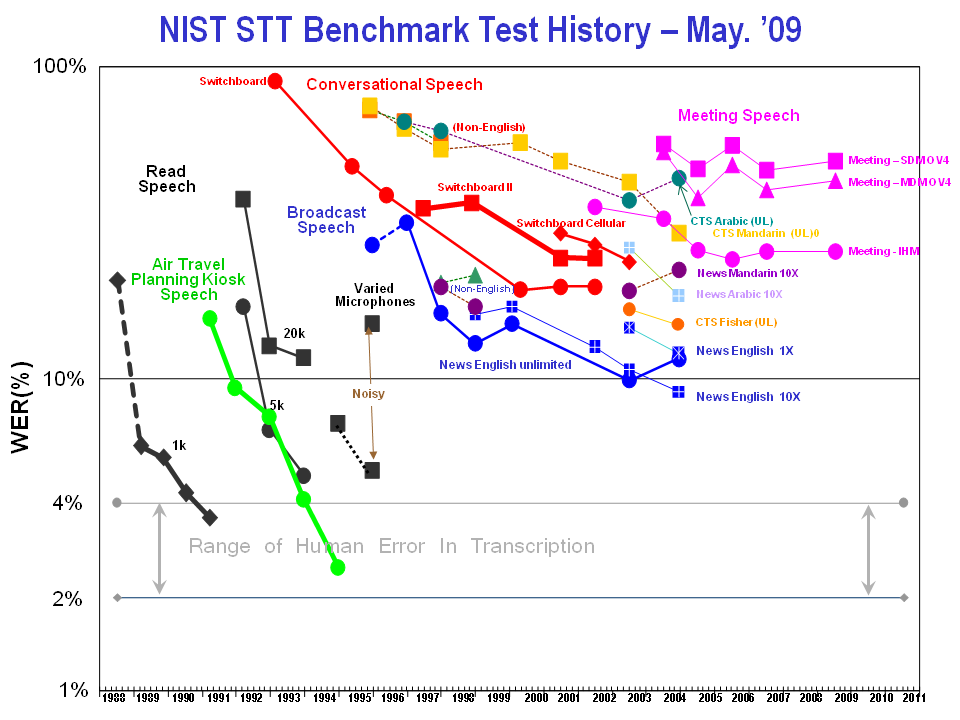
\includegraphics[height=4.0in]{_media/french/french_pix8_speech_reco_nist.png}
  \caption{The history of Automatic Speech Recognition since 1987 through the NIST evaluation campaigns~\cite{speechreconist}}
  \label{fig:nistreco}
\end{center}
\end{figure*}

The French language presents specificities that make it more difficult
to handle by automatic speech processing systems, compared with other
roman languages such as Italian or Spanish. Homophones heterographs
(also called homonyms) raise problems for speech transcription
(phoneme-to-grapheme transcription), and this is often the case for
the mark of plural in French (``s'' for names, ``nt'' for verbs), which is
not pronounced, or is pronounced as a liaison between
words. Homographs heterophones raise problems for grapheme-to-phoneme
transcription in Text-to-Speech Synthesis, which may need syntactic
({\em Les poules du couvent couvent} (``The convent hens incubate eggs'',
pronounced /lepuldykuvãkuv/) or even semantic analysis in some very
few cases ({\em fils} (``sons''), pronounced /fis/ and {\em fils} (``threads''),
pronounced /fil/).

A key issue for future research is the {\bf personalization} of interactive
systems. To some degree, this is already possible, for example in
speech transcription systems, which can also recognize the genre, age,
accent or identity ({\bf diarization}) of the person who is speaking, and in
dictation systems or car navigation systems, which can be trained to
adapt to the user's speaking style. The user-friendly design of dialog
systems is especially important in assistive systems, e.\,g. for
handicapped or elderly people, who may have inhibitions against using
computer systems. This will involve an analysis of human speech
behaviour in general and in particular of the way humans interact with
computers.

Other aspects of speech processing concern {\bf speaker verification or
identification}, for biometrics applications, and {\bf language or dialect
identification}, aiming at identifying which language is spoken.

In times where European and international markets are growing
together, an important challenge for interactive systems is the
ability to work in a multilingual environment, which involves the
{\bf automatic translation of speech} into other languages. First results
have been demonstrated in April 2007 within the EC TC-STAR\cite{tcstarurl} project
for English to Spanish translation of talks at the European
Parliament, taking advantage of the existence of large amounts of
parallel corpora (the talks of the parliamentarians, their
interpretations in all EU official languages, their transcriptions and
the translations of the transcription, also in all EU languages). The
corresponding technology has been implemented on the Jibbigo\cite{jibbigo} system
available in 2011 for 8 language pairs on Apple {\em App Store}. Google offers
in 2011 speech recognition for 17 source languages and speech synthesis
for 25 target languages (including French), in its Google Translate
smartphone application covering 3,300 language pairs, also available
on the {\em App Store}.

The quality of Interactive Speech Translation still needs to be much
improved for it to be of common use in everyday life. Similarly, oral
dialog systems are presently only available for very constrained
applications. However many applications can be addressed with the
presently available technology, such as video {\bf close captioning}
and approximate translation.

Looking beyond today's state of technology, there will be
significant changes due to the spread of smartphones as a new platform
for managing customer relationships - in addition to the telephone,
Internet, and email channels. This tendency will also affect the
employment of technology for Speech Interaction. On the one hand,
demand for telephony-based {\bf Voice User Interfaces} (VUI) will
decrease, on the long run. On the other hand, the usage of spoken
language as a user-friendly input modality for smartphones will gain
significant importance. This tendency is supported by the observable
improvement of speaker-independent speech recognition accuracy for
speech dictation and voice command services that are already offered
to smartphone users (see for instance Apple Siri or Android Voice
Actions). Given this ``outsourcing'' of the recognition
task to the infrastructure of applications, application-specific
employment of linguistic analysis will gain importance compared to the
present situation.

\subsubsection{Machine Translation}
The idea of using digital computers for translation of natural
languages came up in 1946 by A. D. Booth and was followed by
substantial funding for research in this area in the 1950s and
beginning again in the 1980s. France was especially very active in
that field, and the first popular book on Machine Translation was
written by a French man (Delavenay, 1957). Nevertheless, Machine
Translation (MT) still fails to fulfil the high expectations it gave
rise to in its early years.

\begin{figure*}
 \colorrule{grey3}{\textwidth}{1.5pt}
\begin{center}
 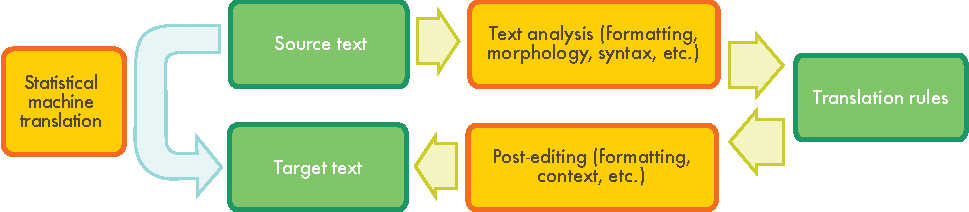
\includegraphics[width=\textwidth]{../_media/english/machine_translation}
\caption{Machine Translation Architecture statistical (blue arrow) or rule based (yellow arrows)}
\label{fig:mtarchiEng}
\end{center}
 \colorrule{grey3}{\textwidth}{1.5pt}
\end{figure*}

At its basic level, MT simply substitutes words in one natural
language by words in another. This can be useful in subject domains
with a very restricted, formulaic language, e.\,g., weather
reports. However, for a good translation of less standardised texts,
larger text units (phrases, sentences, or even whole passages) need to
be matched to their closest counterparts in the target language. The
major difficulty here lies in the fact that human language is
ambiguous, which yields challenges on multiple levels, e.\,g., {\bf word
sense disambiguation} at the lexical level (``bank'' can mean a financial institution or the edge of a river) or the attachment of prepositional phrases on the syntactic
level as in:
\begin{tabular}{l}
\\
Le policier observait l'homme avec ses jumelles.\\
$[${\em The policeman observed the man with his binoculars.}$]$\\
Le policier observait l'homme avec son revolver.\\
$[${\em The policeman observed the man with his revolver.}$]$\\
\\
\end{tabular}

One way of approaching the task is based on linguistic rules (see figure \ref{fig:mtarchiEng}). For
translations between closely related languages, a direct translation
may be feasible in cases like the example above. But often {\bf rule-based}
(or {\bf knowledge-driven}) systems analyse the input text and create an
intermediary, symbolic representation, from which the text in the
target language is generated. The success of these methods is highly
dependent on the availability of extensive {\bf lexicons} with
morphological, syntactic, and semantic information, and large sets of
{\bf grammar} rules carefully designed by a skilled linguist.

Introduced in the late 1980s by researchers coming from the speech
recognition community, as computational power increased and became
less expensive, more interest was shown in {\bf statistical models} for
MT. The parameters of these statistical models are derived from the
analysis of {\bf bilingual text corpora}, such as the Europarl {\bf parallel
corpus}, which contains the proceedings of the European Parliament in
21 European languages. Given enough data, statistical MT works well
enough to derive an approximate meaning of a foreign language
text. However, more than knowledge-driven systems, statistical (or
data-driven) MT may generate an ungrammatical output. On the other
hand, besides the advantage that less human effort is required for
grammar writing, data-driven MT can also cover particularities of the
language that go missing in knowledge-driven systems, for example
idiomatic expressions.

{\bf Hybrid approaches} aim at combining knowledge-based and statistical
approaches. This can be done in several ways. One is to use both
knowledge- and data-driven systems and have a selection module decide
on the best output for each sentence. However, for longer sentences,
no result will be perfect. A better solution is to combine the best
parts of each sentence from multiple outputs, which can be fairly
complex, as corresponding parts of multiple alternatives are not
always obvious and need to be aligned. Another challenging approach is
to design a new setup that combines the advantages of the two
paradigms by integrating the good features of each; for example,
making a rule-based system adaptive by adding a module for rule
learning, or making a statistical MT system syntax-aware by adding
syntactic information.

The quality of MT systems is still considered to have huge improvement
potential. Challenges include the adaptability of the language
resources to a given subject domain or user area and the integration
into existing workflows with term bases and translation memories. In
addition, most of the current systems are English-centred and support
only few languages across the other languages. Research in MT has been
conducted for many years without assessing the quality of the produced
translation in order to compare various approaches or measure
progress. The BLEU measure has been proposed in 2000\cite{bleu02}, and allowed for
conducting comparative MT {\bf evaluation campaigns}, even if this simple
measure, based on a word to word comparison between the MT output and
reference human translations, may be criticised for merging the
meaning and the stylistic aspects of a translation. Since then, other
metrics have been proposed and an evaluation campaign of MT {\bf evaluation
metrics} has even been organised by NIST without moving yet to another
fully accepted measure. Such evaluation campaigns allow for comparing
the quality of MT systems, the various approaches and the status of MT
systems for the different languages, as it appears in a Table
presented within the EC Euromatrix+ project (see figure \ref{fig:euromatrixplus}).

% \begin{figure*}[!ht]
% \begin{center}
%   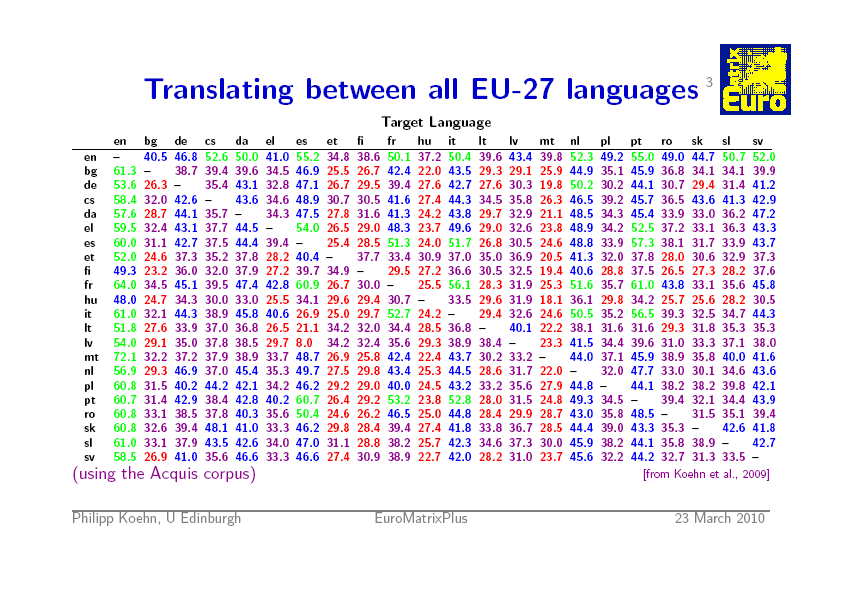
\includegraphics[height=5.0in]{../_media/french/french_table1_mt_matrix.png}
%   \caption{Machine Translation performances (BLEU measure) for a set of language pairs made with 22 EU official languages~\cite{mt462}. Source languages are given in rows and target languages in columns.}
%   \label{fig:euromatrixplus}
% \end{center}
% \end{figure*}

\begin{figure*}[tbp]
  \centering
  \setlength{\tabcolsep}{0.17em}
  \small
  \begin{tabular}{>{\columncolor{corange1}}cccccccccccccccccccccccc}
    & \multicolumn{22}{>{\columncolor{corange1}}c}{\textcolor{red}{Target language (X axis)} -- \textcolor{grey1}{Source Language (Y axis)}}\\\addlinespace[{-.009cm}]
    \rowcolor{corange1}  & EN & BG & DE & CS & DA & EL & ES & ET & FI & FR & HU & IT & LT & LV & MT & NL & PL & PT & RO & SK & SL & SV\\
    EN & -- & \textcolor{blue}{40.5} & \textcolor{blue}{46.8} & \textcolor{green2}{52.6} & \textcolor{green2}{50.0} & \textcolor{blue}{41.0} & \textcolor{green2}{55.2} & \textcolor{purple}{34.8} & \textcolor{purple}{38.6} & \textcolor{green2}{50.1} & \textcolor{purple}{37.2} & \textcolor{green2}{50.4} & \textcolor{purple}{39.6} & \textcolor{blue}{43.4} & \textcolor{purple}{39.8} & \textcolor{green2}{52.3} & \textcolor{blue}{49.2} & \textcolor{green2}{55.0} & \textcolor{blue}{49.0} & \textcolor{blue}{44.7} & \textcolor{green2}{50.7} & \textcolor{green2}{52.0}\\
    BG & \textcolor{green}{61.3} & -- & \textcolor{purple}{38.7} & \textcolor{purple}{39.4} & \textcolor{purple}{39.6} & \textcolor{purple}{34.5} & \textcolor{blue}{46.9} & \textcolor{red3}{25.5} & \textcolor{red3}{26.7} & \textcolor{blue}{42.4} & \textcolor{red3}{22.0} & \textcolor{blue}{43.5} & \textcolor{red3}{29.3} & \textcolor{red3}{29.1} & \textcolor{red3}{25.9} & \textcolor{blue}{44.9} & \textcolor{purple}{35.1} & \textcolor{blue}{45.9} & \textcolor{purple}{36.8} & \textcolor{purple}{34.1} & \textcolor{purple}{34.1} & \textcolor{purple}{39.9}\\
    DE & \textcolor{green2}{53.6} & \textcolor{red3}{26.3} & -- & \textcolor{purple}{35.4} & \textcolor{blue}{43.1} & \textcolor{purple}{32.8} & \textcolor{blue}{47.1} & \textcolor{red3}{26.7} & \textcolor{red3}{29.5} & \textcolor{purple}{39.4} & \textcolor{red3}{27.6} & \textcolor{blue}{42.7} & \textcolor{red3}{27.6} & \textcolor{purple}{30.3} & \textcolor{red2}{19.8} & \textcolor{green2}{50.2} & \textcolor{purple}{30.2} & \textcolor{blue}{44.1} & \textcolor{purple}{30.7} & \textcolor{red3}{29.4} & \textcolor{purple}{31.4} & \textcolor{blue}{41.2}\\
    CS & \textcolor{green2}{58.4} & \textcolor{purple}{32.0} & \textcolor{blue}{42.6} & -- & \textcolor{blue}{43.6} & \textcolor{purple}{34.6} & \textcolor{blue}{48.9} & \textcolor{purple}{30.7} & \textcolor{purple}{30.5} & \textcolor{blue}{41.6} & \textcolor{red3}{27.4} & \textcolor{blue}{44.3} & \textcolor{purple}{34.5} & \textcolor{purple}{35.8} & \textcolor{red3}{26.3} & \textcolor{blue}{46.5} & \textcolor{purple}{39.2} & \textcolor{blue}{45.7} & \textcolor{purple}{36.5} & \textcolor{blue}{43.6} & \textcolor{blue}{41.3} & \textcolor{blue}{42.9}\\
    DA & \textcolor{green2}{57.6} & \textcolor{red3}{28.7} & \textcolor{blue}{44.1} & \textcolor{purple}{35.7} & -- & \textcolor{purple}{34.3} & \textcolor{blue}{47.5} & \textcolor{red3}{27.8} & \textcolor{purple}{31.6} & \textcolor{blue}{41.3} & \textcolor{red3}{24.2} & \textcolor{blue}{43.8} & \textcolor{red3}{29.7} & \textcolor{purple}{32.9} & \textcolor{red3}{21.1} & \textcolor{blue}{48.5} & \textcolor{purple}{34.3} & \textcolor{blue}{45.4} & \textcolor{purple}{33.9} & \textcolor{purple}{33.0} & \textcolor{purple}{36.2} & \textcolor{blue}{47.2}\\
    EL & \textcolor{green2}{59.5} & \textcolor{purple}{32.4} & \textcolor{blue}{43.1} & \textcolor{purple}{37.7} & \textcolor{blue}{44.5} & -- & \textcolor{green2}{54.0} & \textcolor{red3}{26.5} & \textcolor{red3}{29.0} & \textcolor{blue}{48.3} & \textcolor{red3}{23.7} & \textcolor{blue}{49.6} & \textcolor{red3}{29.0} & \textcolor{purple}{32.6} & \textcolor{red3}{23.8} & \textcolor{blue}{48.9} & \textcolor{purple}{34.2} & \textcolor{green2}{52.5} & \textcolor{purple}{37.2} & \textcolor{purple}{33.1} & \textcolor{purple}{36.3} & \textcolor{blue}{43.3}\\
    ES & \textcolor{green}{60.0} & \textcolor{purple}{31.1} & \textcolor{blue}{42.7} & \textcolor{purple}{37.5} & \textcolor{blue}{44.4} & \textcolor{purple}{39.4} & -- & \textcolor{red3}{25.4} & \textcolor{red3}{28.5} & \textcolor{green2}{51.3} & \textcolor{red3}{24.0} & \textcolor{green2}{51.7} & \textcolor{red3}{26.8} & \textcolor{purple}{30.5} & \textcolor{red3}{24.6} & \textcolor{blue}{48.8} & \textcolor{purple}{33.9} & \textcolor{green2}{57.3} & \textcolor{purple}{38.1} & \textcolor{purple}{31.7} & \textcolor{purple}{33.9} & \textcolor{blue}{43.7}\\
    ET & \textcolor{green2}{52.0} & \textcolor{red3}{24.6} & \textcolor{purple}{37.3} & \textcolor{purple}{35.2} & \textcolor{purple}{37.8} & \textcolor{red3}{28.2} & \textcolor{blue}{40.4} & -- & \textcolor{purple}{37.7} & \textcolor{purple}{33.4} & \textcolor{purple}{30.9} & \textcolor{purple}{37.0} & \textcolor{purple}{35.0} & \textcolor{purple}{36.9} & \textcolor{red3}{20.5} & \textcolor{blue}{41.3} & \textcolor{purple}{32.0} & \textcolor{purple}{37.8} & \textcolor{red3}{28.0} & \textcolor{purple}{30.6} & \textcolor{purple}{32.9} & \textcolor{purple}{37.3}\\
    FI & \textcolor{blue}{49.3} & \textcolor{red3}{23.2} & \textcolor{purple}{36.0} & \textcolor{purple}{32.0} & \textcolor{purple}{37.9} & \textcolor{red3}{27.2} & \textcolor{purple}{39.7} & \textcolor{purple}{34.9} & -- & \textcolor{red3}{29.5} & \textcolor{red3}{27.2} & \textcolor{purple}{36.6} & \textcolor{purple}{30.5} & \textcolor{purple}{32.5} & \textcolor{red2}{19.4} & \textcolor{blue}{40.6} & \textcolor{red3}{28.8} & \textcolor{purple}{37.5} & \textcolor{red3}{26.5} & \textcolor{red3}{27.3} & \textcolor{red3}{28.2} & \textcolor{purple}{37.6}\\
    FR & \textcolor{green}{64.0} & \textcolor{purple}{34.5} & \textcolor{blue}{45.1} & \textcolor{purple}{39.5} & \textcolor{blue}{47.4} & \textcolor{blue}{42.8} & \textcolor{green}{60.9} & \textcolor{red3}{26.7} & \textcolor{purple}{30.0} & -- & \textcolor{red3}{25.5} & \textcolor{green2}{56.1} & \textcolor{red3}{28.3} & \textcolor{purple}{31.9} & \textcolor{red3}{25.3} & \textcolor{green2}{51.6} & \textcolor{purple}{35.7} & \textcolor{green}{61.0} & \textcolor{blue}{43.8} & \textcolor{purple}{33.1} & \textcolor{purple}{35.6} & \textcolor{blue}{45.8}\\
    HU & \textcolor{blue}{48.0} & \textcolor{red3}{24.7} & \textcolor{purple}{34.3} & \textcolor{purple}{30.0} & \textcolor{purple}{33.0} & \textcolor{red3}{25.5} & \textcolor{purple}{34.1} & \textcolor{red3}{29.6} & \textcolor{red3}{29.4} & \textcolor{purple}{30.7} & -- & \textcolor{purple}{33.5} & \textcolor{red3}{29.6} & \textcolor{purple}{31.9} & \textcolor{red2}{18.1} & \textcolor{purple}{36.1} & \textcolor{red3}{29.8} & \textcolor{purple}{34.2} & \textcolor{red3}{25.7} & \textcolor{red3}{25.6} & \textcolor{red3}{28.2} & \textcolor{purple}{30.5}\\
    IT & \textcolor{green}{61.0} & \textcolor{purple}{32.1} & \textcolor{blue}{44.3} & \textcolor{purple}{38.9} & \textcolor{blue}{45.8} & \textcolor{blue}{40.6} & \textcolor{red3}{26.9} & \textcolor{red3}{25.0} & \textcolor{red3}{29.7} & \textcolor{green2}{52.7} & \textcolor{red3}{24.2} & -- & \textcolor{red3}{29.4} & \textcolor{purple}{32.6} & \textcolor{red3}{24.6} & \textcolor{green2}{50.5} & \textcolor{purple}{35.2} & \textcolor{green2}{56.5} & \textcolor{purple}{39.3} & \textcolor{purple}{32.5} & \textcolor{purple}{34.7} & \textcolor{blue}{44.3}\\
    LT & \textcolor{green2}{51.8} & \textcolor{red3}{27.6} & \textcolor{purple}{33.9} & \textcolor{purple}{37.0} & \textcolor{purple}{36.8} & \textcolor{red3}{26.5} & \textcolor{red3}{21.1} & \textcolor{purple}{34.2} & \textcolor{purple}{32.0} & \textcolor{purple}{34.4} & \textcolor{red3}{28.5} & \textcolor{purple}{36.8} & -- & \textcolor{blue}{40.1} & \textcolor{red3}{22.2} & \textcolor{purple}{38.1} & \textcolor{purple}{31.6} & \textcolor{purple}{31.6} & \textcolor{red3}{29.3} & \textcolor{purple}{31.8} & \textcolor{purple}{35.3} & \textcolor{purple}{35.3}\\
    LV & \textcolor{green2}{54.0} & \textcolor{red3}{29.1} & \textcolor{purple}{35.0} & \textcolor{purple}{37.8} & \textcolor{purple}{38.5} & \textcolor{red3}{29.7} & \textcolor{red2}{8.0} & \textcolor{purple}{34.2} & \textcolor{purple}{32.4} & \textcolor{purple}{35.6} & \textcolor{red3}{29.3} & \textcolor{purple}{38.9} & \textcolor{purple}{38.4} & -- & \textcolor{red3}{23.3} & \textcolor{blue}{41.5} & \textcolor{purple}{34.4} & \textcolor{purple}{39.6} & \textcolor{purple}{31.0} & \textcolor{purple}{33.3} & \textcolor{purple}{37.1} & \textcolor{purple}{38.0}\\
    MT & \textcolor{green}{72.1} & \textcolor{purple}{32.2} & \textcolor{purple}{37.2} & \textcolor{purple}{37.9} & \textcolor{purple}{38.9} & \textcolor{purple}{33.7} & \textcolor{blue}{48.7} & \textcolor{red3}{26.9} & \textcolor{red3}{25.8} & \textcolor{blue}{42.4} & \textcolor{red3}{22.4} & \textcolor{blue}{43.7} & \textcolor{purple}{30.2} & \textcolor{purple}{33.2} & -- & \textcolor{blue}{44.0} & \textcolor{purple}{37.1} & \textcolor{blue}{45.9} & \textcolor{purple}{38.9} & \textcolor{purple}{35.8} & \textcolor{blue}{40.0} & \textcolor{blue}{41.6}\\
    NL & \textcolor{green2}{56.9} & \textcolor{red3}{29.3} & \textcolor{blue}{46.9} & \textcolor{purple}{37.0} & \textcolor{blue}{45.4} & \textcolor{purple}{35.3} & \textcolor{blue}{49.7} & \textcolor{red3}{27.5} & \textcolor{red3}{29.8} & \textcolor{blue}{43.4} & \textcolor{red3}{25.3} & \textcolor{blue}{44.5} & \textcolor{red3}{28.6} & \textcolor{purple}{31.7} & \textcolor{red3}{22.0} & -- & \textcolor{purple}{32.0} & \textcolor{blue}{47.7} & \textcolor{purple}{33.0} & \textcolor{purple}{30.1} & \textcolor{purple}{34.6} & \textcolor{blue}{43.6}\\
    PL & \textcolor{green}{60.8} & \textcolor{purple}{31.5} & \textcolor{blue}{40.2} & \textcolor{blue}{44.2} & \textcolor{blue}{42.1} & \textcolor{purple}{34.2} & \textcolor{blue}{46.2} & \textcolor{red3}{29.2} & \textcolor{red3}{29.0} & \textcolor{blue}{40.0} & \textcolor{red3}{24.5} & \textcolor{blue}{43.2} & \textcolor{purple}{33.2} & \textcolor{purple}{35.6} & \textcolor{red3}{27.9} & \textcolor{blue}{44.8} & -- & \textcolor{blue}{44.1} & \textcolor{purple}{38.2} & \textcolor{purple}{38.2} & \textcolor{purple}{39.8} & \textcolor{blue}{42.1}\\
    PT & \textcolor{green}{60.7} & \textcolor{purple}{31.4} & \textcolor{blue}{42.9} & \textcolor{purple}{38.4} & \textcolor{blue}{42.8} & \textcolor{blue}{40.2} & \textcolor{green}{60.7} & \textcolor{red3}{26.4} & \textcolor{red3}{29.2} & \textcolor{green2}{53.2} & \textcolor{red3}{23.8} & \textcolor{green2}{52.8} & \textcolor{red3}{28.0} & \textcolor{purple}{31.5} & \textcolor{red3}{24.8} & \textcolor{blue}{49.3} & \textcolor{purple}{34.5} & -- & \textcolor{purple}{39.4} & \textcolor{purple}{32.1} & \textcolor{purple}{34.4} & \textcolor{blue}{43.9}\\
    RO & \textcolor{green}{60.8} & \textcolor{purple}{33.1} & \textcolor{purple}{38.5} & \textcolor{purple}{37.8} & \textcolor{blue}{40.3} & \textcolor{purple}{35.6} & \textcolor{green2}{50.4} & \textcolor{red3}{24.6} & \textcolor{red3}{26.2} & \textcolor{blue}{46.5} & \textcolor{red3}{25.0} & \textcolor{blue}{44.8} & \textcolor{red3}{28.4} & \textcolor{red3}{29.9} & \textcolor{red3}{28.7} & \textcolor{blue}{43.0} & \textcolor{purple}{35.8} & \textcolor{blue}{48.5} & -- & \textcolor{purple}{31.5} & \textcolor{purple}{35.1} & \textcolor{purple}{39.4}\\
    SK & \textcolor{green}{60.8} & \textcolor{purple}{32.6} & \textcolor{purple}{39.4} & \textcolor{blue}{48.1} & \textcolor{blue}{41.0} & \textcolor{purple}{33.3} & \textcolor{blue}{46.2} & \textcolor{red3}{29.8} & \textcolor{red3}{28.4} & \textcolor{purple}{39.4} & \textcolor{red3}{27.4} & \textcolor{blue}{41.8} & \textcolor{purple}{33.8} & \textcolor{purple}{36.7} & \textcolor{red3}{28.5} & \textcolor{blue}{44.4} & \textcolor{purple}{39.0} & \textcolor{blue}{43.3} & \textcolor{purple}{35.3} & -- & \textcolor{blue}{42.6} & \textcolor{blue}{41.8}\\
    SL & \textcolor{green}{61.0} & \textcolor{purple}{33.1} & \textcolor{purple}{37.9} & \textcolor{blue}{43.5} & \textcolor{blue}{42.6} & \textcolor{purple}{34.0} & \textcolor{blue}{47.0} & \textcolor{purple}{31.1} & \textcolor{red3}{28.8} & \textcolor{purple}{38.2} & \textcolor{red3}{25.7} & \textcolor{blue}{42.3} & \textcolor{purple}{34.6} & \textcolor{purple}{37.3} & \textcolor{purple}{30.0} & \textcolor{blue}{45.9} & \textcolor{purple}{38.2} & \textcolor{blue}{44.1} & \textcolor{purple}{35.8} & \textcolor{purple}{38.9} & -- & \textcolor{blue}{42.7}\\
    SV & \textcolor{green2}{58.5} & \textcolor{red3}{26.9} & \textcolor{blue}{41.0} & \textcolor{purple}{35.6} & \textcolor{blue}{46.6} & \textcolor{purple}{33.3} & \textcolor{blue}{46.6} & \textcolor{red3}{27.4} & \textcolor{purple}{30.9} & \textcolor{purple}{38.9} & \textcolor{red3}{22.7} & \textcolor{blue}{42.0} & \textcolor{red3}{28.2} & \textcolor{purple}{31.0} & \textcolor{red3}{23.7} & \textcolor{blue}{45.6} & \textcolor{purple}{32.2} & \textcolor{blue}{44.2} & \textcolor{purple}{32.7} & \textcolor{purple}{31.3} & \textcolor{purple}{33.5} & --\\
    \end{tabular}
%  \caption{Performances (mesure BLEU) de Traduction Automatique pour un ensemble de paires de langues constitué à partir de 22 langues officielles de l'Union Européenne~\cite{mt462}. La langue source est donnée en ligne et la langue cible est donnée en colonne.}
 \caption{{Performance of Machine Translation systems between 22 EU-languages~\cite{mt462}}}
 \label{fig:euromatrixplus}
\end{figure*}

This figure gives the best performance obtained for 462 pairs of the
European Union official languages (Irish is missing), in terms of BLEU
score (the higher the score, the better the translation, a human
translator would get around 80). The best results (shown in green and
blue) are the languages that benefit from considerable research
efforts, within coordinated programs, and from the existence of many
parallel corpora (English, French, Dutch, Spanish, German, etc.), the
worst (in red) to languages that did not benefit from similar efforts,
or that are very different from other languages (Hungarian, Maltese,
Finnish, etc.).

France is very active in the area of Machine Translation, with
companies such as Systran, which was a pioneer in this area and
previously provided the technology offered by Google among its
linguistic tools before Google developed and used its own technology,
or Softissimo. Lingua et Machina proposes Translation Memories to
human translators. Several laboratories also conduct research in this
area, achieving state-of-the-art results.

\subsubsection{Other application areas}

Building Language Technology applications involves a range of subtasks
that do not always surface at the level of interaction with the user,
but provide significant service functionalities ``under the hood'' of
the system. Therefore, they constitute important research issues that
have become individual sub-disciplines of Computational Linguistics in
academia.

{\bf Question answering} has become an active area of research, for
which annotated corpora have been built and scientific competitions
have been started. The principle is to move from keyword-based search
(to which the engine responds with a whole collection of potentially
relevant documents) to the scenario of the user asking a concrete
question and the system providing a single answer:

\begin{itemize}
\item[] \textit{- Question: At what age did Neil Armstrong step on the moon?}
\item[] \textit{- Answer: 38.}
\end{itemize}

While this is obviously related to the aforementioned core area
Web Search, question answering nowadays is primarily an umbrella term
for research questions such as: what types of questions should be
distinguished (fact or definition) and how should they be handled?, how
to synthesize an answer from a set of documents that could contain
contradictory information elements about the answer?, or how to extract
the answer from a document belonging to a thematic field other than
the one of the question, but which nevertheless hold the appropriate
information?

This is in turn related to the {\bf information extraction} (IE) task, an
area that was extremely popular and influential at the time of the
'statistical turn' in Computational Linguistics, in the early
1990s. IE aims at identifying specific pieces of information in
specific classes of documents; this could be e.\,g. the detection of the
key players in company takeovers as reported in newspaper
stories. Another scenario that has been worked on is reports on
terrorist incidents, where the problem is to map the text to a
template specifying the perpetrator, the target, time and location of
the incident, and the results of the incident. Domain-specific
template-filling is the central characteristic of IE, which for this
reason is another example of a ``behind the scenes'' technology that
constitutes a well-demarcated research area but for practical purposes
then needs to be embedded into a suitable application environment.

In language technology there exist ``borderline'' areas, which address at the same time standalone applications and supportive, ``under the hood''
components, for instance: {\bf text summarization} and {\bf text
  generation}. Summarization, obviously, refers to the task of making
a long text short, and is offered for instance as a functionality
within MS Word. It works largely on a statistical basis, by first
identifying ``important'' words in a text (that is, for example, words
that are highly frequent in this text but markedly less frequent in
general language use) and then determining those sentences that
contain many important words. These sentences are then marked in the
document, or extracted from it, and are taken to constitute the
summary. In this scenario, which is by far the most popular one,
summarization equals sentence extraction: the text is reduced to a
subset of its sentences. All commercial summarisers make use of this
idea. An alternative approach, to which some research is devoted, is
to actually synthesize new sentences, i.\,e., to build a summary of
sentences that did not show up under that form in the source text. This
requires a certain amount of deeper understanding of the text and
therefore is much less robust. All in all, a text generator is in most
cases not a stand-alone application but embedded into a larger
software environment, such as into the clinical information system
where patient data is collected, stored and processed, and report
generation is just one of many functionalities.

For French, the situation in all these research areas is much less
developed than it is for English, where question answering,
information extraction, and summarization have since the 1990s been
the subject of numerous open competitions, primarily those organised
by DARPA/NIST in the United States. These have significantly improved
the state of the art, but the focus has always been mostly on English
or on languages of geopolitical importance for the US. Some
competitions have added multilingual or crosslingual tracks, such as
the evaluation campaigns conducted within the EC CLEF (Cross-Language
Evaluation Forum)~\cite{clef} project, but French was never
prominent. Accordingly, there are hardly any annotated corpora or
other resources for most of these tasks. Summarization systems, when
using purely statistical methods, are often to a good extent
language-independent, and thus some research prototypes are
available. For text generation, reusable components have traditionally
been limited to the surface realization modules (the ``generation
grammars''); again, most available software is for English.

\subsubsection{Sign Language processing}

Sign Language Processing is a rapidly growing research area, which
goes in connection with the development of the use of Sign Languages
among deaf people, and the legal obligation to provide access to the
information for handicapped people. French Sign Language ({\em Langues des
Signes Françaises} (LSF)) shouldn't be considered as a variant of the
French language, but as a language per se. We will therefore only
mention that Sign Language processing comprises analysis (based on
image processing, and necessitating gesture, facial expression and
posture recognition), generation (in the form of Conversational
Agents) and even translation from one Sign Language to
another. Several laboratories work in France on this research topic,
and first results allowed equipping some French railway stations with
Sign Language information for the deaf.

\subsection{The Technological Effort on French}

\subsubsection{Studies of the Language Technology field for French}

Several studies have been conducted in France in the field of language
technologies, such as the DGLFLF report on the cultural challenges of
Language Technologies in 2007\cite{dglflf07}, the report of the {\em Forum des Droits de
l'Internet} on ``Internet and Sustainable Development: Languages and Internet'' in 2009~\cite{droitsinternet07}, the
European Language Technology market study conducted for the Ministry
of Research by the Bureau Van Dijk in 2007~\cite{vandijk07} or the White Book of the
APIL on Language Industries in 2005~\cite{apil05}. The French Ministry of Culture
and Communication conducted in 2011 a study on the uses and
applications of Language Technologies for French, with a specific
interest on the cultural and economic dimensions.

\subsubsection{The funding}
Funding for research and development in Language Technology mostly
comes from the Ministry of Higher Education and Research through the
National Research Agency (ANR), from the Ministry of Economy, Finance
and Industry through the OSEO Agency and through the {\em Pôles de
Compétitivité} (Competitiveness Clusters), gathering industrials and
researchers, which are funded by several Ministries and by local
administrations (departments and regions). The {\em Direction Générale de
l'Armement} of the Ministry of Defence has its own programs for defence
applications, and also cooperates with the previously mentioned
agencies on cooperative programs regarding dual (civil and defence)
technologies, including Language Technologies.

\subsubsection{The programs}
Research on the French language has been supported by several
programs. The {\em Réseau Francophone d’Ingénierie de la Langue} (FRANCIL)
has been sustained by the Francophone Universities Association
(Aupelf, now AUF) from 1994 to 2000. It contained cooperation projects
between Northern francophone countries and Southern ones (especially
in Africa and Asia) and ``coopetition'' (mixing cooperation and
competition) projects organised as technology evaluation campaigns
both on written and spoken language processing.

The TechnoLangue program (2003-2005)~\cite{technolangue} was
supported by the Ministries of Research, Industry and Culture,
following a report of the {\em Conseil Supérieur de la Langue
  Française}. It included the development of Language Resources
(corpus, lexica, dictionaries, etc.) for French and the organization
of 8 evaluation campaigns, on topics such as Syntactic Parsing,
Machine Translation, Information Retrieval (Question \& Answer) or
Broadcast News speech transcription (ESTER campaign). All data and
tools produced within the evaluation campaigns have been distributed
as Evaluation Packages. It was followed on the same basis by the
TechnoVision program addressing research in Computer Vision,
comprising OCR (Optical Character Recognition) and document processing
(including handwritten character recognition). 

Some of those activities are now
continuing as individual projects supported by the ANR, which
organised the REPERE challenge on multimodal (text, speech and vision)
person identification (2010-2013).

CNRS (the National Centre for Scientific Research) had several
programs in that field along the years either in ICT or in HSS (GRECO,
CCIIL, Silfide (with Aupelf), CRN (including the CNTRL~\cite{cnrtl} and the
CRDO~\cite{crdo}~\cite{crdo2})), and the French Ministry for Research settled in 2011 a
Corpus Infrastructure~\cite{infracorpus} in the Human and Social Sciences area, in
connection with the EC CLARIN project.

Those programs helped a lot in gathering the scientific community
around a common objective and allowed for the production of data
(corpus, lexica, dictionaries...), which are crucial for the development
of technologies. With the help of those efforts, French is ranked 3\raise+.5ex\hbox{rd}
after English and German in terms of the number of Language Resources
devoted to MT available for the European Union official languages, as
it appears in the Euromatrix+~\cite{euromatrixplus} (see figure \ref{fig:EuromatrixRessource}), where 130 resources have been identified for French (May 2011).

%\begin{figure*}
%\begin{center}
%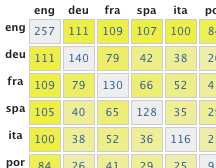
\includegraphics[width=4.0in]{_media/french/french_table2_euromatrix.png}
%\caption{Number of Language Resources for various language pairs including french, according to Euromatrix+}
%\label{fig:EuromatrixFrRessource}
%\end{center}
%\end{figure*}

\begin{figure*}[tbp]
  \centering
  \begin{tabular}{lrrrrrr}
        & English  & German & French & Spanish & Italian & ... \\
    English & \cellcolor{corange5}257 & \cellcolor{corange2}111 & \cellcolor{corange2}109 & \cellcolor{corange2}107 & \cellcolor{corange2}100 &  \cellcolor{corange1} \\     
    German & \cellcolor{corange2}111 & \cellcolor{corange4}140 &  \cellcolor{corange1}79 &  \cellcolor{corange1}42 & \cellcolor{corange1}38 & \cellcolor{corange1}\\     
    French & \cellcolor{corange2}109 & \cellcolor{corange1}79 & \cellcolor{corange3}130 &  \cellcolor{corange1}66 & \cellcolor{corange1}52 & \cellcolor{corange1}\\     
    Spanish & \cellcolor{corange2}105 & \cellcolor{corange1}40 &  \cellcolor{corange1}65 & \cellcolor{corange2}128 & \cellcolor{corange1}35 & \cellcolor{corange1}\\     
    Italian & \cellcolor{corange2}100 & \cellcolor{corange1}38 &  \cellcolor{corange1}52 &  \cellcolor{corange1}36 & \cellcolor{corange2}116 & \cellcolor{corange1}\\     
    ... & \cellcolor{corange1}    & \cellcolor{corange1}    & \cellcolor{corange1}    & \cellcolor{corange1}    & \cellcolor{corange1}    & \cellcolor{corange1}\\
  \end{tabular}
\caption{Number of Language Resources for various language pairs including french, according to Euromatrix+}
\label{fig:EuromatrixRessource}
\end{figure*}

For example, the TechnoLangue ESTER campaign allowed producing, in
2004, 1,700 hours of Broadcast News speech in French, 100 hours of
which have been transcribedi, making it possible to develop Broadcast
News transcription systems of sufficient quality and opening the
feasibility of automatic video transcription and indexing for
French. However, this has to be compared with the Broadcast News
corpus developed for Chinese within the US DARPA GALE program, which
comprises 3,000 hours of speech, 500 of which have been transcribed~\cite{gale}!

Nowadays, OSEO supports the very large Quaero program gathering 26
industrial and academic partners with a total budget of 200 M€ and an
amount of public funding of 99 M€ over 5 years (2008-2013). Quaero
addresses the development of around 30 technologies for various medias
(speech, text, music, image, video) for the needs of 5 applications
related to Multimedia and Multilingual Document processing
(Digitization platform, Social impact media monitoring, Personalised
video, Communication portals \& Digital heritage, and Multimedia search
engines). Although the program mostly addresses the French language,
some technologies will be developed for most of the 23 EU official
languages. The whole program is structured on the systematic
comparative evaluation of technologies and on the production and use
of large amounts of data for training and testing. As of October 2011
and since the beginning of the Quaero program, 3 more applications
have been added including the participation of new partners, 45
technology components have been delivered, and close to 500 papers
have been published. The {\em Voxalead News} online application developed by
Exalead in cooperation with LIMSI-CNRS, Vocapia Research and INRIA is
a good example of a major technological achievement made possible
within Quaero by gathering know-how in three different areas (search
engines, speech processing and image processing). Exalead was bought
by the large {\em Dassault Systèmes} company in 2010.

France has devoted a large effort for computerizing texts from the
vast historical literary resources of French since the 1950s. The
{\em Bibliothèque Nationale de France} (BNF) has undertaken a large-scale
digitization effort for national document assets. This area can
greatly benefit from Language Technologies, which can provide access
(semantic, etymological, quantitative, etc.) to the historical
resources of a language/country as part of its heritage. This was
clearly demonstrated by Google in 2011, using the 500 billion words
Google Books data.

There is no comparable program in the Francophone part of Belgium,
where the sources of funding are the Institute for the encouragement
of Scientific Research and Innovation of Brussels, the Service public
de Wallonie, or the National Fund for Scientific Research (FNRS). The
{\em Service de la langue de la Communauté française de Belgique} has funded
the development of terminological researches in the past and is
officially in charge of coordinating the terminological activities (at
the government level) in the Francophone part of Belgium. The OWIL
({\em Observatoire du Traitement Informatique des Langues et de
l'Inforoute}) has centralised information on NLP research and
activities for several years, but has stopped its activities in 2008.

There is currently no major LTR program in Switzerland. The most
relevant project may be the National Centre of Competence in Research
on Interactive Multimodal Information Management (IM2), lead by IDIAP,
where speech corpora have been collected, mainly in collaboration with
the EC AMI and AMIDA projects. There used to be an ``{\em observatoire}'' for
research, but the site is now inactive. Projects in all domains,
including HLT, are funded by the national research program FNSNF.

Canada has a special agency for HLT: the LTRC (Language Technology
Research Center) / CRTL ({\em Centre de Recherche en Technologies
Langagières})~\cite{canadacrtl}. There are in Canada several academic teams working on
HLT, but without any specific national program, apart from generic
national research programs.

\subsubsection{The scientific bodies}

When the European Language Resources Association (ELRA)~\cite{elra} was created
in 1995, the French government expressed its support for welcoming its
Evaluation and Language Resources Distribution Agency, ELDA, which is
located in Paris.

The French and Francophone scientific community in NLP gathers in the
ATALA association which recently celebrated its 50\raise+.5ex\hbox{th} birthday and
organises the annual TALN conference, while the francophone speech
community gathers in the AFCP association which organises the biennial
JEP conference, alternately with the Interspeech conference in Europe,
and in close cooperation with the International Speech Communication
Association (ISCA), where it participates as a Special Interest
Group. The TALN and JEP conferences are jointly organised from time to
time, and a special yearly conference, RECITAL, is devoted to the
young researchers. ATALA maintains the LN mailing list and, for young
researchers’ activities, the Orbital mailing list, as well as the
LN-Forum.

Professional Associations, such as the APIL ({\em Association des
Professionnels des Industries de la Langue}) or the Tenor association
on speech, existed in the past, but seem to be presently inactive.

The OEP (``Observatoire Européen du Plurilinguisme'') is located in France\cite{OEP}.

Canada has an industrial association on HLT: AILIA ({\em Association de
l'industrie de la langue}/Language Industry Association)~\cite{ailia}.

\subsubsection{The education}

Although more than 30 Universities or Technology Institutes offer
courses related to Language Technologies, either within Applied
Linguistics or Computer Science curricula, there exist no curricula
addressing specifically the full range of Language Technologies,
including the technological and linguistic dimensions, and covering
spoken, written and sign languages. The education of translators and
interprets also lacks sufficient training in Language Technologies, as
it appeared in the 2011 Tralogy conference~\cite{tralogy} addressing the
relationship between human translators and language technology.

\subsubsection{The research}

There are about 50 laboratories working on speech and language
processing, also including Sign Language Processing and Multimodal
communication, in France, and gathering about 600 researchers. Many of
them are affiliated to a large research organization (CNRS, INRIA
(National Information Technology Institute), CEA (Atomic Energy
Agency) and Institut Télécoms, which are partners in the Allistene
national Alliance), or to universities and Technical Institutes.

Some laboratories achieved the highest performances in the framework
of international evaluation campaigns, such as the ones organised on
Speech recognition by NIST in the USA, or on crosslingual
Question \& Answer by the CLEF project in Europe.

Some public institutes also participate in this research area, such as
the {\em Laboratoire National de Métrologie et d’Essai} (LNE), which
develops activities related to Language Technology assessment, the INA
({\em Institut National de l’Audovisuel}) or the BNF ({\em Bibliothèque Nationale
de France}), regarding the processing of their huge amount of textual
or audiovisual data.

Several laboratories also conduct research on Language Technologies
applied to the French language in Belgium (Université  Libre de Bruxelles,
Université de Mons, Katholieke Univ. Leuven, etc.), Switzerland
(IDIAP, EPFL, Univ. Geneva, etc.) and Canada/Québec (Université de
Montréal, Ecole Polytechnique de Montréal, CRIM, Université du Québec
à Chicoutimi, etc.).

\subsubsection{The industry}

As mentioned in the Euromap report in 2003~\cite{euromap}, ``{\em
  France is a leading player in EU language technology, with a long
  research tradition, world-class laboratories and coverage of all
  main domains of activity. It has also nurtured a respectable
  community of commercial suppliers, some of European and global
  scale. Research has benefited from consistent public sector support,
  and France has been a key player in EU collaborative research
  projects.}''

Some large companies were active in that field some years ago
(Alcatel, Thomson, France Telecom (FT)), but decreased their research
effort, sometimes creating a spin-off company (such as FT with Telisma
in Speech recognition, then bought by the OnMobile Global Ltd Indian
company). Several SMEs or VSEs are very active in Language and Speech
Technologies, such as Vecsys (which has recently been bought by Bertin
Technologies) and Vocapia Research, Sinequa, Synapse, Syllabs,
Tagmatica, Arisem, Bertin, Lingway, Pertimm, Systran, Softissimo,
A2iA, VisionObject etc, while other companies either large
(Technicolor, Orange, Exalead (now part of Dassault Systèmes),
EADS/Cassidian, Bertin, etc) or small (Temis, Jouve, Aldebaran, Parrot
etc.) develop activities in close relationship with Language
Technology providers. Xerox has its European research centre in
Grenoble. There are also very active SMEs in Belgium (Acapela) or
Canada (Nüecho).

The Study on the size of the Language industry in the European Union,
commissioned by the EC-DGT in 2009~\cite{DGT09}, mentions that 109 companies may
be identified in France within the perimeter of Language Engineering,
with a generated turn-over of approximately 78.8 M€, which represents
16\% of the European market and places France as the second leading
country in Europe after the United Kingdom.

\subsection{Availability of Tools and Resources}

\subsubsection{Overview Tables}
The following tables (Figures \ref{fig:lrlttable_fr_1}, \ref{fig:lrlttable_fr_2}, \ref{fig:lrlttable_fr_3}) provide an overview of the current situation of
language technology support for French. The rating of existing
technologies and resources is based on estimations by several experts
using the following 7 criteria (each ranging from 0 (very low) to 6
(very high)):

\begin{enumerate}
\item {\bf Quantity}~: Does a tool/resource exist for the language at hand? The more tools/resources exist, the higher the rating.
      \begin{itemize}
      \item 0~: no tools/resources whatsoever
      \item 6~: many tools/resources, large variety
      \end{itemize}

\item {\bf Availability}~: Are tools/resources accessible, i.\,e. are they Open Source, freely usable on any platform or only available for a high price or under very restricted conditions?
      \begin{itemize}
      \item 0~: practically all tools/resources are only available for a high price
      \item 6~: a large amount of tools/resources is freely, openly available under sensible Open Source or Creative Commons licenses that allow re-use and re-purposing
      \end{itemize}

\item {\bf Quality}~: How well are the respective performance criteria of tools and quality indicators of resources met by the best available tools, applications or resources? Are these tools/resources current and also actively maintained?
      \begin{itemize}
      \item 0~: toy resource/tool
      \item 6~: high-quality tool, human-quality annotations in a resource
      \end{itemize}

\item {\bf Couverage}~: To which degree do the best tools meet the respective coverage criteria (styles, genres, text sorts, linguistic phenomena, types of input/output, number languages supported by an MT system etc.)? To which degree are resources representative of the targeted language or sublanguages?
      \begin{itemize}
      \item 0~: special-purpose resource or tool, specific case, very small coverage, only to be used for very specific, non-general use cases
      \item 6~: very broad coverage resource, very robust tool, widely applicable, many languages supported
      \end{itemize}

\item {\bf Maturity}~: Can the tool/resource be considered mature, stable, ready for the market? Can the best available tools/resources be used out-of-the-box or do they have to be adapted? Is the performance of such a technology adequate and ready for production use or is it only a prototype that cannot be used for production systems? An indicator may be whether resources/tools are accepted by the community and successfully used in LT systems.  
     \begin{itemize}
      \item 0~: preliminary prototype, toy system, proof-of-concept, example resource exercise
      \item 6~: immediately integratable/applicable component
      \end{itemize}

\item {\bf Sustainability}~: How well can the tool/resource be maintained/integrated into current IT systems? Does the tool/resource fulfil a certain level of sustainability concerning documentation/manuals, explanation of use cases, front-ends, graphical user interfaces, etc.? Does it use/employ standard/best-practice programming environments? Do industry/research standards/quasi-standards exist and if so, is the tool/resource compliant (data formats etc.)?
      \begin{itemize}
      \item 0~: completely proprietary, ad hoc data formats and APIs
      \item 6~: full standard-compliance, fully documented
      \end{itemize}

\item {\bf Adaptability} : How well can the best tools or resources be adapted/extended to new tasks/domains/genres/text types/use cases etc.?
\begin{itemize}
      \item 0~: practically impossible to adapt a tool/resource to another task, impossible even with large amounts of resources or person months at hand
      \item 6~: very high level of adaptability; adaptation also very easy and efficiently possible
      \end{itemize}
\end{enumerate}

\begin{figure*}[!ht]
  \centering
\begin{tabular}{>{\columncolor{orange1}}p{.50\linewidth}@{\hspace*{6mm}}c@{\hspace*{6mm}}c@{\hspace*{6mm}}c@{\hspace*{6mm}}c@{\hspace*{6mm}}c@{\hspace*{6mm}}c@{\hspace*{6mm}}c}
  \rowcolor{orange1}
   \cellcolor{white}
  &\begin{sideways}\makecell[l]{Quantity}\end{sideways}
 % &\begin{sideways}\makecell[l]{\makecell[l]{Disponibilité} }\end{sideways} 
  &\begin{sideways}\makecell[l]{Availability}\end{sideways}
  &\begin{sideways}\makecell[l]{Quality}\end{sideways}
  &\begin{sideways}\makecell[l]{Coverage}\end{sideways} 
  &\begin{sideways}\makecell[l]{Maturity}\end{sideways} 
  &\begin{sideways}\makecell[l]{Sustainability~~~~}\end{sideways} 
  &\begin{sideways}\makecell[l]{Adaptability}\end{sideways} \\ \addlinespace
  \multicolumn{8}{>{\columncolor{orange2}}l}{Language Technologies} \\\addlinespace
  Tokenization, POS tagging, morphology analysis/generation &4&4&4&4&4&3&3 \\ \addlinespace
  Parsing (deep or shallow) &4&4&4&4&4&2&2\\ \addlinespace
  Sentence Semantics (WSD, argument structure, thematic role) &2&2&2&1&2&1&2\\ \addlinespace
  Text Semantics (coreference resolution, context, pragmatics, inference) &2&1&3&2&2&2&1\\ \addlinespace
  Advanced Discourse processing (text structure, coherence, rhetorical structure/RST, argumentative zoning, argumentation, textual patterns, text typology etc.) &2&2&2&2&2&2&1\\ \addlinespace
  Information Retrieval (Text Indexing, multimedia IR, crosslingual IR) &4&5&5&4&5&4&4\\ \addlinespace
  Information Extraction (Named-entity Recognition, Event/Relation Extraction, sentiment analysis and opinion mining, text mining/analytics)&3&3&4&3&4&3&3\\ \addlinespace
  Text Generation (sentence generation, report generation, text generation) &2&1&2&2&2&1&2\\ \addlinespace
  Summarization, Question Answering, Advanced Technologies for Information Access &3&3&3&3&3&2&2\\ \addlinespace
  Machine Translation (and speech translation) &5&4&4&3&4&3&3\\ \addlinespace
  Speech Recognition (covering a wide spectrum: vocal command, voice dictation, broadcast transcription, conversational speech transcription, spoken dialogue) &4&3&4&4&4&3&3\\ \addlinespace
  Speech Synthesis (text-to-speech synthesis, speech generation)&4&3&4&4&4&3&3\\ \addlinespace
  Dialogue Management (Dialog capabilities and user modeling)&3&2&3&3&3&2&2\\ \addlinespace
  \end{tabular}
  \caption{Complete Table of the estimated status of Language Technologies for French}
  \label{fig:lrlttable_fr_1}
\end{figure*}

\begin{figure*}[!ht]
  \centering
\begin{tabular}{>{\columncolor{orange1}}p{.50\linewidth}@{\hspace*{6mm}}c@{\hspace*{6mm}}c@{\hspace*{6mm}}c@{\hspace*{6mm}}c@{\hspace*{6mm}}c@{\hspace*{6mm}}c@{\hspace*{6mm}}c}
  \rowcolor{orange1}
   \cellcolor{white}
  &\begin{sideways}\makecell[l]{Quantity}\end{sideways}
 % &\begin{sideways}\makecell[l]{\makecell[l]{Disponibilité} }\end{sideways} 
  &\begin{sideways}\makecell[l]{Availability}\end{sideways}
  &\begin{sideways}\makecell[l]{Quality}\end{sideways}
  &\begin{sideways}\makecell[l]{Coverage}\end{sideways} 
  &\begin{sideways}\makecell[l]{Maturity}\end{sideways} 
  &\begin{sideways}\makecell[l]{Sustainability~~~~}\end{sideways} 
  &\begin{sideways}\makecell[l]{Adaptability}\end{sideways} \\ \addlinespace
  \multicolumn{8}{>{\columncolor{orange2}}l}{Language Resources} \\\addlinespace
  Reference Corpora &3&1&4&3&4&4&3\\ \addlinespace
  Syntactic Corpora (treebanks, dependency banks)&4&4&3&3&3&3&2\\ \addlinespace
  Semantic Corpora&2&2&2&1&2&2&2\\ \addlinespace
  Discourse Corpora&1&2&2&2&1&1&1\\ \addlinespace
  Parallel Corpora, Translation Memories&4&3&4&3&3&4&2\\ \addlinespace
  Speech Corpora (raw speech data, labelled/annotated speech data, speech dialogue data)&4&3&4&3&3&4&2\\ \addlinespace
  Multimedia and Multimodal Corpora (text data combined with audio/video)&2&1&3&1&1&2&1\\ \addlinespace
  Language Models&4&3&3&3&3&3&2\\ \addlinespace
  Lexicons, Terminology Databases &4&3&4&3&4&4&3\\ \addlinespace
  Grammars&3&2&3&3&3&2&2\\ \addlinespace
  Thesauri, WordNets&3&3&2&1&3&3&3\\ \addlinespace
  World Knowledge Ontological Resources (i.\,e. upper models, Linked Data)  &2&1&2&1&2&1&1\\ \addlinespace
  \end{tabular}
  \caption{Complete Table of the estimated status of Language Resources for French}
  \label{fig:lrlttable_fr_2}
\end{figure*}

A reduced Table (see figure \ref{fig:lrlttable_fr_3}) has also been
generated, where technologies and resources have been grouped, that
also takes into account the comparative situation for the other
European languages.

\begin{figure*}[!ht]
  \centering
\begin{tabular}{>{\columncolor{orange1}}p{.50\linewidth}@{\hspace*{6mm}}c@{\hspace*{6mm}}c@{\hspace*{6mm}}c@{\hspace*{6mm}}c@{\hspace*{6mm}}c@{\hspace*{6mm}}c@{\hspace*{6mm}}c}
  \rowcolor{orange1}
   \cellcolor{white}
  &\begin{sideways}\makecell[l]{Quantity}\end{sideways}
 % &\begin{sideways}\makecell[l]{\makecell[l]{Disponibilité} }\end{sideways} 
  &\begin{sideways}\makecell[l]{Availability}\end{sideways}
  &\begin{sideways}\makecell[l]{Quality}\end{sideways}
  &\begin{sideways}\makecell[l]{Coverage}\end{sideways} 
  &\begin{sideways}\makecell[l]{Maturity}\end{sideways} 
  &\begin{sideways}\makecell[l]{Sustainability~~~~}\end{sideways} 
  &\begin{sideways}\makecell[l]{Adaptability}\end{sideways} \\ \addlinespace
  \multicolumn{8}{>{\columncolor{orange2}}l}{Language Technologies} \\\addlinespace
  {\bf Speech Recognition} &4&3&4&4&4&3&3\\ \addlinespace
  {\bf Speech Synthesis} &4&3&4&4&4&3&3\\ \addlinespace
  {\bf Grammatical analysis} &4&4&4&4&4&3&3\\ \addlinespace
  {\bf Semantic analysis} &3&3&3&3&3&2&2\\ \addlinespace
  {\bf Text Generation} &3&2&3&3&3&2&2\\ \addlinespace
  {\bf Machine Translation} &5&4&4&4&4&3&3\\ \addlinespace
  \multicolumn{8}{>{\columncolor{orange2}}l}{Language Resources} \\\addlinespace
  {\bf Text Corpora} &4&3&4&4&4&4&3\\ \addlinespace
  {\bf Speech Corpora} &4&3&4&4&4&4&3\\ \addlinespace
  {\bf Parallel Corpora, Translation Memories}&4&3&4&4&4&4&3\\ \addlinespace
  {\bf Lexical Resources} &4&3&4&4&4&4&3\\ \addlinespace
  {\bf Grammars, Language Models}&3&3&4&4&3&3&3\\ \addlinespace
  \end{tabular}
  \caption{Reduced Table of the estimated status of Language Technologies and Language Resources for French}
%  \caption{Reduced Table of the estimated status of Language Technologies and Resources for French (see~\cite{terminology_table_eng} for details about some terms)}
  \label{fig:lrlttable_fr_3}
\end{figure*}

\subsubsection{Interpretation of the Tables}

The Tables \ref{fig:lrlttable_fr_1},
\ref{fig:lrlttable_fr_2} and \ref{fig:lrlttable_fr_3} on the status of
Technologies and Resources (Data, Tools, Evaluation and
Meta-resources) for the French language are close to what was produced
for the German language. The situation is actually very similar, as it
appears in the META-Matrixes Language matrices, and in the
Euromatrix+~\cite{euromatrixplustableau} bilingual table. In the
META-Matrixes, produced from the data obtained in the LRE
Map~\cite{lremap}, it appears that, among the 23 EU official
languages, French and German get about the same number of resources
overall (respectively 143 and 132), far from what exists for English
(559), and followed by Spanish (111) and Italian (90). In the
Euromatrix+, produced from the Hutchins Compendium of Translation
Software~\cite{compendiummt}, French and German are also close (130
and 140 respectively), far from English (257), and followed by Spanish
(128) and Italian (116).

\begin{itemize}
\item Large programs have been conducted on the processing of the French
language, either within French programs (TechnoLangue (2003-2005)
supported by the Ministries of Research, Industry and Culture), or
francophone programs (Francil (1994-2000) supported by the Francophone
Universities Association (AUF)). Those programs contained a large part
devoted to the production of spoken and written language resources and
to spoken and written language processing systems evaluation. This
allowed ensuring the availability of data, evaluated Tools, evaluation
packages and meta-resources (metadata, standards) for French, many of
them being distributed through ELRA. The evaluation of many systems on
the same data has allowed the production of large amounts of
semi-automatically annotated corpus (morpho-syntactic taggers in GRACE,
syntactic parsers in PASSAGE).

\item As ELDA, the ELRA LR Distribution Agency, is located in France, many
LR in French are distributed through ELRA.

\item Nowadays, the large 5-year (2008-2013) Quaero program (200 M€
  budget) supports a large effort on multimedia and multilingual
  document processing, including the development of core spoken and
  written language processing technologies for French, and for other
  languages (such as speech transcription, machine and speech
  translation, Q\&A, audiovisual indexing and search), with a target
  to cover all EU official languages). All technologies are regularly
  evaluated in order to check the adequacy of their performances with
  the needs of the targeted applications, and a project is
  specifically taking care of the production of corpora for the
  development and test of systems, with a 10 M€ budget.

\item The Exalead company is very active in the area of Information
retrieval and Search Engines. Its participation in Quaero allowed
Exalead to develop innovative applications on audio-visual search
(Voxalead News) based on advanced speech and image technology.

\item French doesn’t have a National Corpus, with a balanced mixture of
various genres, such as the British, American, German, Russian, Polish
or Slovak National Corpus, as it appears in the Corpus Based Language
Studies Web site~\cite{corpuslangstud}, but many corpora of French exist in France and
elsewhere~\cite{corpusfr}. Also, a lemmatised and POS-tagged 260 million-words
corpus extracted from the French Wikipedia is available~\cite{wikipediafr}. The ATILF~\cite{atilf}
Frantext corpusiv has been made available for a long time mostly
including literature texts of the 20th century, and more recent corpus
on AFNOR technical norms, contemporary daily French or regional
variants of French.

\item There is no large Treebank for French. The ANR Passage project will
soon produce a very large syntactic resource for French, not in the
form of syntactic trees but in the form of grammatical relations.
French bilingual parallel corpora benefit from European sources, such
as the translations within EU bodies (European Commission, European
Parliament, European Court of Justice, European Patent Office, etc.),
but also from bilingual countries such as Canada. Parallel corpora
exist for most of the other EU languages. The ones with the poorest
coverage are in relation with Slovak, Estonian, Maltese and
Irish. However, those parallel corpora are well fitted for
applications in the political/administrative areas and for written
language, while other application areas such as audio and video
broadcast translation are lacking sufficient amounts of data.

\item In agreement with the availability of parallel corpus, MT systems are
available for all EU language pairs. The best translation quality is
achieved for the source or target languages where a large amount of
parallel data exists (English) and/or for the languages that belong to
the roman language family (Spanish, Italian, Portuguese,
Romanian). The worst results are obtained from and to Finnish, and
from French to Estonian, Hungarian, Latvian and Maltese.

\item In France, several companies market for many years Machine Translation
systems (Systran (which was the technology initially used by Google),
Softissimo (Reverso)) or authoring aids for translators (Lingua et
Machina).

\item Similarly, France is very active in speech recognition. It possesses
state-of-the-art technologies, as it appears in the international
evaluation campaigns, and several SMEs are active in that field
(Vecsys, Vocapia Research). Recognition rates of close to 85\% in
Broadcast News normal conditions are now obtained by French
technologies on the French language, but also on other languages
(English, Arabic, Russian, Chinese, Spanish), which makes it possible
to conduct automatic indexing of audio-visual data. Crosslingual
retrieval is also possible by adding automatic translation.

\item France is also very active in speaker recognition, and regularly
participates with excellent results in the Odyssey evaluation
campaigns organised by NIST.

\item According to this interest to speech recognition, speech resources
have been available for French very early (the BREF corpus in 1990, or
the BDLex pronunciation lexicon in 1996, which are distributed by
ELRA).

\item There exist several WordNets for French (EuroWordNet, INRIA Wolf, CEA
WordNet (called JAWS)), but not as complete as the initial Princeton
WordNet or even as the German WordNet extended in the EC Kyoto
project, where French is not considered.

\item There is no large FrameNet for French yet, despite some ongoing
initiatives based on the translation of US FrameNet, and while it
exists for German. However, there are Grammatical Lexicon, and
syntactic dictionaries (Dicovalence from Katholieke Univ. Leuven,
LEFFF from INRIA Alpage, Unitex of Institut Gaspard-Monge, NooJ from M. Silberztein).

\item Many of the resources lack standardization, i.\,e., even if they
  exist, sustainability is not guaranteed; concerted programs and
  initiatives are needed to standardize data and interchange
  formats. Notice however the sporadic apparition of new norms like
  LMF~\cite{LMF} for dictionary representation.

\item Semantics is more difficult than syntax; text semantics is more
difficult than word and sentence semantics, and the same for discourse
semantics. The effort in order to develop a semantically annotated
corpus is huge.

\item The more semantics a tool has to deal with, the more difficult it is
to find the right data and to develop portable systems; more efforts
for supporting deep processing are needed.

\item Standards do exist for semantics in the sense of world knowledge (RDF,
OWL, etc.); they are – however – not easily applicable in NLP tasks.

\item Research was successful in designing particular high quality software,
but it is difficult to come up with sustainable and standardised
solutions given the current funding situations.
\end{itemize}

\subsubsection{Cross-language comparison}

The current state of LT support varies considerably from one language
community to another. In order to compare the situation between
languages, this section will now present an evaluation, conducted
among the META-NET partners, based on two sample application areas
(machine translation and speech processing) and one underlying
technology (text analysis), as well as basic resources needed for
building LT applications.

The languages were categorised using the following five points scale:
\begin{enumerate}
\item Excellent support
\item Good support
\item Moderate support
\item Fragmentary support
\item Weak or no support
\end{enumerate}

LT support was measured according to the following criteria:\\

{\bf Speech processing}: Quality of existing speech recognition
technologies, quality of existing speech synthesis technologies,
coverage of domains, number and size of existing speech corpora,
amount and variety of available speech-based applications.

{\bf Machine translation}: Quality of existing MT technologies, number
of language pairs covered, coverage of linguistic phenomena and
domains, quality and size of existing parallel corpora, amounts and
variety of available MT applications.

{\bf Text analysis}: Quality and coverage of existing text analysis
technologies (morphology, syntax, semantics), coverage of linguistic
phenomena and domains, amount and variety of available applications,
quality and size of existing (annotated) corpora, quality and coverage
of existing lexical resources (e.\,g. WordNet) and grammars.

{\bf Resources}: Quality and size of existing text corpora, speech
corpora and parallel corpora, quality and coverage of existing lexical
resources and grammars.



The tables in figures \ref{fig:speech_cluster_fr_en},
\ref{fig:mt_cluster_fr_en}, \ref{fig:text_cluster_fr_en} and
\ref{fig:resources_cluster_fr_en} show that, thanks to the existence
of an active research community and to the support of some large-scale
infrastructural programs, the French language is better equipped than
most other languages. It compares well with languages with a similar
number of speakers, such as German. But language resources and tools
for French clearly do not yet reach by far the quality and coverage of
comparable resources and tools for the English language, which is in
the lead in almost all LT areas. And yet there are still plenty of
gaps even in language resources for English with regard to high
quality applications.

For speech processing, current technologies perform well enough to be
successfully integrated into a number of industrial applications such
as spoken dialogue and dictation systems. Today’s text analysis
components and language resources already cover the linguistic
phenomena of French to a certain extent and form part of many
applications involving mostly shallow natural language processing,
e.\,g. spelling correction and authoring support.

However, for building more sophisticated applications, such as widely
usable machine translation, there is a clear need for resources and
technologies that cover a wider range of linguistic aspects and allow
a deep semantic analysis of the input text. By improving the quality
and coverage of these basic resources and technologies, we shall be
able to open up new opportunities for tackling a vast range of
advanced application areas, including high-quality machine
translation.

\subsection{Where do we stand and what needs to be done?}

Research in Language Technologies is very active in France, where many
laboratories exist, and a lot of large size resources and
state-of-the-art technologies have been produced and distributed for
the French language. However, the size of the resources and the number
of tools are still very limited compared to what exists for the
English language, and still insufficient to address all the
technologies related to the French language.

The industry is limited, and most of the large companies have ceased
or decreased their activity in that area leaving the field to several
SMEs and VSEs, which can hardly attack an international market while
the language barrier appears as one of the main factor for limiting
cross-border e-Commerce in the EU~\cite{euconclusion}.

The R\&D funding lacks continuity, with short term coordinated
programs interrupted by periods of low and sparse funding, and missing
coordination with other programs existing in other EU countries or at
the European Commission.

A large, coordinated effort on Language Technologies would help saving
the French language just like the other languages, and multilingualism
in general in Europe and worldwide~\cite{worldconclusion}.

\begin{figure*}[htb]
  \small
  \centering
  \begin{tabular}
  { % defines color for each column.
  >{\columncolor{corange5}}p{.13\linewidth}@{\hspace{.040\linewidth}}
  >{\columncolor{corange4}}p{.13\linewidth}@{\hspace{.040\linewidth}}
  >{\columncolor{corange3}}p{.13\linewidth}@{\hspace{.040\linewidth}}
  >{\columncolor{corange2}}p{.13\linewidth}@{\hspace{.040\linewidth}}
  >{\columncolor{corange1}}p{.13\linewidth} 
  }
  \multicolumn{1}{>{\columncolor{white}}c@{\hspace{.040\linewidth}}}{\textbf{Excellent}} & 
  \multicolumn{1}{@{}>{\columncolor{white}}c@{\hspace{.040\linewidth}}}{\textbf{Good}} &
  \multicolumn{1}{@{}>{\columncolor{white}}c@{\hspace{.040\linewidth}}}{\textbf{Moderate}} &
  \multicolumn{1}{@{}>{\columncolor{white}}c@{\hspace{.040\linewidth}}}{\textbf{Fragmentary}} &
  \multicolumn{1}{@{}>{\columncolor{white}}c}{\textbf{Weak/no}} \\ 
  \multicolumn{1}{>{\columncolor{white}}c@{\hspace{.040\linewidth}}}{\textbf{support}} & 
  \multicolumn{1}{@{}>{\columncolor{white}}c@{\hspace{.040\linewidth}}}{\textbf{support}} &
  \multicolumn{1}{@{}>{\columncolor{white}}c@{\hspace{.040\linewidth}}}{\textbf{support}} &
  \multicolumn{1}{@{}>{\columncolor{white}}c@{\hspace{.040\linewidth}}}{\textbf{support}} &
  \multicolumn{1}{@{}>{\columncolor{white}}c}{\textbf{support}} \\ \addlinespace

  & \vspace*{0.5mm}English 
  & \vspace*{0.5mm}Czech \newline 
  Dutch \newline 
  Finnish \newline 
  \textbf{French} \newline 
  German \newline   
  Italian \newline  
  Portuguese \newline 
  Spanish
  & \vspace*{0.5mm}Basque \newline 
  Bulgarian \newline 
  Catalan \newline 
  Danish \newline 
  Estonian \newline 
  Galician \newline 
  Greek \newline  
  Hungarian \newline
  Irish \newline  
  Norwegian \newline 
  Polish \newline 
  Serbian \newline 
  Slovak \newline 
  Slovene \newline 
  Swedish
  & \vspace*{0.5mm}Croatian \newline 
  Icelandic \newline  
  Latvian \newline 
  Lithuanian \newline 
  Maltese \newline 
  Romanian
  \end{tabular}
  \caption{Speech processing: status for 30 European languages}
  \label{fig:speech_cluster_fr_en}
\end{figure*}

\begin{figure*}[htb]
  \small
  \centering
  \begin{tabular}
  { % defines color for each column.
  >{\columncolor{corange5}}p{.13\linewidth}@{\hspace{.040\linewidth}}
  >{\columncolor{corange4}}p{.13\linewidth}@{\hspace{.040\linewidth}}
  >{\columncolor{corange3}}p{.13\linewidth}@{\hspace{.040\linewidth}}
  >{\columncolor{corange2}}p{.13\linewidth}@{\hspace{.040\linewidth}}
  >{\columncolor{corange1}}p{.13\linewidth} 
  }
  \multicolumn{1}{>{\columncolor{white}}c@{\hspace{.040\linewidth}}}{\textbf{Excellent}} & 
  \multicolumn{1}{@{}>{\columncolor{white}}c@{\hspace{.040\linewidth}}}{\textbf{Good}} &
  \multicolumn{1}{@{}>{\columncolor{white}}c@{\hspace{.040\linewidth}}}{\textbf{Moderate}} &
  \multicolumn{1}{@{}>{\columncolor{white}}c@{\hspace{.040\linewidth}}}{\textbf{Fragmentary}} &
  \multicolumn{1}{@{}>{\columncolor{white}}c}{\textbf{Weak/no}} \\ 
  \multicolumn{1}{>{\columncolor{white}}c@{\hspace{.040\linewidth}}}{\textbf{support}} & 
  \multicolumn{1}{@{}>{\columncolor{white}}c@{\hspace{.040\linewidth}}}{\textbf{support}} &
  \multicolumn{1}{@{}>{\columncolor{white}}c@{\hspace{.040\linewidth}}}{\textbf{support}} &
  \multicolumn{1}{@{}>{\columncolor{white}}c@{\hspace{.040\linewidth}}}{\textbf{support}} &
  \multicolumn{1}{@{}>{\columncolor{white}}c}{\textbf{support}} \\ \addlinespace

  & \vspace*{0.5mm}English  
  & \vspace*{0.5mm}  \textbf{French} \newline 
  Spanish
  & \vspace*{0.5mm}  Catalan \newline 
  Dutch \newline 
  German \newline 
  Hungarian \newline 
  Italian \newline 
  Polish \newline 
  Romanian
  & \vspace*{0.5mm}Basque \newline 
  Bulgarian \newline 
  Croatian \newline 
  Czech \newline
  Danish \newline 
  Estonian \newline 
  Finnish \newline 
  Galician \newline 
  Greek \newline 
  Irish \newline 
  Islandic \newline 
  Latvian \newline 
  Lithuanian \newline 
  Maltese \newline 
  Norwegian \newline 
  Portuguese \newline 
  Serbian \newline 
  Slovak \newline 
  Slovene \newline 
  Swedish
  \end{tabular}
  \caption{Machine Translation: status for 30 European languages}
  \label{fig:mt_cluster_fr_en}
\end{figure*}

\begin{figure*}[htb]
  \small
  \centering
  \begin{tabular}
  { % defines color for each column.
  >{\columncolor{corange5}}p{.13\linewidth}@{\hspace{.040\linewidth}}
  >{\columncolor{corange4}}p{.13\linewidth}@{\hspace{.040\linewidth}}
  >{\columncolor{corange3}}p{.13\linewidth}@{\hspace{.040\linewidth}}
  >{\columncolor{corange2}}p{.13\linewidth}@{\hspace{.040\linewidth}}
  >{\columncolor{corange1}}p{.13\linewidth} 
  }
  \multicolumn{1}{>{\columncolor{white}}c@{\hspace{.040\linewidth}}}{\textbf{Excellent}} & 
  \multicolumn{1}{@{}>{\columncolor{white}}c@{\hspace{.040\linewidth}}}{\textbf{Good}} &
  \multicolumn{1}{@{}>{\columncolor{white}}c@{\hspace{.040\linewidth}}}{\textbf{Moderate}} &
  \multicolumn{1}{@{}>{\columncolor{white}}c@{\hspace{.040\linewidth}}}{\textbf{Fragmentary}} &
  \multicolumn{1}{@{}>{\columncolor{white}}c}{\textbf{Weak/no}} \\ 
  \multicolumn{1}{>{\columncolor{white}}c@{\hspace{.040\linewidth}}}{\textbf{support}} & 
  \multicolumn{1}{@{}>{\columncolor{white}}c@{\hspace{.040\linewidth}}}{\textbf{support}} &
  \multicolumn{1}{@{}>{\columncolor{white}}c@{\hspace{.040\linewidth}}}{\textbf{support}} &
  \multicolumn{1}{@{}>{\columncolor{white}}c@{\hspace{.040\linewidth}}}{\textbf{support}} &
  \multicolumn{1}{@{}>{\columncolor{white}}c}{\textbf{support}} \\ \addlinespace

  & \vspace*{0.5mm}English
  & \vspace*{0.5mm}Dutch \newline 
    \textbf{French} \newline 
  German \newline 
  Italian \newline 
  Spanish
  & \vspace*{0.5mm}Basque \newline 
  Bulgarian \newline 
  Catalan \newline 
  Czech \newline 
  Danish \newline 
  Finnish \newline 
  Galician \newline 
  Greek \newline 
  Hungarian \newline 
  Norwegian \newline 
  Polish \newline 
  Portuguese \newline 
  Romanian \newline 
  Slovak \newline 
  Slovene \newline 
  Swedish
  & \vspace*{0.5mm}Croatian \newline 
  Estonian \newline 
  Irish \newline 
  Islandic \newline 
  Latvian \newline 
  Lithuanien \newline 
  Maltese \newline 
  Serbian \\
  \end{tabular}
  \caption{Text analysis: status for 30 European languages}
  \label{fig:text_cluster_fr_en}
\end{figure*}

\begin{figure*}[htb]
  \small
  \centering
  \begin{tabular}
  { % defines color for each column.
  >{\columncolor{corange5}}p{.13\linewidth}@{\hspace{.040\linewidth}}
  >{\columncolor{corange4}}p{.13\linewidth}@{\hspace{.040\linewidth}}
  >{\columncolor{corange3}}p{.13\linewidth}@{\hspace{.040\linewidth}}
  >{\columncolor{corange2}}p{.13\linewidth}@{\hspace{.040\linewidth}}
  >{\columncolor{corange1}}p{.13\linewidth} 
  }
  \multicolumn{1}{>{\columncolor{white}}c@{\hspace{.040\linewidth}}}{\textbf{Excellent}} & 
  \multicolumn{1}{@{}>{\columncolor{white}}c@{\hspace{.040\linewidth}}}{\textbf{Good}} &
  \multicolumn{1}{@{}>{\columncolor{white}}c@{\hspace{.040\linewidth}}}{\textbf{Moderate}} &
  \multicolumn{1}{@{}>{\columncolor{white}}c@{\hspace{.040\linewidth}}}{\textbf{Fragmentary}} &
  \multicolumn{1}{@{}>{\columncolor{white}}c}{\textbf{Weak/no}} \\ 
  \multicolumn{1}{>{\columncolor{white}}c@{\hspace{.040\linewidth}}}{\textbf{support}} & 
  \multicolumn{1}{@{}>{\columncolor{white}}c@{\hspace{.040\linewidth}}}{\textbf{support}} &
  \multicolumn{1}{@{}>{\columncolor{white}}c@{\hspace{.040\linewidth}}}{\textbf{support}} &
  \multicolumn{1}{@{}>{\columncolor{white}}c@{\hspace{.040\linewidth}}}{\textbf{support}} &
  \multicolumn{1}{@{}>{\columncolor{white}}c}{\textbf{support}} \\ \addlinespace
  
  & \vspace*{0.5mm}English 
  & \vspace*{0.5mm}Czech\newline 
  Dutch \newline 
    \textbf{French} \newline 
  German \newline 
  Hungarian \newline 
  Italian \newline
  Polish \newline 
  Spanish \newline
  Swedish 
  & \vspace*{0.5mm}  Basque \newline 
    Bulgarian \newline 
    Catalan \newline 
    Croatian \newline 
    Danish \newline 
    Estonian \newline 
    Finnish \newline 
    Galician \newline 
    Greek \newline 
    Norwegian \newline 
    Portuguese \newline 
    Romanian \newline 
    Serbian \newline 
    Slovak \newline 
    Slovene
  &  \vspace*{0.5mm} Irish \newline 
    Islandic \newline 
    Latvian \newline 
    Lithuanian \newline 
    Maltese \\
  \end{tabular}
  \caption{Speech and text resources: status for 30 European languages}
  \label{fig:resources_cluster_fr_en}
\end{figure*}

\end{multicols}

\clearpage

\ssection[About META-NET]{About META-NET}

\begin{multicols}{2}
META-NET is a Network of Excellence partially funded by the European Commission \cite{rehm2011}. As of March 2012, the network consists of 54 research centres in 33 European countries. META-NET forges META, the Multilingual Europe Technology Alliance, a growing community of language technology professionals and organizations in Europe. META-NET fosters the technological foundations for a truly multilingual European information society that:

\begin{itemize}
\item makes communication and cooperation possible across languages;
\item grants all Europeans equal access to information and knowledge regardless of their language;
\item builds upon and advances functionalities of networked information technology.
\end{itemize}

The network supports a Europe that unites as a single digital market and information space. It stimulates and promotes multilingual technologies for all European languages. These technologies support automatic translation, content production, information processing and knowledge management for a wide variety of subject domains and applications. They also enable intuitive language-based interfaces to technology ranging from household electronics, machinery and vehicles to computers and robots.
Launched on 1 February 2010, META-NET has already conducted various activities in its three lines of action META-VISION, META-SHARE and META-RESEARCH.

\textbf{META-VISION} fosters a dynamic and influential stakeholder community that unites around a shared vision and a common strategic research agenda (SRA). The main focus of this activity is to build a coherent and cohesive LT community in Europe by bringing together representatives from highly fragmented and diverse groups of stakeholders. The present White Paper was prepared together with volumes for 29 other languages. The shared technology vision was developed in three sectorial Vision Groups. The META Technology Council was established in order to discuss and to prepare the SRA based on the vision in close interaction with the entire LT community.

\textbf{META-SHARE} creates an open, distributed facility for exchanging and sharing resources. The peer-to-peer network of repositories will contain language data, tools and Web services that are documented with high-quality metadata and organised in standardised categories. The resources can be readily accessed and uniformly searched. The available resources include free, open source materials as well as restricted, commercially available, fee-based items.

\textbf{META-RESEARCH} builds bridges to related technology fields. This activity seeks to leverage advances in other fields and to capitalize on innovative research that can benefit language technology. In particular, the action line focuses on conducting leading-edge research in machine translation, collecting data, preparing data sets and organising language resources for evaluation purposes; compiling inventories of tools and methods; and organising workshops and training events for members of the community.\\\\

\textbf{\centerline{office@meta-net.eu -- http://www.meta-net.eu}}
\end{multicols}



% \ssection[About META-NET]{About  META-NET}

% \begin{multicols}{2}
% META-NET is a Network of Excellence funded by the European Commission. The network currently consists of 54 members from 33 European countries. META-NET fosters the Multilingual Europe Technology Alliance (META), a growing community of language technology professionals and organisations in Europe. META-NET cooperates with other initiatives like the Common Language Resources and Technology Infrastructure (CLARIN), which is helping establish digital humanities research in Europe. META-NET fosters the technological foundations for a truly multilingual European information society that:

% \begin{itemize}
% \item makes communication and cooperation possible across languages;
% \item provides equal access to information and knowledge in any language;
% \item offers advanced and affordable networked information technology to European citizens.
% \end{itemize}

% % \begin{figure*}[!ht]
% % \begin{center}
% %   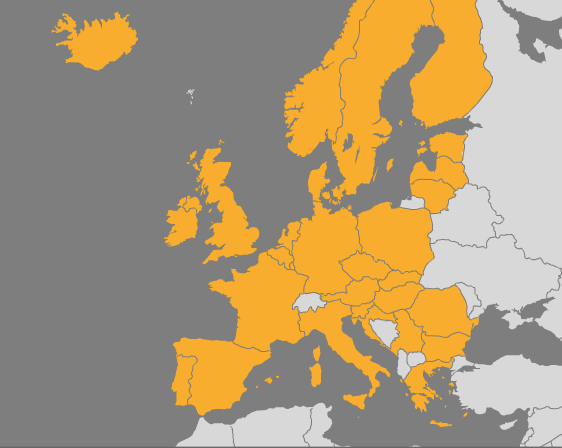
\includegraphics[height=5.0in]{_media/french/french_pix10_europa_map.png}
% %   \caption{Countries represented in META-NET}
% %   \label{fig:metanet_countries}
% % \end{center}
% % \end{figure*}

% META-NET stimulates and promotes multilingual technologies for all European languages. The technologies enable automatic translation, content production, information processing and knowledge management for a wide variety of applications and subject domains. The network wants to improve current approaches, so better communication and cooperation across languages can take place. Europeans have an equal right to information and knowledge regardless of language.

% META-NET launched on 1 February 2010 with the goal of advancing research in language technology (LT). The network supports a Europe that unites as a single digital market and information space. META-NET has conducted several activities that further its goals. META-VISION, META-SHARE and META-RESEARCH are the network's three lines of action.

% % \begin{figure*}[!ht]
% % \begin{center}
% %   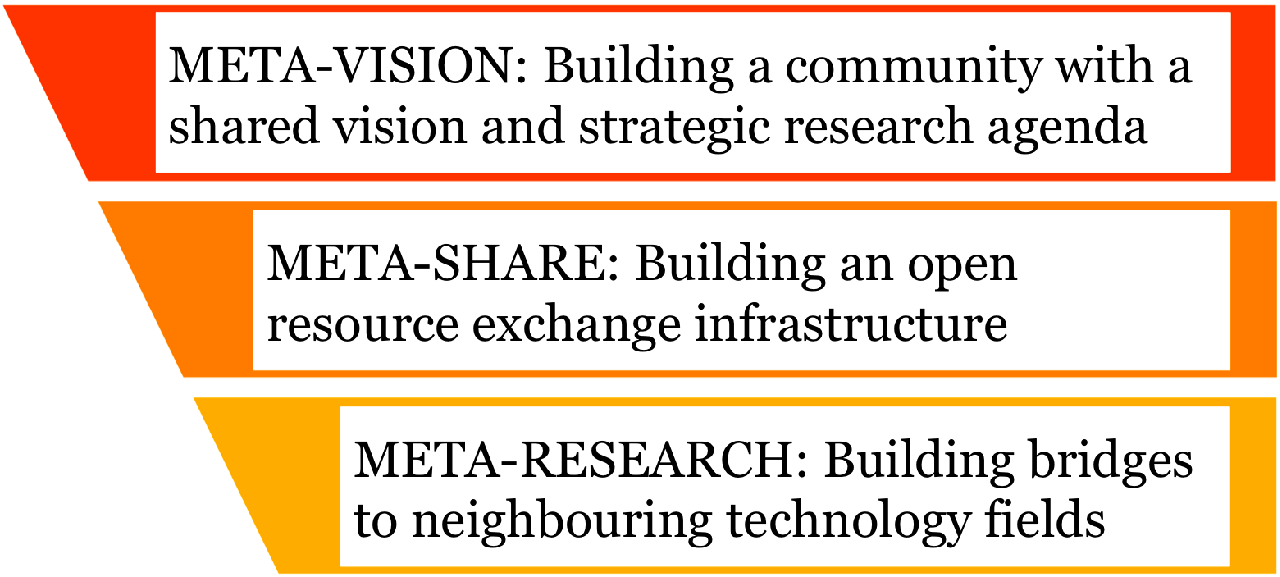
\includegraphics[width=3.0in]{_media/french/meta_3lines}\\
% %   \caption{The three META-NET action lines}
% %   \label{fig:metanetactionlines}
% % \end{center}
% % \end{figure*}

% \textbf{META-VISION} fosters a dynamic and influential stakeholder community that unites around a shared vision and a common strategic research agenda (SRA). The main focus of this activity is to build a coherent and cohesive LT community in Europe by bringing together representatives from highly fragmented and diverse groups of stakeholders. In the first year of META-NET, presentations at the FLaReNet Forum (Spain), Language Technology Days (Luxembourg), JIAMCATT 2010 (Luxembourg), LREC 2010 (Malta), EAMT 2010 (France) and ICT 2010 (Belgium) centred on public outreach. According to initial estimates, META-NET has already contacted more than 2,500 LT professionals to develop its goals and visions with them. At the META-FORUM 2010 event in Brussels, META-NET communicated the initial results of its vision building process to more than 250 participants. In a series of interactive sessions, the participants provided feedback on the visions presented by the network. 

% \textbf{META-SHARE} creates an open, distributed facility for exchanging and sharing resources. The peer-to-peer network of repositories will contain language data, tools and Web services that are documented with high-quality metadata and organised in standardised categories. The resources can be readily accessed and uniformly searched. The available resources include free, open source materials as well as restricted, commercially available, fee-based items. META-SHARE targets existing language data, tools and systems as well as new and emerging products that are required for building and evaluating new technologies, products and services. The reuse, combination, repurposing and re-engineering of language data and tools plays a crucial role. META-SHARE will eventually become a critical part of the LT marketplace for developers, localisation experts, researchers, translators and language professionals from small, mid-sized and large enterprises. META-SHARE addresses the full development cycle of LT - from research to innovative products and services. A key aspect of this activity is establishing META-SHARE as an important and valuable part of a European and global infrastructure for the LT community. 

% \textbf{META-RESEARCH} builds bridges to related technology fields. This activity seeks to leverage advances in other fields and to capitalise on innovative research that can benefit language technology. In particular, this activity wants to bring more semantics into machine translation (MT), optimise the division of labour in hybrid MT, exploit context when computing automatic translations and prepare an empirical base for MT. META-RESEARCH is working with other fields and disciplines, such as machine learning and the Semantic Web community. META-RESEARCH focuses on collecting data, preparing data sets and organising language resources for evaluation purposes; compiling inventories of tools and methods; and organising workshops and training events for members of the community. This activity has already clearly identified aspects of MT where semantics can impact current best practices. In addition, the activity has created recommendations on how to approach the problem of integrating semantic information in MT. META-RESEARCH is also finalising a new language resource for MT, the Annotated Hybrid Sample MT Corpus, which provides data for English-German, English-Spanish and English-Czech language pairs. META-RESEARCH has also developed software that collects multilingual corpora that are hidden on the Web.
% \end{multicols}

\cleardoublepage

\appendix
\addtocontents{toc}{\protect\bigskip}

\phantomsection\bsection[Bibliographie -- Bibliography]{Bibliographie --- Bibliography}

Bureau Van Dijk, Technologies de la Langue en Europe : Marché et Tendances, Ministère de la Recherche, mars 2007\\


European Federation of National Institutions for Language (EFNIL),\\
Language Legislation in Europe.\\
\url{http://www.efnil.org/documents/language-legislation-version-2007}\\


Lewis, M. Paul (ed.), 2009. Ethnologue: Languages of the World, Sixteenth edition. Dallas, Tex.: SIL International. Online version: \url{http://www.ethnologue.com}\\


``Benchmarking HLT progress in Europe'' EUROMAP study, 2003.
\\

Forum des Droits sur l’Internet, «~Internet et Développement Durable~: Langues et Internet~»,\\
Report, 22.12.2009 \url{http://www.foruminternet.org/institution/espace-presse/communiques-de-presse/la-langue-et-internet-le-forum-des-droits-sur-l-internet-publie-une-etude-inedite-2984.html}\\


M. Gasquet-Cyrus, C. Petitjean, «~Le poids des langues~», L’Harmattan, 2009\\

GRRIL (APIL) Livre Blanc ``Le traitement automatique des langues dans les industries de l’information'', January 2005\\

Internet World Stats, \url{http://www.internetworldstats.com} Copyright © 2010, Miniwatts Marketing Group. All rights reserved.\\

Jocelyn Pierre, ``La langue au Cœur du numérique. Les enjeux culturels des technologies de la langue'', Rapport pour la DGLF2, février 2007\\

The Language Technology Center, Study on the size of the Language industry in the European Union, DGT ML Studies 08, August 2009. \url{http://ec.europa.eu/dgs/translation/publications/studies/size\_of\_language\_industry\_en.pdf}\\

Nicholas Ostler, The last lingua franca: English until the return of Babel, 2010\\


\phantomsection\bsection[Références -- References]{Références --- References}
\bibliographystyle{unsrt}
%\bibliography{references}
\bibliography{french_references}
  
\cleardoublepage

\phantomsection\bsection[Membres de META-NET -- META-NET Members]{Membres de META-NET --- META-NET Members}
\label{metanetmembers}

\small
\begin{longtable}{llp{105mm}}
  Allemagne & \textcolor{grey1}{Germany} &  Language Technology Lab, DFKI: Hans Uszkoreit, Georg Rehm\\ \addlinespace
  & & Human Language Technology and Pattern Recognition, RWTH Aachen University: Hermann Ney \\ \addlinespace
  & & Department of Computational Linguistics, Saarland University: Manfred Pinkal\\ \addlinespace 
% Dänemark &  \textcolor{grey1}{Denmark} & Centre for Language Technology, University of Copenhagen: \newline Bolette Sandford Pedersen, Bente Maegaard\\ \addlinespace
  Autriche & \textcolor{grey1}{Austria} & Zentrum für Translationswissenschaft, Universität Wien: Gerhard Budin\\ \addlinespace 

  Belgique & \textcolor{grey1}{Belgium} & Computational Linguistics and Psycholinguistics Research Centre, Univ. of Antwerp: Walter Daelemans\\ \addlinespace
  & & Centre for Proc. Speech and Images, Univ. of Leuven: Dirk van Compernolle \\ \addlinespace

  Bulgarie & \textcolor{grey1}{Bulgaria} & Inst. for Bulgarian Lang., Bulgarian Academy of Sciences: Svetla Koeva \\ \addlinespace

  Chypre & \textcolor{grey1}{Cyprus} & Lang. Centre, School of Humanities: Jack Burston\\ \addlinespace

  Croatie & \textcolor{grey1}{Croatia} & Inst. of Linguistics, Faculty of Humanities and Social Science, Univ. of Zagreb: Marko Tadić \\ \addlinespace

  Danemark &  \textcolor{grey1}{Denmark} & Centre for Language Technology, University of Copenhagen: Bolette Sandford Pedersen, Bente Maegaard\\ \addlinespace

  Espagne & \textcolor{grey1}{Spain} & Barcelona Media: Toni Badia \\ \addlinespace 
  & & Institut Universitari de Lingüistica Aplicada, Univ. Pompeu Fabra: Núria Bel \\ \addlinespace 
  & & Aholab Signal Proc. Lab., Univ. of the Basque Country: Inma Hernaez Rioja \\ \addlinespace 
  & & Center for Lang. and Speech Technologies and Applications, Technical Univ. of Catalonia: Asunción Moreno \\ \addlinespace 
  & & Dept. of Signal Proc. and Communications, Univ. of Vigo: Carmen García Mateo \\ \addlinespace 

  Estonie & \textcolor{grey1}{Estonia} & Inst. of Computer Science, Univ. of Tartu: Tiit Roosmaa\\ \addlinespace

  Finlande & \textcolor{grey1}{Finland} & Computational Cognitive Systems Research Group, Aalto Univ.: Timo Honkela\\ \addlinespace
  & & Dept. of General Linguistics, Univ. of Helsinki: Kimmo Koskenniemi, Krister Linden \\ \addlinespace
 
 France & \textcolor{grey1}{France} & Centre National de la Recherche Scientifique, Laboratoire d'Informatique pour la Mécanique et les Sciences de l'Ingénieur: Joseph Mariani \\ \addlinespace
  & & Evaluations and Lang. Resources Distribution Agency: Khalid Choukri\\ \addlinespace 

  Grande-Bretagne & \textcolor{grey1}{UK} & Inst. for Lang., Cognition and Computation, Center for Speech Technology Research, Univ. of Edinburgh: Steve Renals \\ \addlinespace 
  & & Research Inst. of Informatics and Lang. Proc., Univ. of Wolverhampton: Ruslan Mitkov \\ \addlinespace 
  & & School of Computer Science, Univ. of Manchester: Sophia Ananiandou \\ \addlinespace 

  Grèce & \textcolor{grey1}{Greece} & Inst. for Lang. and Speech Proc., R.C. ``Athena'': Stelios Piperidis\\ \addlinespace

  Hongrie & \textcolor{grey1}{Hungary} & Research Inst. for Linguistics, Hungarian Academy of Sciences: Tamás Váradi\\  \addlinespace
  & & Dept. of Telecommunications and Media Informatics, Budapest Univ. of Technology and Economics: Géza Németh and Gábor Olaszy\\ \addlinespace

  Irlande & \textcolor{grey1}{Ireland} & School of Computing, Dublin City Univ.: Josef van Genabith\\ \addlinespace

  Islande & \textcolor{grey1}{Iceland} & School of Humanities, Univ. of Iceland: Eirikur Rögnvaldsson\\ \addlinespace

  Italie & \textcolor{grey1}{Italy} & Consiglio Nazionale Ricerche, Istituto di Linguistica Computazionale ``Antonio Zampolli'': Nicoletta Calzolari\\ \addlinespace
  & & Human Lang. Technology, Fondazione Bruno Kessler: Bernardo Magnini\\ \addlinespace 

  Lettonie & \textcolor{grey1}{Latvia} & Tilde: Andrejs Vasiljevs\\ \addlinespace 
  & & Inst. of Mathematics and Computer Science, Univ. of Latvia: Inguna Skadina\\ \addlinespace

  Lituanie & \textcolor{grey1}{Lithuania} & Inst. of the Lithuanian Lang.: Jolanta Zabarskaitė\\ \addlinespace

  Luxembourg & \textcolor{grey1}{Luxembourg} & Arax Ltd.: Vartkes Goetcherian\\ \addlinespace

  Malte & \textcolor{grey1}{Malta} & Dept. Intelligent Computer Systems, Univ. of Malta: Mike Rosner\\ \addlinespace

  Norvège & \textcolor{grey1}{Norway} & Dept. of Linguistic, Literary and Aesthetic Studies, Univ. of Bergen: Koenraad De Smedt\\ \addlinespace 
  & & Dept. of Informatics, Lang. Technology Group, Univ. of Oslo: Stephan Oepen \\ \addlinespace

  Pays-Bas & \textcolor{grey1}{Netherlands} & Utrecht Inst. of Linguistics, Utrecht Univ.: Jan Odijk\\ \addlinespace 
  & & Computational Linguistics, Univ. of Groningen: Gertjan van Noord\\ \addlinespace

  Pologne & \textcolor{grey1}{Poland} & Inst. of Computer Science, Polish Academy of Sciences: Adam Przepiórkowski, Maciej Ogrodniczuk \\ \addlinespace
  & & Univ. of Łódź: Barbara Lewandowska-Tomaszczyk, Piotr Pęzik\\ \addlinespace
  & & Dept. of Computer Linguistics and Artificial Intelligence, Adam Mickiewicz Univ.: Zygmunt Vetulani \\ \addlinespace

  Portugal & \textcolor{grey1}{Portugal} & Dept. of Informatics, Univ. of Lisbon: Antonio Branco\\ \addlinespace
  & & Spoken Lang. Systems Lab., Inst. for Systems Engineering and Computers: Isabel Trancoso \\ \addlinespace

  République Tchèque& \textcolor{grey1}{Czech Republic} & Inst. of Formal and Applied Linguistics, Charles Univ. in Prague: Jan Hajic \\ \addlinespace

  Roumanie & \textcolor{grey1}{Romania} & Research Inst. for Artificial Intelligence, Romanian Academy of Sciences: Dan Tufis \\ \addlinespace
  & & Faculty of Computer Science, Univ. Alexandru Ioan Cuza: Dan Cristea \\ \addlinespace

  Serbie & \textcolor{grey1}{Serbia} & Faculty of Mathematics, Belgrade Univ.: Dusko Vitas, Cvetana Krstev, Ivan Obradovic \\ \addlinespace
  & & Pupin Inst.: Sanja Vranes \\ \addlinespace  

  Slovaquie & \textcolor{grey1}{Slovakia} & Ludovit Stur Inst. of Linguistics, Slovak Academy of Sciences: Radovan Garabik \\ \addlinespace 

  Slovénie & \textcolor{grey1}{Slovenia} & Jozef Stefan Inst.: Marko Grobelnik \\ \addlinespace 

  Suède & \textcolor{grey1}{Sweden} & Dept. of Swedish Lang., Univ. of Gothenburg: Lars Borin \\ \addlinespace 

  Suisse & \textcolor{grey1}{Switzerland} & Idiap Research Inst.: Hervé Bourlard 
\end{longtable}
\normalsize

\renewcommand*{\figureformat}{}
\renewcommand*{\captionformat}{}

\begin{figure*}[htbp]
  \colorrule{grey3}{\textwidth}{1.5pt}
  \center
  %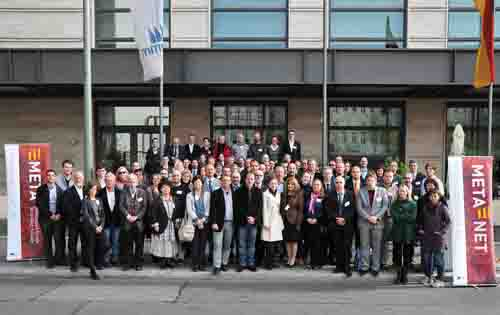
\includegraphics[width=3.0in]{../_media/french/meta-net_team.jpg}
  \fbox{-- META-NET group picture omitted to keep the size of the PDF file small. --}
  \caption{ Une centaine d'experts en technologies de la langue -
    représentant les pays et les langues de META-NET - ont discuté et
    finalisé les résultats-clés et les conclusions de cette
    collection de Livres Blancs lors d'une réunion de META-NET à
    Berlin (Allemagne), les 21 et 22 Octobre 2011. --- \textcolor{grey1}{About
      100 language technology experts -- representatives of the
      countries and languages represented in META-NET -- discussed and
      finalised the key results and messages of the White Paper Series
      at a META-NET meeting in Berlin, Germany, on October 21/22,
      2011.}}
 \medskip
  \colorrule{grey3}{\textwidth}{1.5pt}
\end{figure*}

\cleardoublepage

\bsection[La collection des livres blancs META-NET -- The META-NET White Paper Series]
{Livres Blancs META-NET --- The META-NET\ \ \ \ \ \ White Paper Series}
\label{whitepaperseries}

\vspace*{-5mm}
\centering
  \setlength{\tabcolsep}{2em}
  \begin{tabularx}{\textwidth}{lllll} \toprule\addlinespace
  %\begin{tabulary}{170mm}{LLL} \toprule
  &Allemand & German & Deutsch& \\
  &Anglais & English & English& \\
  &Basque & Basque & euskara& \\
  &Bulgare & Bulgarian & български& \\
  &Catalan & Catalan & català& \\
  &Croate & Croatian & hrvatski& \\
  &Danois & Danish & dansk& \\
  &Espagnol & Spanish & español& \\
  &Estonien & Estonian & eesti& \\
  &Finnois & Finnish & suomi& \\
  &Français & French & français& \\
  &Galicien & Galician & galego& \\
  &Grec & Greek & ελληνικά& \\
  &Hongrois & Hungarian & magyar& \\ %\addlinespace \bottomrule
  &Islandais & Icelandic & íslenska& \\
  &Irlandais & Irish & Gaeilge& \\
  &Italien & Italian & italiano& \\
  &Letton & Latvian & latviešu valoda& \\
  &Lituanien & Lithuanian & lietuvių kalba& \\
  &Maltais & Maltese & Malti& \\
  &Néerlandais & Dutch & Nederlands& \\
  &Norvégien Bokmål & Norwegian Bokmål & bokmål& \\
  &Norvégien Nynorsk & Norwegian Nynorsk & nynorsk& \\
  &Polonais & Polish & polski& \\
  &Portugais & Portuguese & português& \\
  &Roumain & Romanian & română& \\
  &Serbe & Serbian & српски& \\
  &Slovaque & Slovak & slovenčina& \\
  &Slovène & Slovene & slovenščina& \\
  &Suédois & Swedish & svenska& \\
  &Tchèque & Czech & čeština& \\  \addlinespace \bottomrule
\end{tabularx}
